\documentclass[a4paper,12pt,oneside]{book}%extreport
\usepackage{times} 
% \usepackage{multibib}
\usepackage{lipsum}
\usepackage{appendix}
\usepackage[shortlabels]{enumitem}
\usepackage{booktabs}
\usepackage{rotating} % Rotating table
\usepackage{hhline}
\usepackage{colortbl}
\usepackage{afterpage}
\usepackage{mathtools} %Fixes/improves amsmath
\usepackage{setspace}
\usepackage[utf8]{vietnam} 
\usepackage{amstext, amsmath,latexsym,amsbsy,amssymb, amssymb,amsthm,amsfonts,multicol, nccmath}
\usepackage[left=3cm,right=2cm,top=2.5cm,bottom=3cm,footskip=40pt]{geometry}
\usepackage{pdflscape}
\usepackage{apacite}
\usepackage{tikz}
\usepackage{array}
\newcolumntype{C}[1]{>{\centering\let\newline\\\arraybackslash\hspace{0pt}}m{#1}}
\usetikzlibrary{calc}
\usepackage{tabularx}
\usepackage{multicol}
\usepackage{array,color,colortbl}
\setcounter{secnumdepth}{4}
 %\usepackage[square,numbers]{natbib}
\usepackage[square, comma, numbers, sort&compress]{natbib}
\setlength{\parindent}{1cm}
\usepackage{color}
\usepackage{indentfirst}
\usepackage{exscale,eucal}
\usepackage{fancyhdr}
\usepackage{fncychap}
\usepackage[chapter]{algorithm}
\usepackage{multirow}
\usepackage{graphicx}
\usepackage{algpseudocode}
\usepackage{tabularx,multicol,multirow,longtable}
\usepackage{etoolbox}
\usepackage{tikz}	\usetikzlibrary{calc,arrows,decorations.pathmorphing,backgrounds,positioning,fit,shapes,decorations.shapes, shapes.geometric, decorations.pathreplacing, decorations.text}
 
	\tikzstyle{block} = [draw,rectangle,thick,minimum height=2em,minimum width=2em,drop shadow,fill=blue!50]
	\tikzstyle{sum} = [draw,circle,inner sep=0mm,minimum size=2mm]
	\tikzstyle{connector} = [->,thick]
	\tikzstyle{line} = [very thick]
	\tikzstyle{branch} = [circle,inner sep=0pt,minimum size=1mm,fill=black,draw=black]
	\tikzstyle{axes} = [->,>=stealth',semithick]
	\tikzstyle{important line} = [very thick,draw=red]
	\tikzstyle{important text} = [rounded corners,fill=red!10,inner sep=1ex]
\usepackage{circuitikz}
\usepackage{pgfplots}
\pgfplotsset{compat=1.16}
\usepackage[numbers]{natbib}
\usepackage{titlesec}
\usepackage[labelsep=period]{caption}
\usepackage{subfigure}
\DeclareCaptionFormat{myformat}{\fontsize{13}{15}\selectfont#1#2#3}
\captionsetup{format=myformat}
\usepackage{titletoc}
\titlelabel{\thetitle.\,\,}
\titleformat{\chapter}[display] 
  {\fontsize{14}{16}\selectfont\bfseries\centering}
  {\MakeUppercase{\chaptertitlename}\ \thechapter}{0pt}{\fontsize{14}{16}\selectfont\MakeUppercase}
\titlespacing{\chapter}{0pt}{0pt}{40pt} 
\titleformat*{\section}{\fontsize{14}{14}\selectfont\bfseries}
\titleformat*{\subsection}{\fontsize{14}{14}\selectfont\bfseries\slshape}
\titleformat*{\subsubsection}{\fontsize{14}{14}\slshape}
\titleformat*{\paragraph}{\large\bfseries}
\titleformat*{\subparagraph}{\large\bfseries}
\graphicspath {{figures/}}

\titlespacing\section{0pt}{6pt plus 4pt minus 2pt}{1pt plus 2pt minus 2pt} 
\titlespacing\subsection{0pt}{6pt plus 4pt minus 2pt}{1pt plus 2pt minus 2pt}
\titlespacing\subsubsection{0pt}{6pt plus 4pt minus 2pt}{0pt plus 2pt minus 2pt}
\titlespacing\subsubsubsection{0pt}{6pt plus 4pt minus 2pt}{0pt plus 2pt minus 2pt}

\usepackage[subfigure]{tocloft} 

\cftsetpnumwidth{20pt}
\titlecontents{chapter}
  [0pt]
  {}
  {\fontsize{13.5}{14}\selectfont\MakeUppercase{\chaptername}\ \thecontentslabel.\,\,}
  {}
  {\cftdotfill{\cftdotsep}\contentspage} 
	\renewcommand{\cftsecaftersnum}{.}%
	\renewcommand{\cftsubsecaftersnum}{.}%

\usetikzlibrary{calc}
\newtheorem{definition}{\bf Định nghĩa}[chapter]
\newtheorem{theorem}{\bf Định lý}[chapter]
\newtheorem{lemma}{\bf Bổ đề}[chapter]

\renewcommand{\cftfigfont}{Hình~}
\renewcommand{\cfttabfont}{Bảng~ }
\floatname{algorithm}{Thuật toán}
\makeatletter
\renewcommand\@biblabel[1]{[#1]}
\renewcommand\harvardyearleft{\unskip~(}
\renewcommand\harvardyearright{\unskip )}
\makeatother
\renewcommand{\baselinestretch}{1.4}
\flushbottom
\renewcommand*{\bibfont}{\fontsize{13}{16}\selectfont}

\usepackage[hidelinks, unicode]{hyperref}

\begin{document}
\fontsize{13}{15.5}\selectfont

\pagestyle{empty}
\begin{titlepage}
    \centering
\begin{tikzpicture}[overlay,remember picture]
\centering
\draw[line width = 3pt] ($(current page.north west) + (1.215in,-0.7in)$) rectangle ($(current page.south east) + (-0.7in,0.7in)$);
\draw (0,-24.5) node[above]{\fontsize{12}{12}\selectfont{\textbf{HÀ NỘI - 2020}}};
\end{tikzpicture}
\vspace{-1cm}
\begin{center}
\MakeUppercase{\textbf{\fontsize{12}{12}\selectfont{Đại học quốc gia hà nội}}}

\noindent{\textbf {\MakeUppercase{\fontsize{12}{12}\selectfont {trường đại học công nghệ}}}}\\
%}
	\vspace{-0.5cm}
%\noindent\rule{10cm}{0.7pt}
\vspace{2cm}
\begin{figure} [!htb]
	\centering
	
\includegraphics[width=0.2\linewidth]{figures/UET_logo.jpg}
	\label{fig:uetlogo}
\end{figure}
\vspace{1.5cm}

		
	{\textbf {\fontsize{14}{14}\selectfont{ĐỖ HẢI SƠN}}}\\
	\vspace{2cm}
{
{\textbf {\MakeUppercase{\fontsize{17}{17}\selectfont{Xây dựng hệ thống xác định hướng sóng đến}}}}\\[3pt]
{\textbf {\MakeUppercase{\fontsize{17}{17}\selectfont{Sử dụng thuật toán MUSIC trên thiết bị SDR}}}}\\[3pt]
%{\textbf {\MakeUppercase{\fontsize{17}{18}\selectfont{tín hiệu y-sinh được thu thập không đầy đủ}}}}\\
}
\vspace{3cm}
\MakeUppercase{\textbf{\fontsize{14}{14}\selectfont{{Khóa luận tốt nghiệp đại học hệ chính quy}}}}\\[3pt]
{\fontsize{14}{14}\textbf{\selectfont{Ngành: Công nghệ kỹ thuật điện tử, Truyền thông}}}
\end{center}


\end{titlepage}


\newpage
\pagestyle{plain}
\pagenumbering{gobble}
%\addcontentsline{toc}{chapter}{Trang phụ bìa}

\begin{center}
	\begin{tikzpicture}[overlay,remember picture]
\draw[line width = 3pt] ($(current page.north west) + (1.2in,-0.7in)$) rectangle ($(current page.south east) + (-0.7in,0.7in)$);
\draw (0,-24.2) node[above]{\fontsize{12}{12}\selectfont{\textbf{HÀ NỘI - 2020}}};
\end{tikzpicture}
\end{center}
\vspace{-1.5cm}
	\begin{center}
{\MakeUppercase{\textbf{\fontsize{12}{12}\selectfont{Đại học quốc gia hà nội}}}}

\noindent\textbf {\MakeUppercase{\fontsize{12}{12}\selectfont{trường đại học công nghệ}}}\\
	\vspace{-0.5cm}
%\noindent\rule{10cm}{0.7pt}
\vspace{4cm}
		

	{\textbf {\fontsize{14}{14}\selectfont{ĐỖ HẢI SƠN}}}\\
	\vspace{1.5cm}

{\textbf {\MakeUppercase{\fontsize{17}{17}\selectfont{Xây dựng hệ thống xác định hướng sóng đến}}}}\\[3pt]
{\textbf {\MakeUppercase{\fontsize{17}{17}\selectfont{Sử dụng thuật toán MUSIC trên thiết bị SDR}}}}\\[3pt]

\vspace{3cm}
\MakeUppercase{\textbf{\fontsize{14}{14}\selectfont{{Khóa luận tốt nghiệp đại học hệ chính quy}}}}\\[3pt]
{\fontsize{14}{14}\textbf{\selectfont{Ngành: Công nghệ kỹ thuật điện tử, Truyền thông}}}

\end{center}
\vspace{1.5cm}
		\begin{tabularx}
				{\linewidth}{>{\setlength\hsize{.0\hsize}}X>{\setlength\hsize{0.8\hsize}}X}
										& \fontsize{14}{14}\textbf{\selectfont{Cán bộ hướng dẫn: TS. Trần Thị Thúy Quỳnh}}
										%&\MakeUppercase{\fontsize{14}{14}\textbf{\selectfont{TS. Trần Thị Thúy Quỳnh}}}
										%&\MakeUppercase{\fontsize{14}{14}\selectfont{2. GS. TS. Đỗ Ngọc Minh}}
	\end{tabularx}
	





\newpage
\def\baselinestretch{1.3}
\pagestyle{plain}
\pagenumbering{gobble}
\clearpage
\phantomsection

\addcontentsline{toc}{chapter}{Lời cam đoan}
\chapter*{Lời cam đoan}

Tôi xin cam đoan khóa luận tốt nghiệp \textbf{Xây dựng hệ thống xác định hướng sóng đến sử dụng thuật toán MUSIC trên thiết bị SDR} là công trình nghiên cứu thực sự của tôi, được thực hiện dựa trên cơ sở lý thuyết, kiến thức chuyên ngành dưới sự hướng dẫn khoa học của TS. Trần Thị Thúy Quỳnh.

Tôi xin cam đoan những công việc trong khóa luận thực hiện chưa từng được các tác giả khác đề xuất. Với sự hiểu biết của mình, tôi chắc chắn các số liệu, kết quả trong khóa luận là trung thực và chưa được công bố ở đâu và trong bất cứ công trình nào trừ công trình của tác giả và tài liệu tham khảo.

Nếu có gì sai trái, tôi xin hoàn toàn chịu trách nhiệm.

\vspace{1cm}
\hspace{7cm}\textit{Hà Nội, ngày ... tháng ... năm 2020}

\hspace{9.4cm}\textbf{Sinh viên}
\vspace{2.5cm}


\hspace{9.3cm}\textbf{Đỗ Hải Sơn}


\newpage
\clearpage
\phantomsection

\addcontentsline{toc}{chapter}{Lời cảm ơn}
\chapter*{Lời cảm ơn}

\textit{Tôi xin chân thành cảm ơn TS. Trần Thị Thúy Quỳnh, người đã dẫn dắt, định hướng cho tôi trong những nghiên cứu về hệ thống tìm hướng sóng đến. Tôi cũng xin cảm ơn các thầy, cô Khoa Điện tử - Viễn thông và các thầy cô phản biện đã cho nhiều góp ý giúp tôi khắc phục những điểm còn hạn chế trong khóa luận.}

\textit{Tôi cũng xin cảm ơn bạn Trần Đức Mạnh K61ĐB cùng các bạn trong bộ môn Thông tin Vô tuyến đã hỗ trợ tôi rất nhiều trong việc thực nghiệm hệ thống.}

\vspace{1cm}
\hspace{7cm}\textit{Hà Nội, ngày ... tháng ... năm 2020}

\hspace{9.4cm}\textbf{Sinh viên}
\vspace{2.5cm}


\hspace{9.3cm}\textbf{Đỗ Hải Sơn}

 
\newpage
\clearpage
\phantomsection

\addcontentsline{toc}{chapter}{Tóm tắt}
\chapter*{\fontsize{13}{13}\selectfont{Tóm tắt}}
\fontsize{12}{12}\selectfont{
\noindent\textbf{Tóm tắt:}
Hệ tìm phương, hay còn gọi là tìm hướng sóng đến (DOA), luôn đóng vai
trò quan trọng trong các ứng dụng: thông tin, định vị, giám sát, dẫn đường, tìm kiếm cứu nạn,... Với sự phát triển vượt bậc của xử lý tín hiệu, hệ tìm phương sử dụng thuật toán MUSIC cho phép xác định hướng sóng đến của nhiều nguồn phát ở độ chính xác, độ phân giải cao, cấu trúc mảng anten tùy ý, điều mà các hệ tìm phương truyền thống không thể. Các thiết bị vô tuyến định nghĩa bằng phần mềm SDR kết hợp với phần mềm GNU Radio được mong đợi sẽ trở thành công nghệ thống trị truyền thông vô tuyến trong tương lai. Bắt kịp xu thế đó, trong khóa luận này sẽ tập trung tìm hiểu về phần cứng và phần mềm cho SDR: BladeRF x115, lập trình các khối  phục vụ DOA trên GNU Radio. Qua đó triển khai thuật toán tìm phương MUSIC trên hệ BladeRF để kiểm nghiệm khả năng đồng bộ và kết quả ước lượng hướng sóng đến của hệ.

\vspace{0.5cm}
\noindent\textit{\textbf{Từ khóa:}} \textit{DOA, MUSIC, SDR, GNU Radio.}
}
\newpage
\pagenumbering{roman}


\setlength{\parindent}{1cm}
\setlength{\parskip}{0.6ex}

\fontsize{13}{16}\selectfont
\renewcommand{\contentsname}{\vspace{-70pt}\centerline{\fontsize{14}{16}\selectfont\MakeUppercase{Mục lục}}}
\clearpage
\phantomsection
\addcontentsline{toc}{chapter}{Mục lục}
\tableofcontents
\clearpage
\clearpage
\phantomsection

\addcontentsline{toc}{chapter}{Tóm tắt}
\chapter*{\fontsize{13}{13}\selectfont{Tóm tắt}}
\fontsize{12}{12}\selectfont{
\noindent\textbf{Tóm tắt:}
Hệ tìm phương, hay còn gọi là tìm hướng sóng đến (DOA), luôn đóng vai
trò quan trọng trong các ứng dụng: thông tin, định vị, giám sát, dẫn đường, tìm kiếm cứu nạn,... Với sự phát triển vượt bậc của xử lý tín hiệu, hệ tìm phương sử dụng thuật toán MUSIC cho phép xác định hướng sóng đến của nhiều nguồn phát ở độ chính xác, độ phân giải cao, cấu trúc mảng anten tùy ý, điều mà các hệ tìm phương truyền thống không thể. Các thiết bị vô tuyến định nghĩa bằng phần mềm SDR kết hợp với phần mềm GNU Radio được mong đợi sẽ trở thành công nghệ thống trị truyền thông vô tuyến trong tương lai. Bắt kịp xu thế đó, trong khóa luận này sẽ tập trung tìm hiểu về phần cứng và phần mềm cho SDR: BladeRF x115, lập trình các khối  phục vụ DOA trên GNU Radio. Qua đó triển khai thuật toán tìm phương MUSIC trên hệ BladeRF để kiểm nghiệm khả năng đồng bộ và kết quả ước lượng hướng sóng đến của hệ.

\vspace{0.5cm}
\noindent\textit{\textbf{Từ khóa:}} \textit{DOA, MUSIC, SDR, GNU Radio.}
}
\newpage
\clearpage
\phantomsection
\addcontentsline{toc}{chapter}{Danh mục hình vẽ}
\renewcommand{\listfigurename}{\vspace{-70pt}\centerline{\fontsize{14}{16}\selectfont{\MakeUppercase{Danh mục   hình vẽ}}}}
\listoffigures
\fontsize{13}{16}\selectfont
\newpage
\clearpage
\phantomsection
\addcontentsline{toc}{chapter}{Danh mục bảng biểu}
\renewcommand{\listtablename}{\vspace{-70pt}\centerline{\fontsize{14}{16}\selectfont{\MakeUppercase{Danh mục bảng biểu}}}}
\listoftables
\fontsize{13}{16}\selectfont
\newpage

\pagenumbering{arabic}
\pagestyle{plain}

\clearpage
\phantomsection

\addcontentsline{toc}{chapter}{{Mở đầu}}
\chapter*{Mở đầu}
\noindent{\Large \textbf{Lý do chọn đề tài}}

Trong thời đại 4.0 ngày nay, việc xác định hướng đến của đối tượng là nhu cầu không thể thiếu để xây dựng các hệ thống thông minh (xe tự hành, robot tự động, kết hợp với định vị để chỉ đường,…) cũng như những mục đích về an ninh như dò những máy phá sóng dựa trên tần số máy tạo ra, hay định vị hướng tín hiệu cấp cứu tàu thuyền trên biển để ứng cứu kịp thời.

Direction of Arrival (DOA) hay ước lượng hướng sóng đến của tín hiệu tại một điểm đặt mảng anten, hệ thống DOA phải có các đặc tính: độ phân giải cao, ổn định, thích hợp với các thông số đầu vào khác nhau. Thuật toán MUSIC là một phương pháp phổ biến để ước lượng hướng sóng đến với nhiều ưu điểm về độ phân giải so với các thuật toán búp sóng cũng như độ phức tạp thuật toán ở mức trung bình, có thể xác định hướng của nhiều tín hiệu đến với nhiều kiểu điều chế khác nhau và cấu trúc mảng anten tùy ý.

Với ưu điểm truyền/nhận được nhiều loại chuẩn tín hiệu, ở tần số có thể tùy chỉnh dựa trên phần mềm nạp vào, các thiết bị vô tuyến định nghĩa bằng phần mềm SDR kết hợp với phần mềm GNU Radio được mong đợi sẽ trở thành công nghệ thống trị trong truyền thông vô tuyến. Bắt kịp xu thế đó, trong khóa luận này sẽ tập trung nghiên cứu đề tài: \textbf{Xây dựng hệ thống xác định hướng sóng đến sử dụng thuật toán MUSIC trên thiết bị SDR} nhằm thực hiện đồng bộ hệ BladeRF và triển khai xác định hướng sóng đến trên hệ BladeRF để kiểm nghiệm tính chính xác của hệ DOA trong môi truyền thực tế.
\vspace{0.5cm}

\noindent{\Large \textbf{Phương pháp nghiên cứu}}

Trong khóa luận, để đạt được mục đích nghiên cứu, sinh viên đã tìm
hiểu các tài liệu, bài báo, tạp chí quốc tế,... có uy tín, thực hiện việc tính toán mô hình dữ liệu, phân tích số học để đưa ra các hướng giải quyết hợp lý, và sau đó kiểm nghiệm lại kết quả bằng hình thức mô phỏng trên Matlab, GNU Radio cuối cùng là thực nghiệm trên hệ BladeRF thực.

Cụ thể các phương pháp nghiên cứu sau đã được sử dụng trong khóa luận:

\renewcommand{\labelitemi}{$-$}
\begin{itemize}
	\item Sử dụng thuật toán Delay and Sum, Capon và MUSIC xác định hướng sóng đến cho mô hình tính hiệu băng hẹp.
	\item Sử dụng CRB: xác định ngưỡng phân giải của hệ anten ULA.
	\item Vận dụng tương quan chéo ước lượng độ lệch mẫu từ hệ SDR.
	\item Vận dụng thuật toán MUSIC tìm sự sai khác pha giữa các tín hiệu.
\end{itemize} 
\vspace{0.3cm}

\noindent{\Large \textbf{Nội dung nghiên cứu}}

\renewcommand{\labelitemi}{$-$}
\begin{itemize}
	\item Tìm hiểu, mô phỏng và đánh giá độ phân giải của một số thuật toán ước lượng nhiều nguồn tín hiệu phổ biến, có thể áp dụng cho cấu trúc mảng tùy ý, bao gồm: CBF, Capon, MUSIC, ML.
	\item Tìm hiểu tổng quan về thiết bị SDR và phần mềm GNU Radio.
	\item Tìm hiểu về BladeRF x115 và lập trình khối trên GNU Radio.
	\item Đồng bộ hệ BladeRF x115 cho việc triển khai hệ DOA.
	\item Kiểm nghiệm thực tế trên hệ BladeRF thực, đánh giá kết quả ước lượng DOA.
\end{itemize} 
\vspace{0.3cm}

\noindent{\Large \textbf{Đóng góp của đề tài}}

Với sự hiểu biết của sinh viên, những kết quả nghiên cứu trong khóa luận đã đạt được mục đích nghiên cứu đề ra. Những kết quả này bao gồm:

\renewcommand{\labelitemi}{$-$}
\begin{itemize}
	\item Tìm hiểu tổng quan về các hệ thống DOA.
	\item Tổng quan về thiết bị SDR: BladeRF x115 và phần mềm GNU Radio.
	\item Các phương pháp đồng bộ hóa hệ thu SDR.
	\item Ứng dụng thuật toán MUSIC vào thiết bị SDR thời gian thực.
	\item Đánh giá, phân tích kết quả thu được với kết quả mô phỏng.
\end{itemize} 

\noindent{\Large \textbf{Bố cục của khóa luận}}
\vspace{0.5cm}

Nội dung chính của khóa luận được trình bày như sau:

\renewcommand{\labelitemi}{$-$}
\begin{itemize}
	\item Mở đầu: Trình bày mục đích, phương pháp nghiên cứu, nội dung, đóng góp và bố cục của khóa luận.
	\item Chương 1: Tổng quan về các hệ thống xác định hướng sóng đến – Trình bày các công nghệ xác định hướng sóng đến điển hình hiện nay và chi tiết về hệ tìm hướng sóng đến bằng thuật toán MUSIC.
	\item Chương 2: Triển khai thuật toán MUSIC trên thiết bị SDR – Tìm hiểu tổng quan về phần mềm GNU Radio và thiết bị SDR, phương pháp tạo khối trên GNU Radio và giải quyết việc đồng bộ hệ SDR.
	\item Chương 3: Kết quả mô phỏng, thực nghiệm hệ thống – Sử dụng dữ liệu mô phỏng BladeRF trên GNU Radio xác định hướng sóng đến và thực nghiệm hệ thống với tín hiệu BladeRF thực. Qua đó so sánh, nhận xét về kết quả thu được.
	\item Kết luận và hướng nghiên cứu tiếp theo: Đưa ra kết luận về việc sử dụng thiết bị SDR trong việc xác định hướng sóng đến và đề xuất các giải pháp để cải thiện hệ thống.
\end{itemize} 
\newpage
\clearpage
\phantomsection

\setcounter{chapter}{0}
\chapter[{TỔNG QUAN VỀ CÁC HỆ THỐNG XÁC ĐỊNH HƯỚNG SÓNG ĐẾN}]{Tổng quan về các hệ thống xác định hướng sóng đến}

Công nghệ xác định hướng sóng đến không dây có lịch sử phát triển lâu đời, bắt đầu ngay từ khi truyền thông không dây ra đời vào đầu thế kỷ $20^{th}$, và trong suốt chiều dài lịch sử, rất nhiều phương pháp đã được đề xuất. Bắt đầu với những nghiên cứu như sử dụng mạch dao động vòng kín để truyền nhận sóng không dây cũng như xác định hướng đến bằng cách sử dụng mảng anten định hướng (dipoles, loop, ...) của  E. Bellini  và  A. Tosi \cite{Bellini1907} vào năm 1907. Hay cuốn sách Direction and Position Finding by Wireless \cite{Darwin1895} của tác giả Ronald Keen xuất bản lần đầu năm năm 1922 trình bày việc sử dụng mảng pha để giải quyết vấn đề tìm hướng sóng đến. Rất nhiều phương pháp với các cách tiếp cận khác nhau được ra đời sau đó, mục đích chung là nâng cao tính chính xác và độ phân giải của việc xác định hướng sóng đến.

\section{Khái niệm và ứng dụng của hệ xác định hướng sóng đến}

Ước lượng hướng sóng đến của tín hiệu tại một điểm đặt mảng anten phải có các đặc tính: độ phân giải cao, ổn định, thích hợp với các thông số đầu vào khác nhau.

Hiện nay, với sự phát triển của xử lý tín hiệu, các hệ tìm hướng sóng đến xử lý mảng cho phép ước lượng cùng lúc nhiều tham số: hướng sóng đến, thời gian truyền, tần số,... của nhiều tín hiệu mà các hệ tìm phương truyền thống không thể.

Trong vấn đề xử lý tín hiệu thực tế, việc ứng tính được chính xác hướng đến của tất cả các tín hiệu truyền đến mảng anten góp phần tối đa hóa hiệu suất khôi phục lại tín hiệu quan tâm và loại bỏ các tín hiệu khác can thiệp vào.

Một hệ DOA hoàn chỉnh có thể áp dụng cho nhiều mục đích khác nhau: tìm hướng nguồn phát tín hiệu với mục đích phá sóng, tìm hướng tín hiệu cứu cứu hộ, định vị vị trí robot sử dụng trong IoT, xác định vị trí mục tiêu để giám sát hay thăm dò địa chấn, ...
\newpage
\section{Các công nghệ xác định hướng sóng đến điển hình}

\begin{figure} [h]
	\centering
	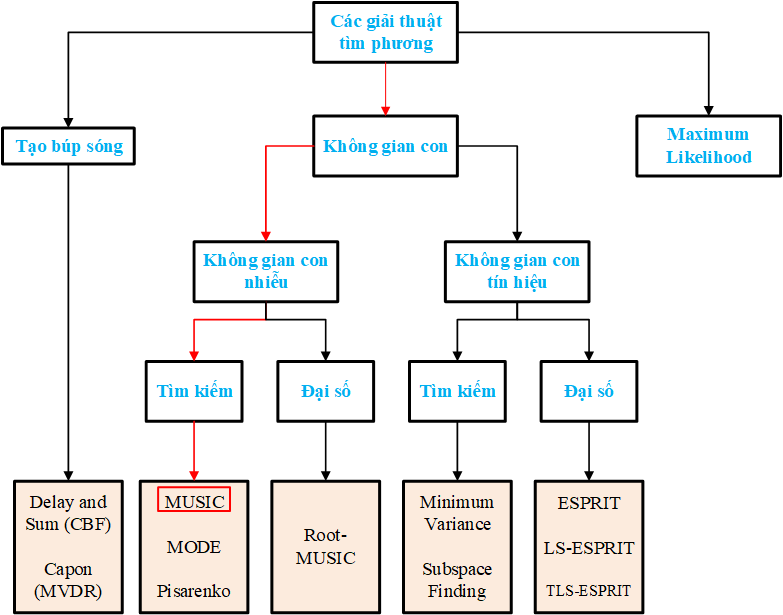
\includegraphics[width= 1\linewidth]{figures/DOA_algorithm.png}
	\caption{Các phương pháp xác định hướng sóng đến}
	\label{fig:overview}
\end{figure}

Trong hình \ref{fig:overview}, các thuật toán tìm hướng sóng đến phổ biến hiện nay được chia vào các nhóm chính, dựa trên hướng tiếp cận để giải quyết bài toán. Mục này sẽ làm nhiệm vụ giới thiệu các thuật toán tìm hướng sóng đến điển hình, mô phỏng chúng trên Matlab, qua đó đưa ra đánh giá về các ưu nhược điểm của từng thuật toán, tập trung chủ yếu vào thuật toán MUSIC sẽ sử dụng trong Chương 3.

Phương pháp thông thường để tính toán hướng sóng đến là dựa trên ý tưởng về tạo búp sóng (beamforming), không khai thác bản chất của vector tín hiệu nhận được $\mathbf{x}(k)$ hoặc mô hình thống kê tín hiệu tạp âm. Các phương pháp thông thường được trình bày dưới đây là phương pháp tạo búp sóng cổ điển (Delay and Sum) và phương pháp phương sai tối thiểu của Capon. Cùng với đó là thuật toán ML là một phương pháp tham số tìm mô hình giống nhất với tín hiệu thu được.

\subsection{Phương pháp tạo búp sóng}

\begin{figure} [!htb]
	\centering
	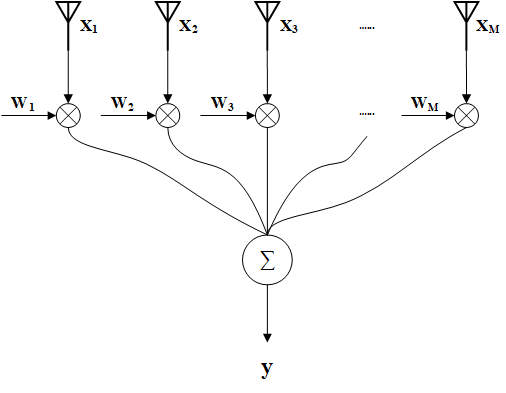
\includegraphics[width=0.7\linewidth]{figures/Beamformer.png}
	\caption{Ví dụ bộ tạo búp sóng tổng quát}
	\label{fig:beamformer}
\end{figure}

Hình \ref{fig:beamformer} biểu diễn sơ đồ bộ tạo búp sóng tổng quát băng hẹp, với tín hiệu đầu ra $\mathrm{y}(t)$ được tính bằng tổng của vector các trọng số $\mathbf{w} = [\mathrm{w}_{1}, ..., \mathrm{w}_{M}]^{T}$ nhân với các dữ liệu thu thập được từ anten.
\begin{equation}
	\mathbf{y}(t) = \mathbf{w}^{H}\mathbf{x}(t)
\end{equation}

Công suất lối ra được tính bởi:
\begin{equation}
	\mathbf{P}_{CBF}(\mathbf{w}) = E[|\mathbf{y}(t)|^{2}] = E[|\mathbf{w}^{H}\mathbf{x}(t)|^{2}] = {\mathbf{w}^{H}}E[\mathbf{x}(t)\mathbf{x}^{H}(t)]\mathbf{w} = \mathbf{w}^{H}\mathbf{R}_{\mathbf{x}}\mathbf{w}
\label{eq:Pcbf}
\end{equation}
với $\mathbf{R}_{\mathbf{x}}$ là ma trận tự tương quan lối vào. Với K mẫu $[\mathrm{y}_{1}, ..., \mathrm{y}_{K}]$, phương trình (\ref{eq:Pcbf}) trở thành:
\begin{equation}
\begin{split}
	\mathbf{P}_{CBF}(\mathbf{w}) &= \frac{1}{K}\sum_{k = 1}^{K}|\mathbf{y}(t)|^{2} = \frac{1}{K}\sum_{k = 1}^{K}\mathbf{w}^{H}\mathbf{x}(k)\mathbf{x}^{H}(k)\mathbf{w} = \mathbf{w}^{H}\tilde{\mathbf{R}}_{\mathbf{x}}\mathbf{w} \\
	\tilde{\mathbf{R}}_\mathbf{x} &= \frac{1}{K} \sum_{k = 1}^{K} \mathbf{x}(k)\mathbf{x}^{H}(k) : \text{ ước lượng của $\mathbf{R}_\mathbf{x}$}
\end{split}
\label{eq:Pcbf1}
\end{equation}

Phổ không gian của thuật toán là công suất lối ra ứng với góc quét. Các góc ứng với đỉnh trong phổ không gian chính là góc sóng đến cần ước lượng. Tới đây, việc chọn vector trọng số cho bộ tạo búp sóng được thực hiện theo nhiều phương pháp, mà dưới đây là hai phương pháp điển hình và thường xuyên được sử dụng nhất là Delay and Sum (hay bộ tạo búp sóng truyền thống) và Capon (hay bộ tạo búp sóng MVDR). 
%Chi tiết thuật toán được trình bày bên dưới:

\begin{itemize}
	\item[$\ast$] \textbf{Delay and Sum (Conventional Beamforming Method)}
\end{itemize}

Phương pháp tạo búp sóng truyền thống hay Delay-and-Sum \cite{Liberti1999} là phương pháp đơn giản nhất trong các kỹ thuật tìm hướng sóng đến bằng việc tạo búp sóng. Ý tưởng của phương pháp là quét qua các vùng góc quan tâm (thường là trong các phần rời rạc) và hướng nào tạo ra công suất đầu ra lớn nhất là được coi là hướng tín hiệu mong muốn cần ước lượng.

Xét một tín hiệu $\mathbf{x}(k)$ có hướng đến so với mảng anten thu là ${\phi}_{0}$, theo mô hình băng hẹp hình \ref{fig:beamformer} với $\mathbf{x}(t) = \sum_{k=1}^{K}\mathbf{a}_{k}(t)\mathbf{s}_{k}(t) + \mathbf{n}(t)$ (được diễn giải chi tiết ở công thức (\ref{eq:rec})), công suất đầu ra của bộ tạo búp sóng được tính bởi:
\begin{equation}
\begin{split}
	\mathbf{P}_{CBF}(\phi_{0}) &= E[|\mathbf{w}^{H}\mathbf{x}(k)|^{2}] = E[|\mathbf{w}^{H}(\mathbf{a}(\phi_{0})\mathbf{s}(k) + \mathbf{n}(k))|^{2}] \\
	&= [|\mathbf{w}^{H}\mathbf{a}(\phi_{0})|^{2}({\mathbf{\sigma}_{\mathbf{s}}}^{2} + {\mathbf{\sigma}_{\mathbf{n}}}^{2})]
\end{split}
\label{eq:barl}
\end{equation}
với $\mathbf{a}(\phi_{0})$ là vector đáp ứng mảng với sóng đến góc $\phi_{0}$, $\mathbf{n}(k)$ là vector tạp âm ở mảng đầu vào, $\sigma_{\mathbf{s}} = E[\mathbf{s}(k)^{2}]$ và $\sigma_{\mathbf{n}} = E[\mathbf{n}(k)^{2}]$ lần lượt là công suất của tín hiệu và tạp âm. Theo công thức (\ref{eq:barl}), công suất đầu ra tối đa khi $\mathbf{w} = \mathbf{a}(\phi_{0})$, hay trong tất cả các vector trọng số có thể, anten thu có mức tăng cao nhất theo hướng $\phi_{0}$ khi $\mathbf{w} = \mathbf{a}(\phi_{0})$. Điều này có được do $\mathbf{w} = \mathbf{a}(\phi_{0})$ căn chỉnh góc của các thành phần tín hiệu đến từ góc $\phi_{0}$ tại mảng anten thu, vậy nên chúng đẩy giá trị công suất lên.

Thay $\mathbf{w} = \mathbf{a}(\phi_{0})$ vào công thức của công suất lối ra ứng với góc quét (\ref{eq:Pcbf1}), phổ không gian vẽ bởi công suất lối ra từ bộ tạo búp sóng truyền thống tương ứng:
\begin{equation}
	\mathbf{P}_{CBF}(\phi) =\mathbf{w}^{H}\tilde{\mathbf{R}}_{\mathbf{x}}\mathbf{w} = \mathbf{a}^{H}(\phi)\tilde{\mathbf{R}}_{\mathbf{x}}\mathbf{a}(\phi)
\end{equation}

Vì là phương pháp đơn giản nhất nên phương pháp tạo búp sóng truyền thống có nhiều nhược điểm: độ rộng của búp sóng lớn dẫn đến khi có nhiều nguồn đến với góc gần nhau, công suất của chúng sẽ bị cộng lại thành một búp sóng duy nhất. Mặc dù có thể tăng độ phân giải bằng cách tăng số lượng máy thu nhưng cách tốt hơn là sử dụng một thuật toán tạo búp sóng khác, đó là Capon được trình bày dưới đây.

\begin{itemize}
	\item[$\ast$] \textbf{Thuật toán tạo búp sóng của Capon}
\end{itemize}

Bộ tạo búp sóng Capon \cite{Capon2009} hay Minimum Variance Distortionless Response cũng là một phương pháp phổ biến để khắc phục hạn chế về độ phân giải của phương pháp CBF. Phương pháp này thực hiện tối thiểu hóa công suất tạp âm và công suất theo các hướng khác, ngoại trừ hướng của tín hiệu đến $\phi_{0}$ vì vậy vector trọng số $\mathbf{w}$ trong phương trình (\ref{eq:capon}) còn được gọi là vector trọng số của búp sóng đáp ứng không méo phương sai tối thiểu (MVDR). Phương pháp này có phương trình tối ưu:
\begin{equation}
	\underset{\mathbf{w}}{\mathbf{min}}\; E[|\mathbf{y}(k)|^{2}] = \underset{\mathbf{w}}{\mathbf{min}}\; \mathbf{w}^{H}\mathbf{R}_{\mathbf{x}}\mathbf{w} \;\;\textrm{với}\;\; \mathbf{w}^{H}\mathbf{a}(\phi_{0}) = 1
\label{eq:capon} 
\end{equation}

Sử dụng phương pháp nhân tử Lagrange,  giải được nghiệm của phương trình (\ref{eq:capon}) là vector trọng số:
\begin{equation}
	\mathbf{w} = \frac{{\mathbf{R}_{\mathbf{x}}}^{-1}\mathbf{a}(\phi)}{\mathbf{a}^{H}(\phi){\mathbf{R}_{\mathbf{x}}}^{-1}\mathbf{a}(\phi)}
\end{equation}

Với nghiệm trên, thay vào (\ref{eq:Pcbf1}), phổ không gian vẽ bởi công suất lối ra từ bộ tạo búp sóng Capon, với các đỉnh của phổ không gian chính là ước lượng hướng sóng đến của tín hiệu tương ứng:
\begin{equation}
	\mathbf{P}_{Capon}(\phi) = \frac{1}{\mathbf{a}^{H}(\phi)\mathbf{R}_{\mathbf{x}}\mathbf{a}(\phi)}
\end{equation}

Hình \ref{fig:CBFvsCapon} là kết quả mô phỏng 2 thuật toán tìm hướng sóng đến CBF và Capon trên Matlab với 2 nguồn phát ở góc 80$^{\circ}$ và 85$^{\circ}$, mảng anten thu gồm 4 phần tử anten đặt thẳng cách đều nhau  $0,5\lambda = 0,5 \times 0,325 (m)$. Có thể thấy phương pháp CBF chỉ nhận diện được một búp sóng ở khoảng góc từ 60$^{\circ}$ đến 100$^{\circ}$ còn Capon đã khắc phục được độ phân giải kém này khi xác định được 2 đỉnh ở 80$^{\circ}$ và 85$^{\circ}$. Tuy nhiên, dễ nhận thấy khi góc đến thu hẹp hơn nữa chỉ 1$^{\circ}$ hay 2$^{\circ}$ thì phương pháp Capon cũng khó có thể phân biệt được. Hơn nữa, phương pháp Capon cần có điều kiện là không có các tín hiệu khác tương quan với tín hiệu cần xác định hướng sóng đến và trong thuật toán có phương trình yêu cầu nghịch đảo ma trận, nếu tăng số phần tử thu lớn có thể dẫn đến tốn kém bộ nhớ.
\begin{figure} [!htb]
	\centering
	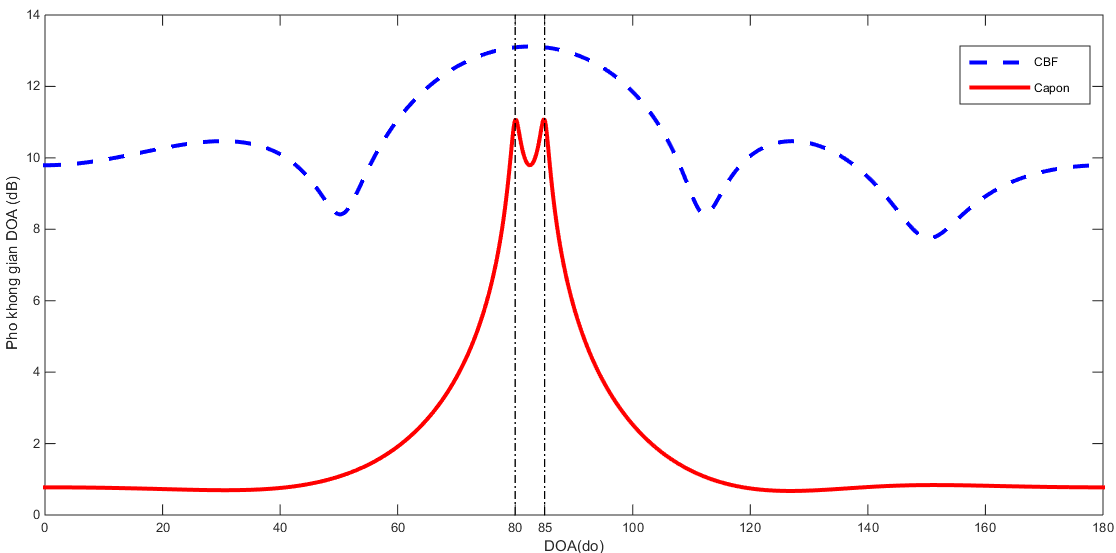
\includegraphics[width=1\linewidth]{figures/CBFvsCapon.png}
	\caption{Mô phỏng thuật toán Delay and Sum và Capon}
	\label{fig:CBFvsCapon}
\end{figure}

\subsection{Thuật toán Maximum Likelihood}

Maximum Likelihood (ML) là một trong những thuật toán đầu tiên được phát triển để tính toán DOA. Tuy không phổ biến bằng thuật toán MUSIC trình bày trong mục 1.3 bên dưới, tuy nhiên do sử dụng phương pháp tham số nên tránh được các vấn đề nhiễu đa đường, tín hiệu tương quan cao, số lượng mẫu nhỏ của các phương pháp dùng phổ \cite{Ziskind1988}.

Với nguyên tắc cơ bản là tìm mô hình dữ liệu giống nhất với dữ liệu được thu thập tại mảng anten thu. Vẫn tiếp tục sử dụng mô hình tín hiệu nguồn như phương trình (\ref{eq:rec}), hàm mật độ xác suất chung của K mẫu thu thập $\mathbf{x}(1), ..., \mathbf{x}(K)$  là:
\begin{equation}
	\mathit{f}(\mathbf{x}) = \prod_{k=1}^{K}\frac{1}{\pi\mathbf{det}[\sigma^2\mathbf{I}]} \cdot  \mathrm{exp}(-\frac{1}{\sigma^2}|\mathbf{x}(k) - A(\Phi)\mathbf{s}(k)|^2)
\end{equation}
với $\mathbf{det}$ là định thức của ma trận. Tiếp theo, loại bỏ các thành phần không phụ thuộc vào $\Phi$, ta có hàm  log likelihood:
\begin{equation}
	L(\Phi) = -Mp\log\sigma^2 - \frac{1}{\sigma^2}\sum_{k=1}^{K}|\mathbf{x}(k) - A(\Phi)\mathbf{s}(k)^2|
\end{equation}

Phương pháp ML thực hiện tìm giá trị cực đại của hàm log likelihood khi thay đổi các giá trị $\Phi$ và $\mathbf{s}$, bỏ qua các giá trị không thay đổi, ta thu được:
\begin{equation}
	\underset{\Phi, \mathbf{s}}{\max} \left[-Mp\log(\frac{1}{Mp}\sum_{k=1}^{K}|\mathbf{x}(k) - A(\Phi)\mathbf{s}(k)|^2)\right]
\label{eq:ML}
\end{equation}

Do $\mathbf{log}$ là một hàm đơn điệu nên tìm cực đại của phương trình (\ref{eq:ML}) tương đương với:
\begin{equation}
	\underset{\Phi, \mathbf{s}}{\min} \left[\sum_{k=1}^{K}|\mathbf{x}(k) - A(\Phi)\mathbf{s}(k)|^2\right]
\label{eq:ML1}
\end{equation}

Các bước tiếp thuộc vấn đề tối ưu hóa phi tuyến tính nhiều chiều và phức tạp, cụ thể được trình bày ở \cite{Ziskind1988}.

\section{Hệ thống xác định hướng sóng đến với thuật toán MUSIC}

Phương pháp phương sai tối thiểu của Capon thường chính xác và được sử dụng rộng rãi, tuy nhiên phương pháp này có một số hạn chế cơ bản trong độ phân giải. Còn phương pháp tham số: ML lại có độ phức tạp cao khi thực hiện tìm kiếm D-D (D chiều). Schmidt đã đưa ra một giải pháp hoàn chỉnh dựa trên thống kê bậc hai cho vấn đề ước lượng DOA, có khả năng áp dụng cho mọi loại tín hiệu với cấu trúc anten tùy ý. Kỹ thuật được đề xuất bởi Schmidt vào năm 1979 với tên gọi: thuật toán phân loại đa tín hiệu (MUSIC) \cite{Schmidt2009a}. Sơ đồ khối của hệ tìm hướng sóng đến sử dụng thuật toán MUSIC được đưa ra trên hình \ref{fig:musicstruct}.

\begin{figure} [!h]
	\centering
	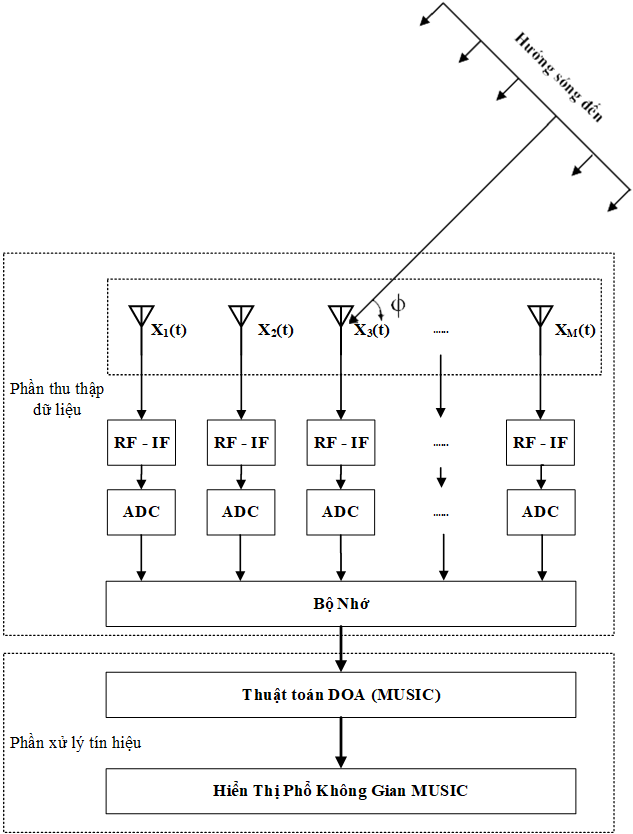
\includegraphics[width=0.75\linewidth]{figures/MuSIC_Structor.png}
	\caption{Sơ đồ khối hệ tìm hướng sóng đến sử dụng thuật toán MUSIC}
	\label{fig:musicstruct}
\end{figure}

Xét D nguồn tín hiệu đến với các hướng không biết trước $\phi_{1}$, ..., $\phi_{D}$ đến mảng anten thu gồm M (điều kiện M > D) phần tử vô hướng được đặt tùy ý trong mặt phẳng ở các tọa độ ($\bar{\mathrm{x}}_1$, $\bar{\mathrm{y}}_1$), ..., ($\bar{\mathrm{x}}_M$, $\bar{\mathrm{y}}_M$).

Vector tín hiệu bên thu nhận được $\mathbf{x}(t) \in \mathbb{C}^{M}$  tại thời điểm \textit{t} được biểu diễn bởi công thức (\ref{eq:rec}), với $\Phi$ = $[\phi_{1}, ..., \phi_{D}]^{T}$ tương ứng với hướng của các nguồn tín hiệu đến mảng anten thu, $\mathbf{A}(\Phi) = [\mathbf{a}(\phi_{1}), ..., \mathbf{a}(\phi_{D})] \in \mathbb{C}^{M  \times D}$ là mà trận chứa các vector đáp ứng mảng $\mathbf{a}(\phi) \in \mathbb{C}^{M}$; $\mathbf{s}(t) \in \mathbb{C}^{D}$ là vector nguồn tín hiệu và $\mathbf{n}(t) \in \mathbb{C}^{M}$ tương ứng là vector tạp âm:
\begin{equation}
\begin{matrix}
\begin{bmatrix}
\mathrm{x}_{1}(t) \\
... \\
\mathrm{x}_{M}(t)
\end{bmatrix}
=
\begin{bmatrix}
 &  & \\ 
\mathbf{a}(\phi_{1}) &...  &\mathbf{a}(\phi_{D})\\ 
 &  & 
\end{bmatrix}
\begin{bmatrix}
\mathrm{s}_{1}(t)\\ 
...\\ 
\mathrm{s}_{D}(t)
\end{bmatrix}
+
\begin{bmatrix}
\mathrm{n}_{1}(t)\\ 
...\\ 
\mathrm{n}_{M}(t)
\end{bmatrix}\\  
\\ \textrm{hay được viết dưới dạng ma trận}\\ \\
\mathbf{x}(t) = \mathbf{A}(\Phi)\mathbf{s}(t) + \mathbf{n}(t)\\ 
\end{matrix}
\label{eq:rec}
\end{equation}

Trong đó, vector đáp ứng mảng được biểu diễn chi tiết như công thức (\ref{eq:resp}) với $\lambda$ là bước sóng của tín hiệu:
\begin{equation}
\mathbf{a}(\phi) = 
\begin{bmatrix}
e^{-j\frac{2\pi}{\lambda}(\bar{\mathrm{x}}_{1}\cos\phi \,+\, \bar{\mathrm{y}}_{1}\sin\phi)}\\ 
...\\ 
e^{-j\frac{2\pi}{\lambda}(\bar{\mathrm{x}}_{M}\cos\phi \,+\, \bar{\mathrm{y}}_{M}\sin\phi)}
\end{bmatrix}
\label{eq:resp}
\end{equation}

Các vector đáp ứng mảng này là các giá trị cần được giả thiết là biết trước tùy theo cấu hình anten, được lưu trữ làm các giá trị chuẩn hóa cần thiết cho mọi bước tính toán; vector tín hiệu và tạp âm (nhiễu trắng) có trung bình bằng 0; vector tạp âm trắng hóa không gian (tạp âm đến mỗi phần tử anten đều có phương sai giống nhau là ${\sigma_{\mathrm{n}}}^{2}$ không tương quan với nhau) và độc lập thống kê với các tín hiệu nguồn.

Ma trận hiệp phương sai trong không gian được biểu diễn bởi công thức (\ref{eq:Ruu}), với $\mathcal{E}$ là ký hiệu của kỳ vọng thống kê, $\mathcal{E}\{\mathbf{s}(t)\mathbf{s}^{H}(t)\} = \mathbf{R}_{\textbf{s}}$, $\mathcal{E}\{\mathbf{n}(t)\mathbf{n}^{H}(t)\} = \mathbf{{{\sigma}_{\mathrm{n}}}^{2}I_{\mathbf{n}}}$ lần lượt là ma trận tương quan của tín hiệu nguồn và của tạp âm, $\mathbf{{I_{n}}} \in \mathbb{C}^{M \times M}$ là ma trận đơn vị. 
\begin{equation}
\begin{split}
	\mathbf{C}_{\mathbf{x}} = \mathbf{R}_{\mathbf{x}} &= 	\mathcal{E}\{\mathbf{x}(t)\mathbf{x}^{H}(t)\}	\\
	&= \mathbf{A}\mathcal{E}\{\mathbf{s}(t)\mathbf{s}^{H}(t)\}\mathbf{A}^{H} + \mathcal{E}\{\mathbf{n}(t)\mathbf{n}^{H}(t)\}	\\
	&= \mathbf{A}\mathbf{R}_{\mathbf{s}}\mathbf{A}^{H} + {\sigma_{\mathbf{n}}}^{2}\mathbf{I}_{\mathbf{n}}
\end{split}
\label{eq:Ruu}
\end{equation}

Tiếp tục khai triển ma trận $\mathbf{R}_{\mathbf{x}}$ thành các giá trị riêng và các vector riêng tương ứng là $\lambda_{m}$ và $\mathbf{e}_{m} (m =1, ..., M)$.
\begin{equation}
\begin{split}
	\mathbf{R}_{\mathbf{x}} &= \sum_{m = 1}^{M} \lambda_{m}\mathbf{e}_{m}{\mathbf{e}_{m}}^{H} = \mathbf{E}\Lambda\mathbf{E}^{H} = \mathbf{E}_{\mathbf{s}}\Lambda_{\mathbf{s}}{\mathbf{E}_{\mathbf{s}}}^{H} + \mathbf{E}_{\mathbf{n}}\Lambda_{\mathbf{n}}{\mathbf{E}_{\mathbf{n}}}^{H} \\
	  &=\mathbf{E}_{\mathbf{s}}\Lambda_{\mathbf{s}}{\mathbf{E}_{\mathbf{s}}}^{H} +  {\mathbf{\sigma}_{\mathbf{n}}}^{2}\mathbf{E}_{\mathbf{n}}{\mathbf{E}_{\mathbf{n}}}^{H} = \mathbf{E}_{\mathbf{s}}\tilde{\Lambda}_{\mathbf{s}}{\mathbf{E}_{\mathbf{s}}}^{H} + {\mathbf{\sigma}_{\mathbf{n}}}^{2}\mathbf{I}_{\mathbf{n}}
\end{split}
\end{equation}
{\renewcommand\labelitemi{}
\begin{itemize}
  \item với $\mathbf{E} = [\mathbf{e}_{1}, ..., \mathbf{e}_{M}]$
  \item \hspace{0.7cm}$\mathbf{E}_{\mathbf{s}} = [\mathbf{e}_{1}, ..., \mathbf{e}_{D}]$
  \item \hspace{0.7cm}$\mathbf{E}_{\mathbf{n}} = [\mathbf{e}_{D+1}, ..., \mathbf{e}_{M}]$ 
  \item \hspace{0.7cm}$\Lambda = diag\{\lambda_{1}, ..., \lambda_{M}\}$
  \item \hspace{0.7cm}$\Lambda_{\mathbf{s}} = diag\{\lambda_{1}, ..., \lambda_{D}\}$
  \item \hspace{0.7cm}$\Lambda_{\mathbf{n}} = diag\{\lambda_{D}, ..., \lambda_{M}\}$
  \item \hspace{0.7cm}$\tilde{\Lambda}_{\mathbf{s}} = \Lambda_{\mathbf{s}} - {\mathbf{\sigma}_{\mathbf{n}}}^{2}\mathbf{I}_{\mathrm{n}}$
\end{itemize}
}
 
Vector riêng $\mathbf{E} = [\mathbf{E}_{\mathbf{s}}, \mathbf{E}_{\mathbf{n}}]$ có thể giả sử để tạo thành một cơ sở trực giao ($\mathbf{E}\mathbf{E}^{H} = \mathbf{E}^{H}\mathbf{E} = \mathbf{I})$. Từ $\mathbf{E}$ có thể tách được ra hai ma trận: ma trận chứa D vector riêng tương ứng với không gian con tín hiệu là $\mathbf{E}_{\mathbf{s}} \triangleq [\mathbf{e}_{1}, ..., \mathbf{e}_{D}]$; ma trận chứa M - D vector riêng tương ứng với không gian con của tạp âm là $\mathbf{E}_{\mathbf{n}} \triangleq [\mathbf{e}_{D+1}, ..., \mathbf{e}_{M}]$. Để phân tích chi tiết các thuộc tính cấu trúc riêng của ma trận hiệp phương sai $\mathbf{R}_{\mathbf{x}}$ tham khảo tại \cite{Schmidt2009a}.


Khi các không gian con đã được xác định, có thể ước tính hướng đến của các tín hiệu mong muốn bằng cách tính phổ không gian MUSIC trên vùng quan tâm:
\begin{equation}
	\mathbf{P}_{MUSIC}(\phi) = \frac{\mathbf{a}^{H}(\phi)\mathbf{a}(\phi)}{\mathbf{a}^{H}(\phi)\mathbf{E}_{\mathbf{n}}{\mathbf{E}_{\mathbf{n}}}^{H}\mathbf{a}({\phi})}
\end{equation}

Thực hiện mô phỏng với thông số mảng thu tương tự như thuật toán Capon trên Matlab, tuy nhiên thay đổi góc của 2 nguồn tín hiệu phát là 80$^{\circ}$ và 82$^{\circ}$, hình \ref{fig:MUSICvsCapon} dưới đây biểu diễn kết quả thu được. Có thể thấy rõ sự vượt trội của thuật toán MUSIC trong việc ước tính DOA.
\begin{figure} [!htb]
	\centering
	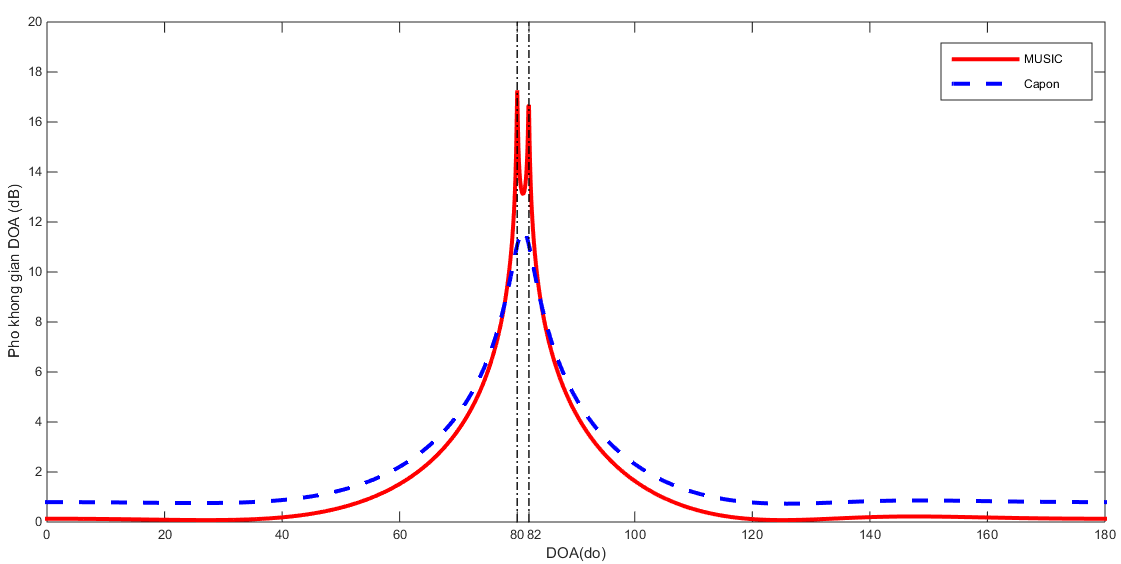
\includegraphics[width=1\linewidth]{figures/MUSICvsCapon.png}
	\caption{Mô phỏng thuật toán MUSIC và Capon}
	\label{fig:MUSICvsCapon}
\end{figure}

\newpage
\clearpage
\phantomsection

\setcounter{chapter}{1}
\chapter[{TRIỂN KHAI THUẬT TOÁN MUSIC TRÊN THIẾT BỊ SDR}]{Triển khai thuật toán MUSIC trên thiết bị SDR}

%\section{Phần mềm GNU Radio}

Chương này sẽ giới thiệu khái quát về lịch sử, cách thức hoạt động của phần mềm GNU Radio và thiết bị vô tuyến định nghĩa bằng phần mềm SDR. Tập trung tìm hiểu về phần cứng của BladeRF và phần mềm trên GNU Radio để thực thi trên BladeRF, cùng với đó là việc đồng bộ hệ nhiều BladeRF trước khi triển khai thuật toán MUSIC trên BladeRF.

\section{Phần mềm GNU Radio và thiết bị vô tuyến định nghĩa bằng phần mềm SDR}

\subsection{Phần mềm GNU Radio}

GNU Radio là bộ công cụ phát triển phần mềm, mã nguồn mở và hoàn toàn miễn phí, cung cấp các khối xử lý tín hiệu để mô phỏng và thực hiện các hệ truyền thông. Phần mềm tương thích với các thiết bị ngoại vi vô tuyến để tạo thành thiết bị vô tuyến được định nghĩa bằng phần mềm (Software Define Radio). GNU Radio sử dụng rộng rãi trong giảng dạy, nghiên cứu cũng như thương mại, hỗ trợ cho việc nghiên cứu các hệ truyền thông không dây và các hệ truyền thông vô tuyến trong thực tế.

Được khởi xướng bởi nhà hảo tâm John Gilmore và trưởng dự án Eric Blossom từ năm 2001 liên tục được phát triển, cho đến năm 2009, Josh Blum phát hành phiên bản GNU Radio Companion 3.2 đầu tiên. Năm 2011, đội ngũ các nhà phát triển lõi của GNU Radio bắt đầu tổ chức hội nghị hàng năm đầu tiên với tên gọi GRCon. Hiện tại, GNU Radio đã phát hành đến phiên bản 3.8 với nhiều cải tiến và liên tục được cập nhật bởi nhà phát hành cùng với các nhà phát triển độc lập \cite{PyBombs}. GNU Radio có sẵn rất nhiều khối được hoàn thiện và sẵn sàng sử dụng, dưới đây là những khối điển hình thường xuyên sử dụng trong hệ truyền thông không dây 2G, 3G, 4G và 5G:
\renewcommand{\labelitemi}{$-$}
\begin{itemize}
\item Waveform Generators 
	\begin{itemize}
		\item[$\diamond$] Signal Source (e.g. Sine, Square, Saw Tooth,...)
		\item[$\diamond$] Noise Source
		\item[$\diamond$] Constant Source
	\end{itemize}
\item Modulator
	\begin{itemize}
		\item[$\diamond$] AM Demod
		\item[$\diamond$] Continuous Phase Modulation
		\item[$\diamond$] PSK Mod / Demod
		\item[$\diamond$] GFSK Mod / Demod
		\item[$\diamond$] QAM Mod / Demod
		\item[$\diamond$] WBFM / NBFM Receive
		\item[$\diamond$] DVB-T / DVB-T2
		\item[$\diamond$] CDMA \cite{Kavitha2015}
		\item[$\diamond$] OFDM \cite{Bloessl2013}
	\end{itemize}
\item  Channel Models 
	\begin{itemize}
		\item[$\diamond$] Channel Model
		\item[$\diamond$] Fading Model
		\item[$\diamond$] Frequency Selective Fading Model
	\end{itemize}
\item Filters
	\begin{itemize}
		\item[$\diamond$] Low / High Pass Filter
		\item[$\diamond$] Band Pass / Reject Filter
		\item[$\diamond$] IIR Filter
		\item[$\diamond$] Decimating FIR Filter
		\item[$\diamond$] Hilbert
		\item[$\diamond$] Root Raised Cosine Filter
		\item[$\diamond$] FFT Filter
	\end{itemize}
\item Fourier Analysis 
	\begin{itemize}
		\item[$\diamond$] FFT
		\item[$\diamond$] FLL Band-Edge
		\item[$\diamond$] Rational Resampler (Synchronizers)
		\item[$\diamond$] PN Correlator
	\end{itemize}
\end{itemize}

Giao diện cho người dùng thông thường là GNU Radio Companion (GRC) được hiển thị như hình \ref{fig:GNURadio}. Với giao diện khá tương đồng với Matlab Simulink, gồm các khối nguồn, xử lý tín hiệu, hiển thị, widget,… dễ dàng chọn lựa, tùy chỉnh và kết nối với nhau thành flow-graph. Tất cả được GRC biên dịch ra file python và đẩy cho GNU Radio xử lý và hiển thị kết quả dựa trên QT GUI (QT Toolkit), hoặc Wx GUI (WxPython, tuy nhiên Wx Python đã bị xóa bỏ ở phiên bản GNU 3.8 do tốc độ đáp ứng chậm).

\begin{figure} [!h]
	\centering
	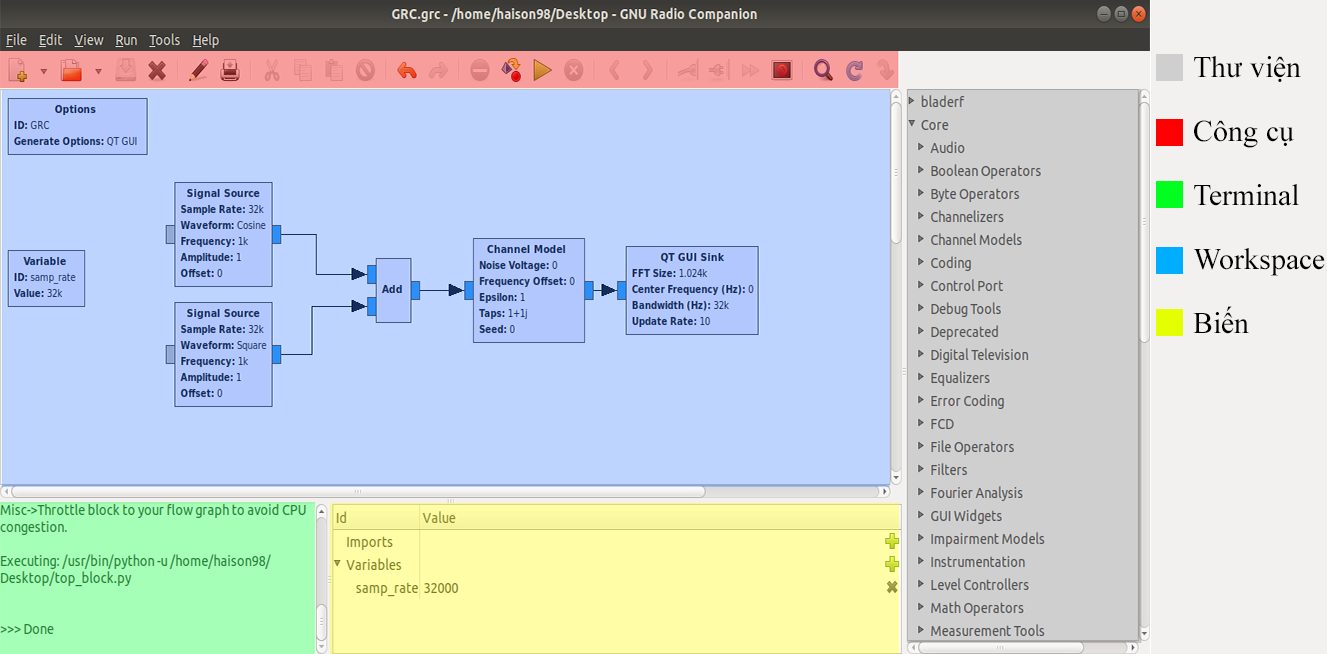
\includegraphics[width=1\linewidth]{figures/GNURadio1.png}
	\caption{Giao diện GNU Radio Companion}
	\label{fig:GNURadio}
\end{figure}

GNU Radio được viết hoàn toàn bằng ngôn ngữ C++ để đảm bảo hiệu năng, tuy nhiên người dùng vẫn có thể sử dụng Python để viết các khối do GNU Radio sử dụng SWIG để liên kết C++ với các ngôn ngữ bậc cao mà ở đây là Python. Hình \ref{fig:SWIG} mô tả cách thức vận hành của GNU Radio và cách nó liên kết với thiết bị SDR.

\begin{figure} [!htb]
	\centering
	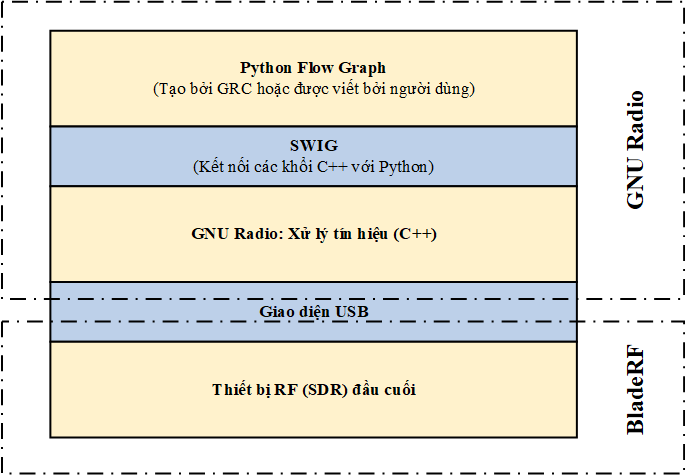
\includegraphics[width=0.9\linewidth]{figures/SWIG.png}
	\caption{Sơ đồ làm việc của GNU Radio}
	\label{fig:SWIG}
\end{figure}

Các luồng dữ liệu trong GNU Radio đi qua các khối thực thi được phân chia rõ ràng về kiểu dữ liệu như trên hình \ref{fig:colormapping} và độ dài của vector dữ liệu như hình \ref{fig:streamdata}, chỉ khi chúng khớp nhau, GRC thông báo hợp lệ thì chương trình mới có thể chạy. Điều này có được là do ngay trong việc khởi tạo khối, các thông số trên đã được định sẵn để đảm bảo việc xử lý tín hiệu là đúng với mục đích ban đầu của khối.

\begin{figure}[!h]
%\hfill
\centering
\subfigure[Mã màu của các kiểu dữ liệu]{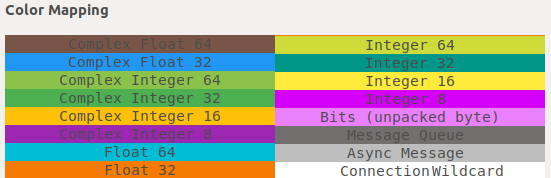
\includegraphics[width=0.9\linewidth]{figures/colormapping.png}\label{fig:colormapping}}
\hfill
\subfigure[Luồng dữ liệu qua các khối xử lý]{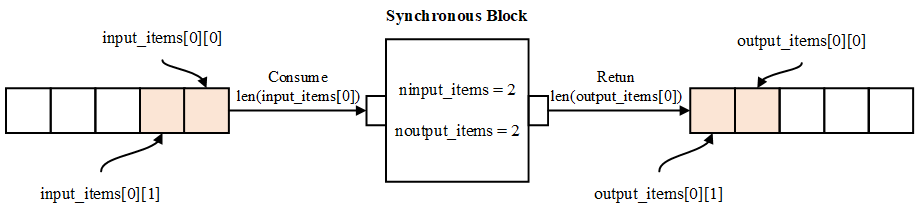
\includegraphics[width=0.9\linewidth]{figures/streamdata.png}\label{fig:streamdata}}
\hfill
\caption{Kiểu dữ liệu và xử lý tín hiệu trong GNU Radio}
\end{figure}

Đối với các nhà phát triển muốn tạo thêm các khối thực hiện các chức năng đặc biệt, GNU Radio cung cấp khả năng tương thích với cả C++ và Python. Bảng \ref{methodGNURadio} dưới đây so sánh tính năng của các phương pháp lập trình khối trong GNU Radio.

\begin{table}[!h]
	\caption{Các phương pháp sử dụng GNU Radio}
	\resizebox{1\hsize}{!} {
		\begin{tabular}{|l|l|l|}
			\hline
			\multicolumn{1}{|c|}{\multirow{2}{*}{\textbf{GNU Radio Companion}}} & \multicolumn{1}{c|}{\multirow{2}{*}{\textbf{C++}}} & \multicolumn{1}{c|}{\multirow{2}{*}{\textbf{Python}}} \\
			\multicolumn{1}{|c|}{} & \multicolumn{1}{c|}{} & \multicolumn{1}{c|}{} \\ \hline
			&  &  \\
			Dễ dàng và trực quan. & Đầy đủ các tùy chỉnh. & Đầy đủ các tùy chỉnh. \\
			&  &  \\ \hline
			&  &  \\
			\begin{tabular}[c]{@{}l@{}}Tạo flow-graph bằng cách kết nối và\\ tinh chỉnh các khối có sẵn trong GRC.\end{tabular} & Tốc độ thực thi nhanh. & \begin{tabular}[c]{@{}l@{}}Lập trình nhanh chóng\\ (Numpy, Scipy,...)\end{tabular} \\
			&  &  \\ \hline
			&  &  \\
			& Thực hiện tốt các hệ truyền thông thời gian thực. & \begin{tabular}[c]{@{}l@{}}Tốt trong việc thực hiện các\\ thực nghiệm nhanh chóng.\end{tabular} \\
			&  &  \\ \cline{2-3} 
			&  &  \\
			& Độ phức tạp và thời gian lập trình lâu. &  \\
			&  &  \\ \cline{2-2}
			&  &  \\
			& Kết nối với Python bằng SWIG. &  \\
			&  &  \\ \hline
	\end{tabular} }
	\label{methodGNURadio}
\end{table}

%\begin{figure} [!h]
%	\centering
%	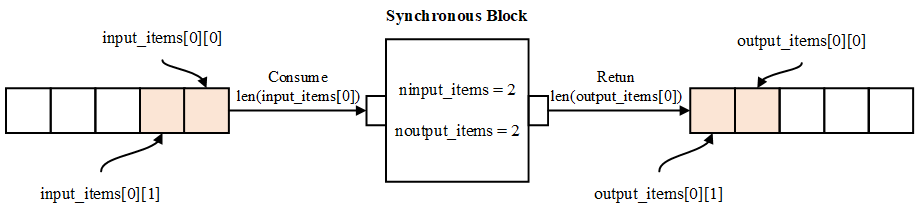
\includegraphics[width=1\linewidth]{figures/streamdata.png}
%	\caption{Luồng dữ liệu qua các khối xử lý trong GNU Radio}
%	\label{fig:streamdata}
%\end{figure}

\subsection{Thiết bị vô tuyến định nghĩa bằng phần mềm SDR}

Vô tuyến định nghĩa bằng phần mềm (Software Define Radio) là một hệ thống truyền thông vô tuyến được thực hiện chủ yếu bằng phần mềm trên máy tính cá nhân hoặc hệ thống nhúng. Một SDR cơ bản bao gồm máy tính có sound card  hoặc thiết bị chuyển đổi tương tự sang số (ADC) cùng thiết bị chuyển đổi số sang tương tự (DAC) và đầu cuối cao tần để thu phát tín hiệu, mô tả khái quát ở hình \ref{fig:structSDR}. Phần xử lý tín hiệu hầu hết được thực hiện bởi bộ xử lý đa năng (GPP) thay vì phần cứng chuyên dụng (mạch điện tử). Với thiết kế này một thiết bị SDR có thể truyền nhận được tín hiệu ở nhiều tần số,  loại điều chế khác nhau chỉ dựa trên phần mềm sử dụng.

\begin{figure} [!htb]
	\centering
	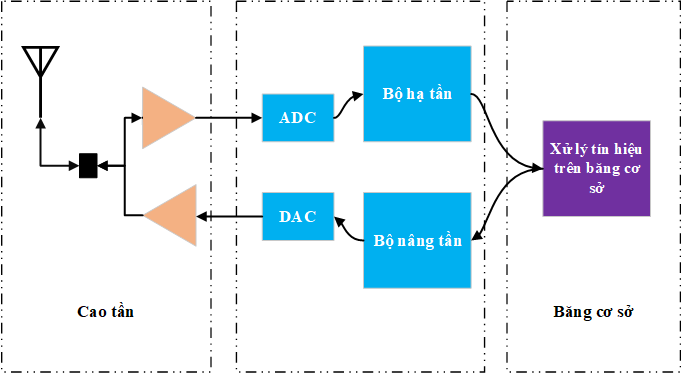
\includegraphics[width=1\linewidth]{figures/structSDR.png}
	\caption{Sơ đồ khối phần cứng hệ thống SDR}
	\label{fig:structSDR}
\end{figure}

Software Define Radio được sử dụng trong các ứng dụng quân sự \cite{Bergstrom2002} và trong viễn thông di động \cite{VanRijsbergen, Gomez-Miguelez2016}, cả hai đều có thể sử dụng nhiều giao thức vô tuyến và đáp ứng thời gian thực. Về lâu dài, SDR được mong đợi sẽ trở thành công nghệ thống trị trong truyền thông vô tuyến bằng cách kết hợp với Anten định nghĩa bằng phần mềm (Software Define Antennas) tạo thành vô tuyến nhận thức (Cognitive Radio).

Với tên ban đầu máy thu kỹ thuật số (Digital Receiver) được tạo ra vào năm 1970 bởi một nhà nghiên cứu thuộc bộ quốc phòng Hoa Kỳ, từ năm 1990 đến 1995, ứng dụng trong dự án SpeakEasy \cite{Fakhrian2012}, một chương trình cho các đài phát thanh điều khiển không quân mặt đất chiến thuật của không quân Hoa Kỳ có thể hoạt động từ 2 MHz đến 2 GHz. Thuật ngữ Software Define Radio do Stephen Blust đặt ra và đề xuất tại Modular Multifunction Information Transfer Systems năm 1996. Tiếp tục được nghiên cứu và phát triển liên tục sau đó, đến nay đã có nhiều sản phẩm thương mại SDR đã bán ra trên toàn cầu cho mục đích quân sự, nghiên cứu, giảng dạy hay ứng dụng vào sản phẩm truyền thông không dây thực tế. Có thể kể đến trong quân sự, dự án Joint Tactical Radio System (JTRS) \cite{Feickert2005} sản xuất bộ đàm cung cấp liên lạc linh hoạt và có thể tương tác, nhưng do vấn đề chi phí cao hơn so với việc sử dụng các linh kiện chuyên dụng cho một mục đích nên chưa được sử dụng rộng rãi. Tuy nhiên, tính linh hoạt của SDR có thể là chìa khóa cho truyền thông vô tuyến trong tương lai, một khi chi phí cố định để sản xuất một SDR đã giảm đủ để vượt qua chi phí thiết kế lại các hệ thống sử dụng linh kiện điện tử cho một mục đích.

\begin{figure} [!htb]
	\centering
	\includegraphics[width=0.5\linewidth]{figures/commonSDR.png}
	\caption{Các thiết bị SDR thông dụng}
	\label{fig:commonSDR}
\end{figure}

Các ứng dụng trong giảng dạy và nghiên cứu với SDR thông dụng hơn, với rất nhiều thiết bị SDR ở nhiều mức giá và mục đích khác nhau (hình \ref{fig:commonSDR}). Từ các thiết bị giá rẻ chỉ 22 \$ như DVB-T USB dongles sử dụng IC điều khiển Realtek RTL2832U, và Rafael Micro R820T làm bộ chỉnh tần số, thiết bị chỉ thực hiện chức năng thu tín hiệu, có thể hoạt động trong dải từ 500 kHz đến 1,75 GHz để thu FM, DVB-T, GSM,... Với các nghiên cứu chuyên sâu hơn Universal Software Radio Peripheral (USRP) là lựa chọn tốt với dải thu siêu cao tần lên đến 6 GHz băng thông rộng 200 MHz cùng khả năng MIMO được tích hợp sẵn.

\section{Phần cứng và phần mềm của BladeRF}

\subsection{BladeRF x115}

Trong nghiên cứu này  sử dụng các Kit SDR là BladeRF x115 của Nuand, ra mắt năm 2013, được tích hợp nhiều công nghệ mới: hỗ trợ truyền nhận đồng thời (full duplex), bộ ADC, DAC tốc độ cao, khả năng lập trình FPGA, tương thích giao diện USB 3.0, cổng kết nối mở rộng (GPIO), MIMO,... Các thông số chi tiết ở bảng \ref{parabladeRF}.

% Please add the following required packages to your document preamble:
% \usepackage[table,xcdraw]{xcolor}
% If you use beamer only pass "xcolor=table" option, i.e. \documentclass[xcolor=table]{beamer}
%\begin{table}[!htb]
%\resizebox{1\hsize}{!} {
%\begin{tabular}{lcccc}
%\hline
%\rowcolor[HTML]{FFECEA} 
%Thông Số & Nhỏ nhất & Thông thường & Lớn nhất & Đơn vị \\ \hline
%\rowcolor[HTML]{EFEFEF} 
%\multicolumn{5}{l}{\cellcolor[HTML]{EFEFEF}Thông số kỹ thuật RF} \\ \hline
%ADC/DAC Sample Rate & 0.16 &  & 40 & MHz \\ \hline
%ADC/DAC Resolution &  & 12 &  & bits \\ \hline
%VCTCXO Accuracy &  & 1 &  & ppm \\ \hline
%RF Tuning Range & 300 &  & 3 800 & MHz \\ \hline
%RF Bandwidth Filter & 1.5 &  & 28 & MHz \\ \hline
%CW Output &  & +6 &  & dBm \\ \hline
%\rowcolor[HTML]{EFEFEF} 
%\multicolumn{5}{l}{\cellcolor[HTML]{EFEFEF}Thông số kỹ thuật FPGA} \\ \hline
%Logic Elements &  &  & 114 480 & LE \\ \hline
%Embedded 18x18 Multipliers &  &  & 266 &  \\ \hline
%BRAM &  &  & 3 888 & kbits \\ \hline
%\rowcolor[HTML]{EFEFEF} 
%\multicolumn{5}{l}{\cellcolor[HTML]{EFEFEF}Thông số vật lý} \\ \hline
%Kích thước &  & 8.7 x 13.1 x 1.8 &  & cm \\ \hline
%Cân nặng &  & 80 &  & g \\ \hline
%Nhiệt độ làm việc & 0 &  & 70 & $^{\circ}$C \\ \hline
%\end{tabular} 
%}
%\caption{Thông số kỹ thuật của BladeRF x115}
%\label{parabladeRF}
%\end{table}

\begin{table}[!htb]
\caption{Thông số kỹ thuật của BladeRF x115}
\resizebox{1\hsize}{!} {
\begin{tabular}{|l|c|c|c|c|} 
\hline
\rowcolor[rgb]{1,0.925,0.918} Thông Số & Nhỏ nhất & Thông thường     & Lớn nhất & Đơn vị        \\ 
\hline
\multicolumn{5}{|l|}{{\cellcolor[rgb]{0.937,0.937,0.937}}Thông số kỹ thuật RF}                  \\ 
\hline
ADC/DAC Sample Rate                    & 0,16     &                  & 40       & MHz           \\ 
\hline
ADC/DAC Resolution                     &          & 12               &          & bits          \\ 
\hline
VCTCXO Accuracy                        &          & 1                &          & ppm           \\ 
\hline
RF Tuning Range                        & 300      &                  & 3 800    & MHz           \\ 
\hline
RF Bandwidth Filter                    & 1,5      &                  & 28       & MHz           \\ 
\hline
CW Output                              &          & +6               &          & dBm           \\ 
\hline
\multicolumn{5}{|l|}{{\cellcolor[rgb]{0.937,0.937,0.937}}Thông số kỹ thuật FPGA}                \\ 
\hline
Logic Elements                         &          &                  & 114 480  & LE            \\ 
\hline
Embedded 18x18 Multipliers             &          &                  & 266      &               \\ 
\hline
BRAM                                   &          &                  & 3 888    & kbits         \\ 
\hline
\multicolumn{5}{|l|}{{\cellcolor[rgb]{0.937,0.937,0.937}}Thông số vật lý}                       \\ 
\hline
Kích thước                             &          & 8,7 x 13,1 x 1,8 &          & cm            \\ 
\hline
Cân nặng                               &          & 80               &          & g             \\ 
\hline
Nhiệt độ làm việc                      & 0        &                  & 70       & $^{\circ}$C   \\
\hline
\end{tabular}
}
\label{parabladeRF}
\end{table}

Cấu hình bên trong của BladeRFx115 biểu diễn trên hình \ref{fig:structbladeRF}, các thành phần chính bao gồm: 

\begin{figure} [!htb]
	\centering
	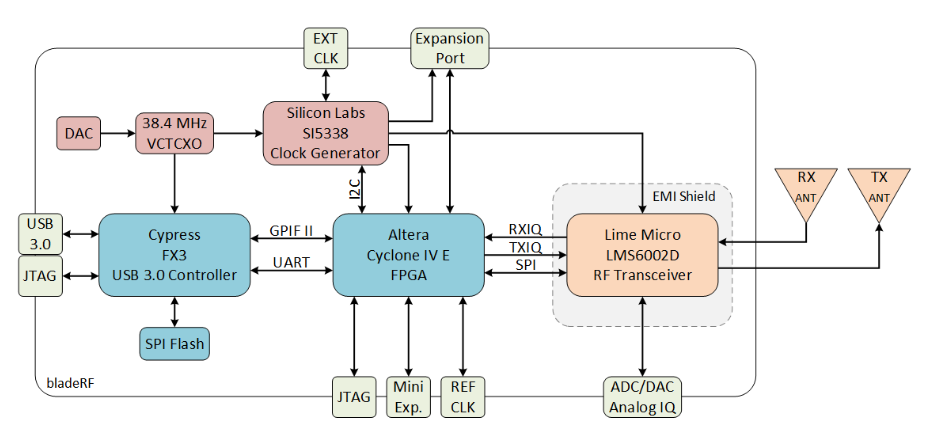
\includegraphics[width=1\linewidth]{figures/structbladeRF.png}
	\caption{Cấu hình của BladeRF x115}
	\label{fig:structbladeRF}
\end{figure}

\begin{itemize}
	\item	Altera Cyclone IV EP4CE15 FPGA: thành phần xử lý trung tâm của BladeRF, có thể lập trình lại qua cổng JTAG.
	\item 	Lime Micro LMS6002D RF Transceiver: IC thu phát cao tần có thể lập trình, hoạt động trong dải 300 MHz đến 3,8 GHz, trên cả băng tần được cấp phép và không được cấp phép và với bất cứ tiêu chuẩn truyền thông không dây nào. Các bộ ADC, DAC 12 bits truyền trực tiếp mẫu đến FPGA. Tích hợp sẵn LNA, PA, bộ trộn TX/RX, bộ lọc TX/RX, ...
	\item   Cypress FX3 USB 3.0 Controller: bộ điều khiển ngoại vi USB 3.0 tốc độ cao băng thông 5 Gbps, có cấu hình qua $\mathrm{GPIF^{TM} II}$. Là cầu nối giao tiếp giữa BladeRF và máy tính hay các thiết bị ngoại vi khác như SPI Flash.
	\item   SPI Flash: IC MX25U3235EM2I-10G cung cấp 32 Mb bộ nhớ Flash.
	\item   Silicon Labs Si5338 Clock Generator: bộ tạo xung đồng hồ chuẩn cho toàn BladeRF, giao tiếp với FPGA qua chuẩn I2C.
	\item 	VCTCXO: bộ tạo dao động tinh thể để bù cho nhiệt độ, được hiệu chuẩn ở mức sai số dưới 1 Hz trong 38,4 MHz.
	%\item 	SPI Flash: sử dụng IC MX25U3235EM2I-10G cung cấp 32Mb bộ nhớ Flash.
	\item 	Expansion port, EXT CLK, Mini Exp, REF CLK, JTAG, ADC/DAC Analog IQ: các cổng mở rộng để phục vụ từng mục đích chuyên biệt cho BladeRF.
\end{itemize}

\subsection{Phần mềm của BladeRF}

Dữ liệu đầu ra từ BladeRF truyền về máy tính là các mẫu IQ được lấy mẫu như hình \ref{fig:IQsample}, lưu ở chuẩn SC16Q11, khi đưa vào các khối trong GNU Radio sẽ chuyển đổi sang Complex Float32.

\begin{figure} [!h]
	\centering
	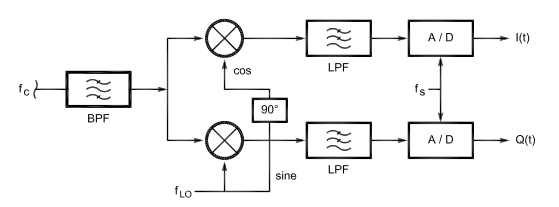
\includegraphics[width=1\linewidth]{figures/IQsample.png}
	\caption{Lấy mẫu IQ}
	\label{fig:IQsample}
\end{figure}

Để sử dụng dữ liệu đầu ra của BladeRF cho công việc xác định hướng sóng đến, cần phải viết thêm những khối OTT (Out Of Tree Modules) vào GNU Radio để đảm nhiệm việc xử lý tín hiệu. Có nhiều cách để tạo một khối OTT trên GNU Radio, đơn giản nhất là sử dụng ngay Python Block là một khối trong thư viện của GNU Radio, cho phép lập trình một khối mới ngay lập tức với ngôn ngữ Python, hình \ref{fig:pythonblock} là khối Python Block trên GRC và mã lập trình có sẵn bên trong khối. Tuy nhiên hạn chế ở hiệu năng và không thể tùy biến được nhiều và sâu cho khối, vì vậy chỉ nên sử dụng khi kiểm tra nhanh thuật toán. Một cách nữa do nhà phát hành cung cấp chính thức cho các nhà phát triển đó là công cụ gr\_modtool.
\newpage
\begin{figure}[!htb]
%\hfill
\subfigure[Khối Python Block trên GRC]{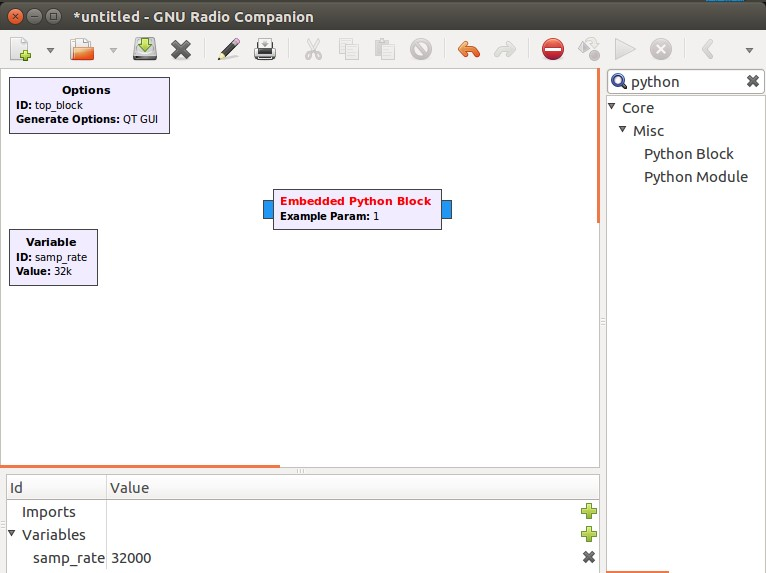
\includegraphics[width=0.49\linewidth]{figures/pythonblock.jpg}}
\hfill
\subfigure[Lập trình cho khối Python Block]{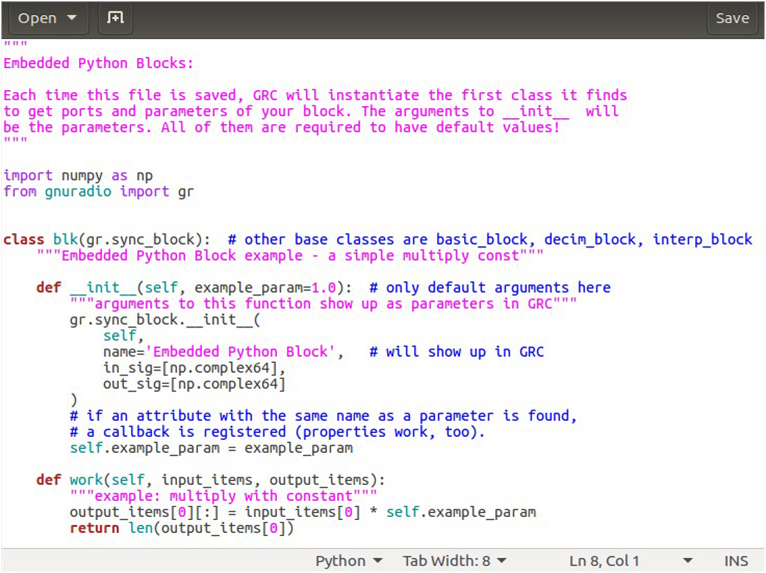
\includegraphics[width=0.49\linewidth]{figures/pythonblock2.jpg}}
\hfill
\caption{Tạo khối với Python Block trên GNU Radio}
\label{fig:pythonblock}
\end{figure}

Công cụ gr\_modtool được tích hợp sẵn vào GNU Radio từ năm 2010, sử dụng để tạo sẵn template các khối OTT với chức năng đa dạng cho người dùng, giúp bỏ qua các bước phải lặp đi lặp lại như: tạo các mã soạn sẵn, sửa makefile, ... Hỗ trợ lập trình khối cho GNU Radio với ngôn ngữ C++ và Python với liên kết bằng SWIG tích hợp sẵn, việc cài đặt các khối sau khi lập trình được thực  hiện tự động bằng CMAKE, hoàn toàn phù hợp cho cả người mới bắt đầu vào các mục đích nghiên cứu chuyên sâu. Hình \ref{fig:grmodtool} ví dụ một Module tạo bằng gr\_modtool chứa nhiều thư mục và file đã tạo sẵn, một Module có thể chứa nhiều khối OTT.

\begin{figure} [!h]
	\centering
	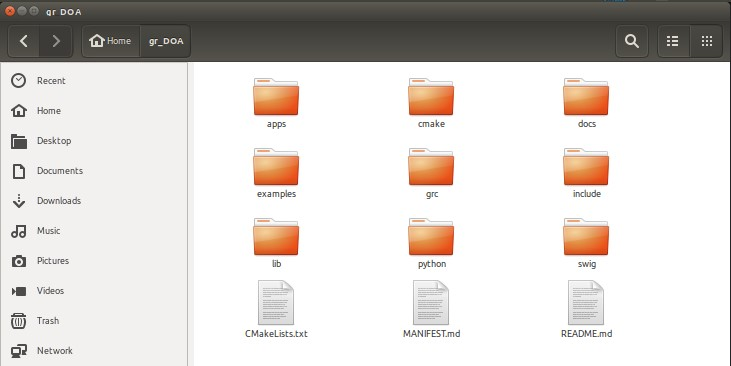
\includegraphics[width=1\linewidth]{figures/grmodtool.jpg}
	\caption{Module tạo bằng gr\_modtool}
	\label{fig:grmodtool}
\end{figure}

Tiếp theo, cần xác định loại khối cho các mục đích khác nhau, dưới đây là 4 loại khối được GNU Radio cung cấp:
\renewcommand{\labelitemi}{$-$}
\begin{itemize}
	\item Synchronous Blocks: Số mẫu đầu vào và đầu ra của khối là bằng nhau (1/1).
	\item Decimation Blocks: Cứ N mẫu đầu vào thì có 1 mẫu đầu ra (N/1).
	\item Interpolation Blocks: Cứ 1 mẫu đầu vào thì có M mẫu đầu ra (1/M).
	\item General Blocks: Tùy chỉnh tỷ lệ số mẫu đầu vào và đầu ra (N/M).
\end{itemize}

Việc cài đặt khối vào GNU Radio sau khi lập trình xong cũng rất đơn giản do sử dụng CMAKE, sau khi đã cài đặt, các khối OTT sẽ xuất hiện trong hộp thoại của GRC, dễ dàng chọn, tùy chỉnh thông số và kết nối với nhau.

\section{Triển khai hệ thống xác định hướng sóng đến trên hệ BladeRF}

Trên thực tế, việc xây dựng một hệ thống gồm nhiều thiết bị SDR mà ở đây là BladeRF để phục vụ cho việc xác định hướng sóng đến, yêu cầu hệ thu cần phải được đồng bộ hoàn toàn với nhau trước khi sử dụng dữ liệu của SDR để ước lượng DOA.

Trong phần này, để phù hợp với thực tế về số lượng SDR và phần cứng có sẵn, mảng anten thu sẽ chỉ gồm 2 phần tử BladeRF. Các bước đồng bộ dưới đây vẫn áp dụng được cho hệ nhiều phần tử BladeRF, tuy nhiên sẽ cần thêm các phần cứng chuyên dụng: bộ chia bù công suất, bộ chia giữ nguyên độ lệch pha, máy phát xung chuẩn. Chi tiết như sau: 

Không giống như dữ liệu lý tưởng khi mô phỏng, dữ liệu thực tế từ hệ SDR sẽ gặp các vấn đề cần phải được xử lý: xung đồng hồ chủ khác nhau; $\textrm{DC}_\textrm{offset}$ và cân bằng mẫu IQ cho các từng thiết bị SDR; việc truyền/nhận dữ liệu từ GNU Radio trên máy tính đến các SDR qua cổng USB thường không được thực hiện đồng thời, dẫn đến hiện tượng các các SDR bắt đầu chạy và gửi mẫu về ở các thời gian khác nhau, gây ra trễ mẫu ($\textrm{sample}_{\textrm{offset}}$) trên dữ liệu mảng thu; sai số trong thời gian lấy mẫu (\textrm{time sampling}); độ lệch pha giữa 2 tín hiệu ($\textrm{phase}_{\textrm{offset}}$) ở trạng thái ban đầu; cùng với vấn đề sai số ($f_{\textrm{offset}}$) trong tần số thu của từng SDR. Khi hiệu chỉnh hoàn tất, hệ SDR đồng bộ thì mới sử dụng được dữ liệu của chúng cho thuật toán DOA để ước lượng hướng sóng đến. Bảng \ref{tab:issue} bên dưới nêu ra các phương pháp được sử dụng để đồng bộ hệ BladeRF trong khóa luận và đưa thêm một số phương pháp khác có thể áp dụng cho các loại SDR khác.


\begin{sidewaystable}[htbp]
\centering
\caption{Phương pháp đồng bộ hệ BladeRF được sử dụng trong khóa luận}
%\begin{table}[!h]
\begin{tabular}{|l|l|l|}
	\hline
	\rowcolor[HTML]{FFECEA} 
	\multicolumn{1}{|c|}{\cellcolor[HTML]{FFECEA}\textbf{Vấn đề đồng bộ}} & \multicolumn{1}{c|}{\cellcolor[HTML]{FFECEA}\textbf{Phương pháp giải quyết được sử dụng}} & \multicolumn{1}{c|}{\cellcolor[HTML]{FFECEA}\textbf{Các phương pháp khác}} \\ \hline
	\begin{tabular}[c]{@{}l@{}}$\mathrm{DC}_\mathrm{offset}$\\ và cân bằng mẫu IQ\end{tabular} & \begin{tabular}[c]{@{}l@{}}Hiệu chỉnh bằng tính năng trong thư viện của BladeRF\\ có sẵn, và khối DC Blocker trên GNU Radio.\end{tabular} &  \\ \hline
	Xung đồng hồ chủ & \begin{tabular}[c]{@{}l@{}}Chia sẻ xung đồng hồ chủ (CLK) qua chân\\ SMB (System Management Bus) trên BladeRF.\end{tabular} & \begin{tabular}[c]{@{}l@{}}$\ast$ Sử dụng thêm phần cứng:\\ $-$ Silicon Labs SI5338 Clock Generator Evaluation Board, \\ sử dụng cùng loại IC SI5338 như trên BladeRF cho phép chia xung\\ tối đa đến 8 thiết bị khác.\end{tabular} \\ \hline
	$\mathrm{Sample}_\mathrm{offset}$ & Phân tích tương quan chéo của tín hiệu mảng thu. & \begin{tabular}[c]{@{}l@{}}$\ast$ Sử dụng thêm phần cứng: \\ $-$ Noise Source Card và tương quan chéo của nhiễu Gauss,\\ chuyển đổi qua lại giữa Noise Source Card và RF từ anten \\ qua giao tiếp I2C \cite{kerberos}.\\ $-$ Sử dụng chân MIMO có trên các SDR cao cấp (BladeRF, USRP), \\ trên BladeRF x115: chân J71 pin 4.\\ \\ $\ast$ Sử dụng phần mềm:\\ $-$ Sử dụng một kênh tham chiếu cố định (FM, DVB-T, GSM, ...)\\ được thực hiện trong dự án Multi-RTL: sử dụng kênh BCCH của \\ GSM để đồng bộ \cite{multi-rtl}.\end{tabular} \\ \hline
	$\textrm{Time sampling}$ & Do đã chia sẻ CLK nên bỏ qua công đoạn này. & \begin{tabular}[c]{@{}l@{}}$\ast$ Sử dụng thêm phần cứng:\\ $-$ Sử dụng chân J71 pin 4, tính năng Trigger trong $bladeRF-cli$\\ khóa xung lấy  mẫu của các BladeRF với nhau.\end{tabular} \\ \hline
	$f_\mathrm{offset}$ & Công cụ kalibrate-bladeRF do nhà sản xuất cung cấp. & \begin{tabular}[c]{@{}l@{}}$\ast$ Sử dụng thêm phần cứng:\\ $-$ Cấp tín hiệu chuẩn: 1 xung/giây hoặc 10 MHz ở mức điện áp 1,8 V \\ qua chân J71 pin 1 để hiệu chỉnh VCTCXO.\end{tabular} \\ \hline
	$\mathrm{Phase}_\mathrm{offset}$ & \begin{tabular}[c]{@{}l@{}}Sử dụng thuật toán MUSIC tìm độ lệch pha\\ giữa 2 tín hiệu.\end{tabular} & \begin{tabular}[c]{@{}l@{}}$\ast$ Sử dụng thêm phần cứng:\\ $-$ Sử dụng tín hiệu từ máy phát chuẩn như ở \cite{TravisFCollins}, cấp đến các SDR,\\ ước lượng độ lệch pha qua công thức: \\ \hspace{3cm} $\phi = tan^{-1} \left (\frac{Im (x(k))}{Re(x(k))} \right )$\\  với $Re$ và $Im$ lần lượt là phần thực và ảo của mẫu IQ. Sau đó, \\ bù thêm pha cho tín hiệu trễ pha: \\ \hspace{3cm} $\Delta \phi = \phi_1 - \phi_0 $\\ $ \hspace{3.2cm} \hat{\mathbf{x}}_1 = \mathbf{x}_1  e^{j \Delta \phi}$\end{tabular} \\ \hline
\end{tabular}
%\end{table}
\label{tab:issue}
\end{sidewaystable}
\newpage
Chi tiết các bước và kết quả đồng bộ hệ BladeRF x115 như sau:

\begin{itemize}
	\item[$\ast$] \textbf{Đồng bộ xung đồng hồ giữa các thiết bị SDR mảng thu}
\end{itemize}

Việc đầu tiên cần làm với một hệ sử dụng nhiều SDR, hay các hệ truyền thông khác, đó là phải chia được xung đồng hồ chủ trên một thiết bị, chia cho các thiết bị còn lại, đảm bảo chắc chắn rằng chúng chạy trên cùng một xung đồng hồ. Với BladeRF, điều này đã được nhà sản xuất tích hợp sẵn, với cổng SMB (System Management Bus) là chân J62 trên mạch hay \textit{EXT CLK} trong hình \ref{fig:structbladeRF}. Hình \ref{fig:clk} và \ref{fig:shareclk} lần lượt là xung đồng hồ tham chiếu của BladeRF chủ, và xung đồng hồ tham chiếu sau khi chia cho một BladeRF khác. 

Thông thường, với thiết lập trong \textit{bladeRF-cli} (client điều khiển của BladeRF) cổng SMB cho phép xuất xung tham chiếu (REF CLK) ở tần số 38,4 MHz, điện áp $V_{pp}$ = 3,9 V, chỉ đủ để chia cho 1 BladeRF khác, do khi hao hụt công suất mỗi khi kết nối thêm BladeRF, yêu cầu mức điện áp tối thiểu của REF CLK ở đầu vào là 3,3 V. Vì vậy để sử dụng được nhiều BladeRF trong mảng thu hơn, bắt buộc phải cần có thêm bộ chia xung bù công suất, hoặc máy phát xung chuẩn.

\begin{figure} [!h]
	\centering
	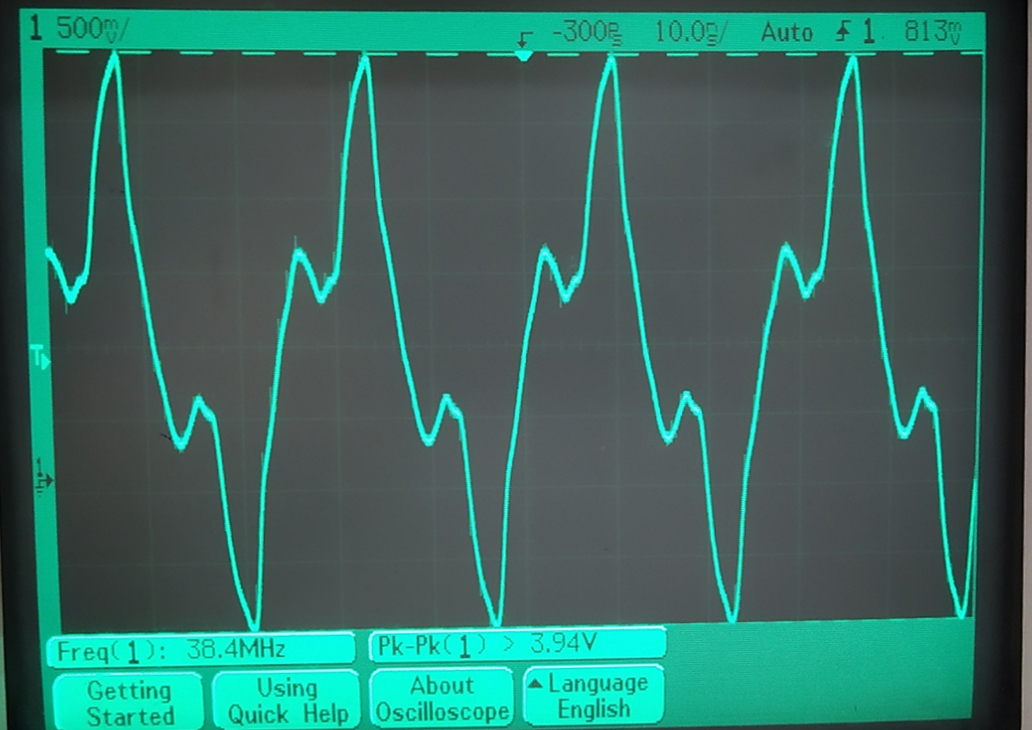
\includegraphics[width=0.7\linewidth]{figures/clk.jpg}
	\caption{Xung đồng hồ tham chiếu đầu ra của BladeRF}
	\label{fig:clk}
\end{figure}
\begin{figure} [!h]
	\centering
	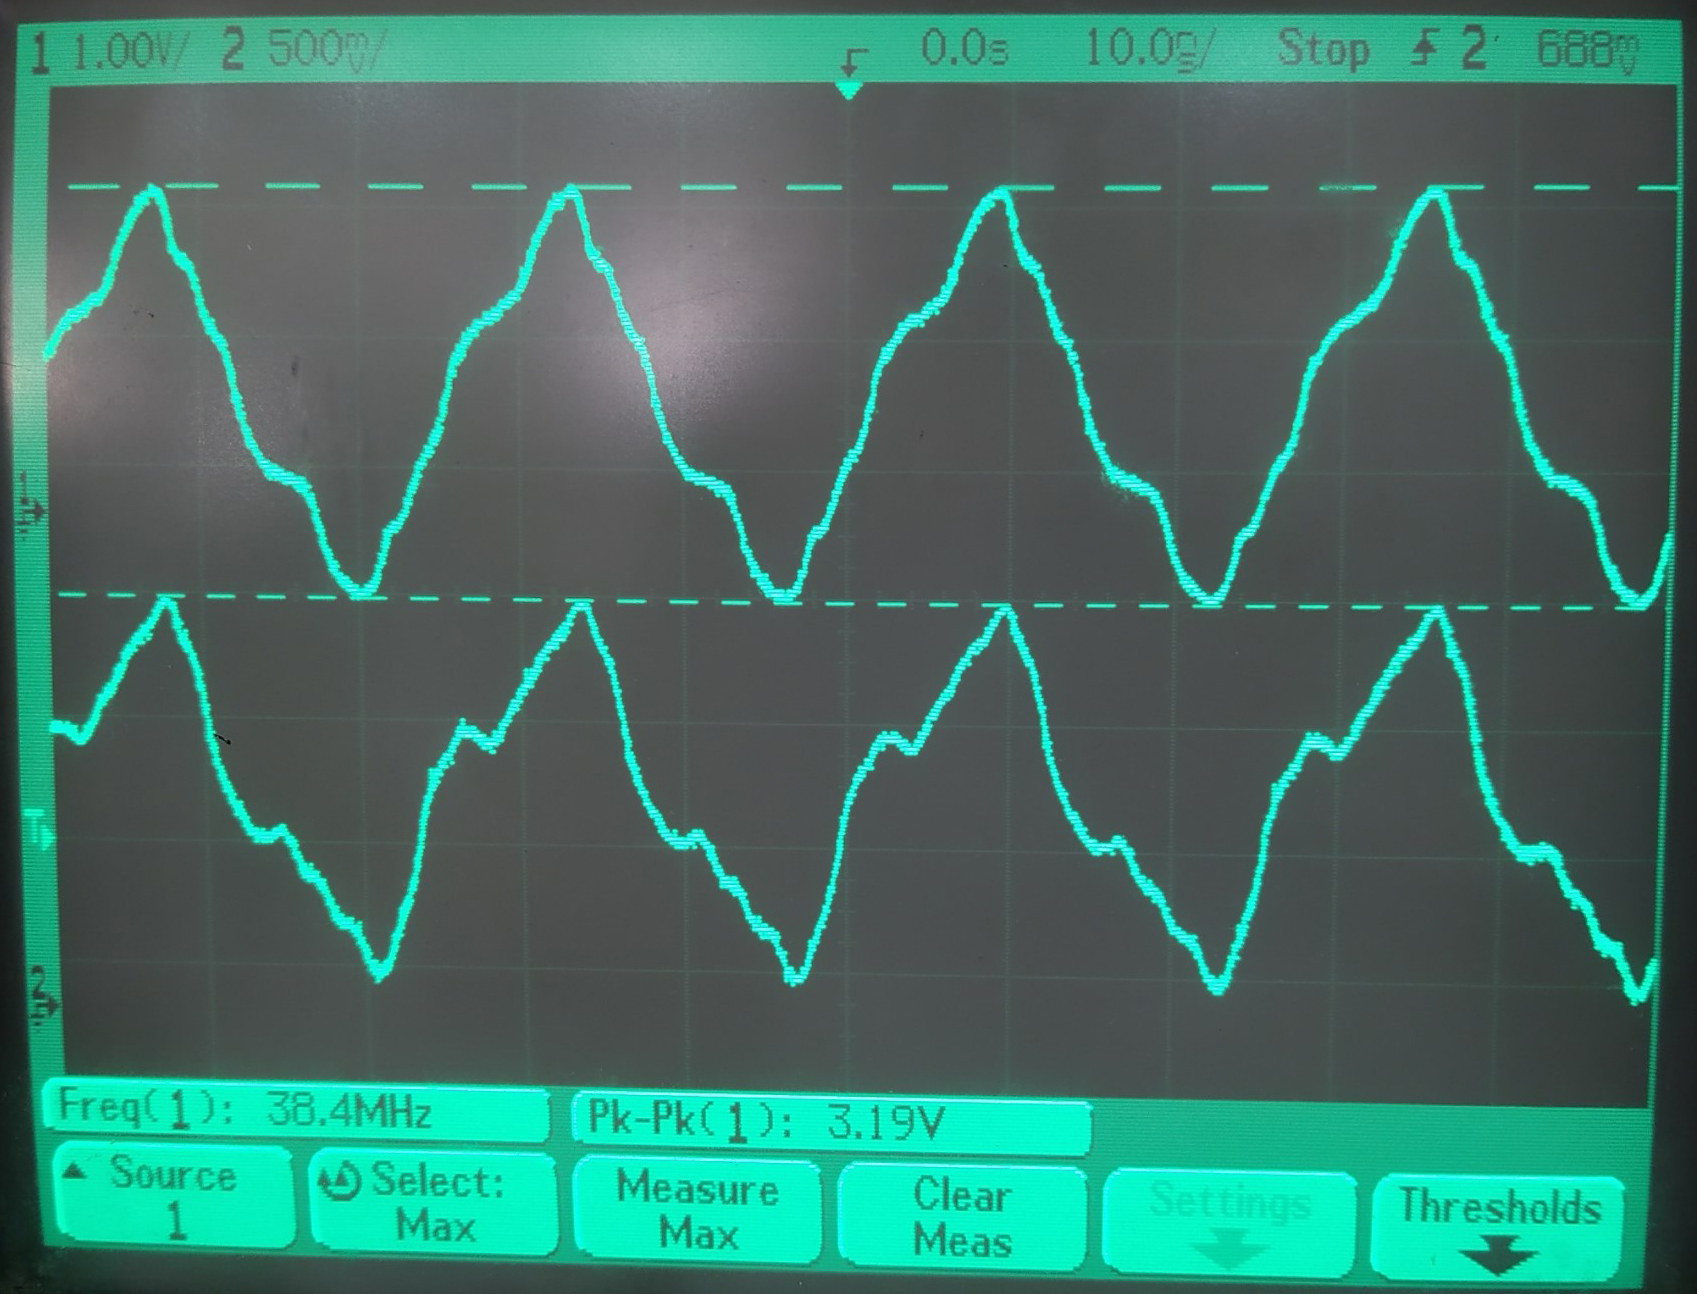
\includegraphics[width=0.7\linewidth]{figures/shareclk.jpg}
	\caption{Xung đồng hồ tham chiếu được chia sẻ}
	\label{fig:shareclk}
\end{figure}

\newpage

\begin{itemize}
	\item[$\ast$] \textbf{$\textbf{Hiệu chỉnh } \textbf{f}_{\textbf{offset}}$}
\end{itemize} 

$f_{\textrm{offset}}$ hay chính xác hơn là tần số sóng mang offset CFO (Carrier Frequency Offset), luôn tồn tại khi LO (Local Oscillator) chịu ảnh hưởng bởi nhiễu điện, chênh lệnh nhiệt độ, ... Những độ lệch này có thể tạo ra $f_{\textrm{offset}}$ và $\textrm{phase}_\textrm{offset}$ ngẫu nhiên. Trên các SDR thương mại, các thông số này đã được tính toán, và được bù lại bởi VCTCXO với độ chính xác biểu thị bởi thông số PPM (Parts Per Million). Ví dụ như BladeRF được cân chỉnh ở mức 1 PPM ở nhà máy thì $f_{\textrm{offset}}$ tối đa nếu phát/thu tín hiệu ở tần số sóng mang 923 MHz tương đương:
\begin{equation}
f_{\mathrm{offset  max}} = \frac{f_c \times\textrm{ PPM}}{10^6} = \frac{923\times 10^6 \times 1}{10^6} = 923 \textrm{ Hz}
\end{equation}

923 Hz là khá lớn, để giảm đi sai số này, nhà sản xuất cung cấp công cụ kalibrate-bladeRF \cite{kali}, cho phép người dùng sử dụng tín hiệu từ 1 kênh FCCH (Frequency Correction Channel) đường xuống từ trạm cơ sở GSM ở gần để hiệu chỉnh lại VCTCXO có thể xuống mức 0,014 PPM, tương đương với việc sai số 923 Hz như trên có thể giảm xuống 10 Hz. Kết quả thực tế như trên hình \ref{fig:freqcal} và \ref{fig:freqanly}, sau khi hiệu chỉnh kết quả thu được sai số chỉ 5 Hz ở 923 MHz và độ lệch $\Delta f_{\mathrm{offset}} = 20\textrm{ Hz}$.
\begin{figure} [!h]
	\centering
	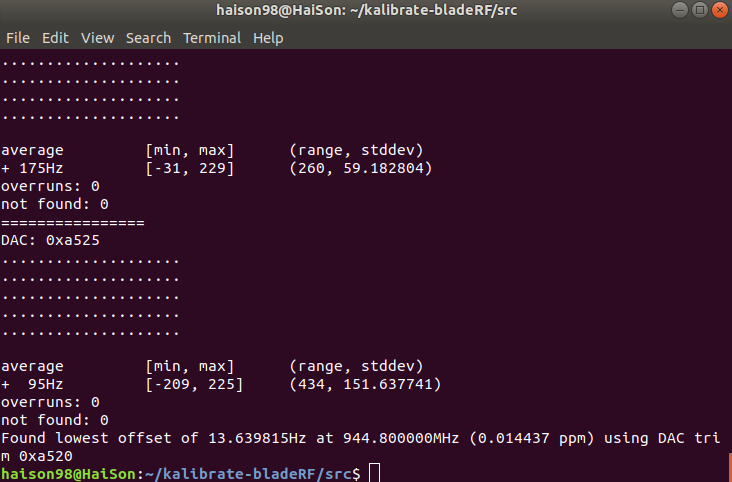
\includegraphics[width=0.85\linewidth]{figures/freqcal.png}
	\caption{Kết quả cân chỉnh tần số với kalibrate-bladeRF}
	\label{fig:freqcal}
\end{figure}

%Ngoài phương pháp sử dụng phần mềm, BladeRFx115 cung cấp cổng J71 pin 1 để người dùng sử dụng máy phát tín hiệu chuyên dụng tự hiệu chỉnh VCTCXO bằng tín hiệu 1 xung/giây, hoặc 10 MHz ở mức điện áp 1,8 V.

\begin{figure} [!ht]
	\centering
	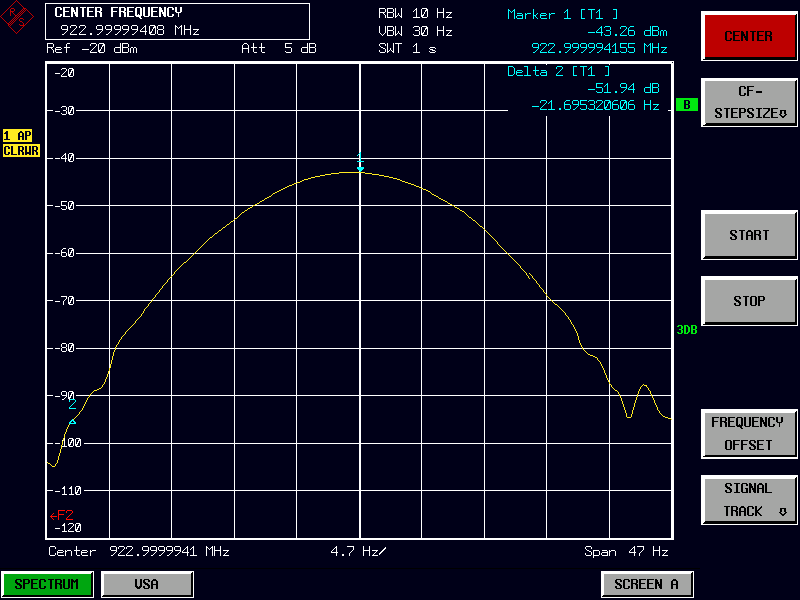
\includegraphics[width=0.85\linewidth]{figures/freqanly.png}
	\caption{Kết quả thu được trên máy phân tích phổ}
	\label{fig:freqanly}
\end{figure}

\begin{itemize}
	\item[$\ast$] \textbf{Hiệu chỉnh $\textbf{DC}_{\textbf{offset}}$ và cân bằng  mẫu IQ}
\end{itemize}

 Do được thiết kế như một bộ nhận chuyển đổi trực tiếp (Direct-conversion receiver) hay bộ nhận không có tần số trung gian (zero-IF receiver) nên trong kết quả mẫu đầu ra từ BladeRF, khi được đưa lên phổ FFT, sẽ luôn có một đỉnh phổ ở tần số trung tâm 0 Hz biểu diễn cho điện áp DC, hiện tại BladeRF chưa có phần cứng để bù vào phần DC này nên chỉ có thể giảm thiểu về mức thấp.

Nhà sản xuất đã tích hợp sẵn việc hiệu chỉnh trong thư viện của BladeRF, chi tiết có tại \cite{Dccali}. Ngoài việc hiệu chỉnh trên phần cứng BladeRF, cần sử dụng thêm khối DC Blocker trên GNU Radio để loại bỏ hoàn toàn thành phần DC.

\begin{itemize}
	\item[$\ast$] \textbf{Hiệu chỉnh $\textrm{sample}_{\textbf{offset}}$}
\end{itemize} 

Trong khóa luận này sẽ sử dụng tương quan chéo của tín hiệu thu để ước lượng số mẫu trễ gây ra bởi phần cứng BladeRF và USB. Đây là phương pháp có tính linh hoạt cao, có thể đồng bộ lượng mẫu đầu vào lớn (chục triệu mẫu), tuy nhiên bị giới hạn độ chính xác bởi môi trường truyền.

Tương quan chéo biểu hiện cho sự giống nhau của 2 tín hiệu, trong trường hợp này, có thể được dùng để ước lượng trễ mẫu giữa tín hiệu thu được từ 2 BladeRF bằng việc sử dụng một tín hiệu tham chiếu $\mathbf{x}(t)$. Trước hết, công thức toán học của tương quan chéo được ký hiệu $\mathbf{x_1 \star x_2}$ giữa 2 tín hiệu phức \cite{Bracewell1978}:
\begin{equation}
\begin{split}
&\mathbf{x}(t): \textrm{Tín hiệu cơ sở}\\
&\mathbf{x}_1(t) =\mathbf{x}(t)\\
&\mathbf{x}_2(t) =\mathbf{x}(t - T) \\
&\mathbf{x_1 \star x_2}(\tau) \triangleq \int_{-\infty}^{+\infty} \mathbf{x}_{1}^{*} (t) \mathbf{x}_{2} (t + \tau) dt \\
&T =\textrm{argmax}(\mathbf{x_1 \star x_2})
\end{split}
\end{equation}
với $^*$ là ký hiệu của liên hợp phức, chỉ có nghĩa khi $\mathbf{x}_1$ là số phức, $T$  là thời gian trễ giữa 2 tín hiệu. Rời rạc công thức tương quan chéo (2.2) để áp dụng cho các mẫu:
\begin{equation}
\mathbf{x_1 \star x_2}(n) = \sum_{m = -\infty}^{\infty} \mathbf{x}^*_1 (m) .\mathbf{x}_2 (m + n)
\end{equation}
tương tự thì số mẫu trễ tương ứng là $n = \mathrm{argmax(\mathbf{x_1 \star x_2})}$. Trên hình \ref{fig:xcorr} là ví dụ về việc sử dụng tương quan chéo của nhiễu Gauss để tìm độ trễ mẫu do phần cứng gây ra, được mô phỏng là 100 mẫu. 
\begin{figure} [!h]
	\centering
	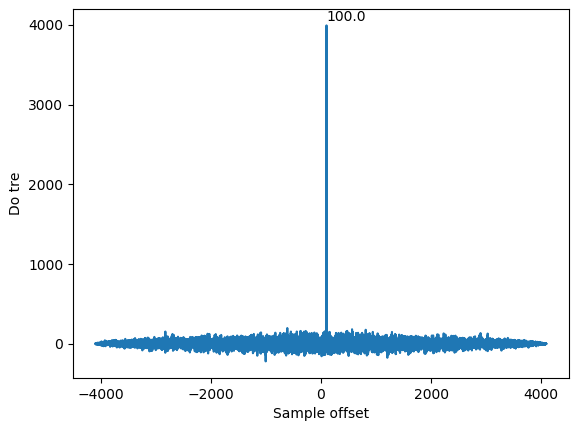
\includegraphics[width=0.8\linewidth]{figures/xcorr.png}
	\caption{Tương quan chéo của 2 nhiễu Gauss}
	\label{fig:xcorr}
\end{figure}

Cũng sử dụng tính tương quan của tín hiệu để tìm độ trễ, tuy nhiên thay vì tính toán ngay trên miền thời gian, việc chuyển sang miền tần số sẽ giúp giảm đáng kể lượng tính toán cần thiết do sử dụng khối FFT trên GNU Radio hỗ trợ chia đa luồng xử lý. Sử dụng các phép biến đổi  FFT, IFFT để tính toán trễ giữa hai tín hiệu \cite{Nentwig2016}. Áp dụng trên GNU Radio, với các khối có sẵn FFT, IFFT, Multipy Conjugate, dữ liệu đầu vào là tín hiệu được điều chế tần số băng hẹp (Narrow band FM - NBFM) được chia thành 2 nguồn, nguồn đầu tiên bị trễ 1000 mẫu so với nguồn thứ 2, lưu đồ tương ứng trên GNU Radio như hình \ref{fig:fft} và kết quả đầu ra biểu diễn qua QT GUI trên hình \ref{fig:dvb-t2} với vị trí đỉnh phổ đúng bằng số lượng trễ mô phỏng.
\begin{equation}
\begin{split}
&\mathbf{x}_1(t) \Leftrightarrow \mathbf{x}_1(f)\\
&\mathbf{x}_2(t) \Leftrightarrow \mathbf{x}_2(f)\\
&\mathbf{x_1 \star x_2} (\tau) \Leftrightarrow \mathbf{x_1 \star x_2}(f)\\
&\mathbf{x_1 \star x_2}(f) = \mathbf{x}_1^{*}(f) \mathbf{x}_2(f)
\end{split}
\end{equation}
\begin{figure}[!h]
%\hfill
\centering
\subfigure[Flow-graph mô phỏng ước lượng độ trễ giữa các đầu vào]{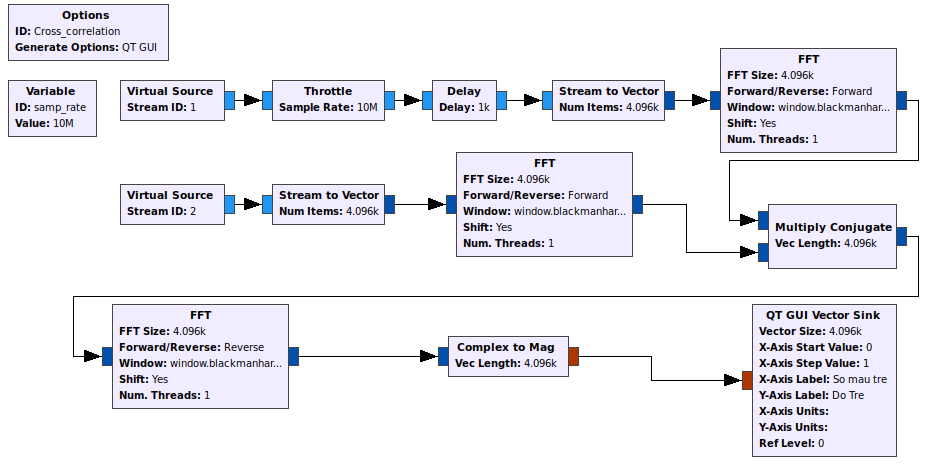
\includegraphics[width=1\linewidth]{figures/fft.png}\label{fig:fft}}
\hfill
\subfigure[Tương quan chéo của tín hiệu đầu vào]{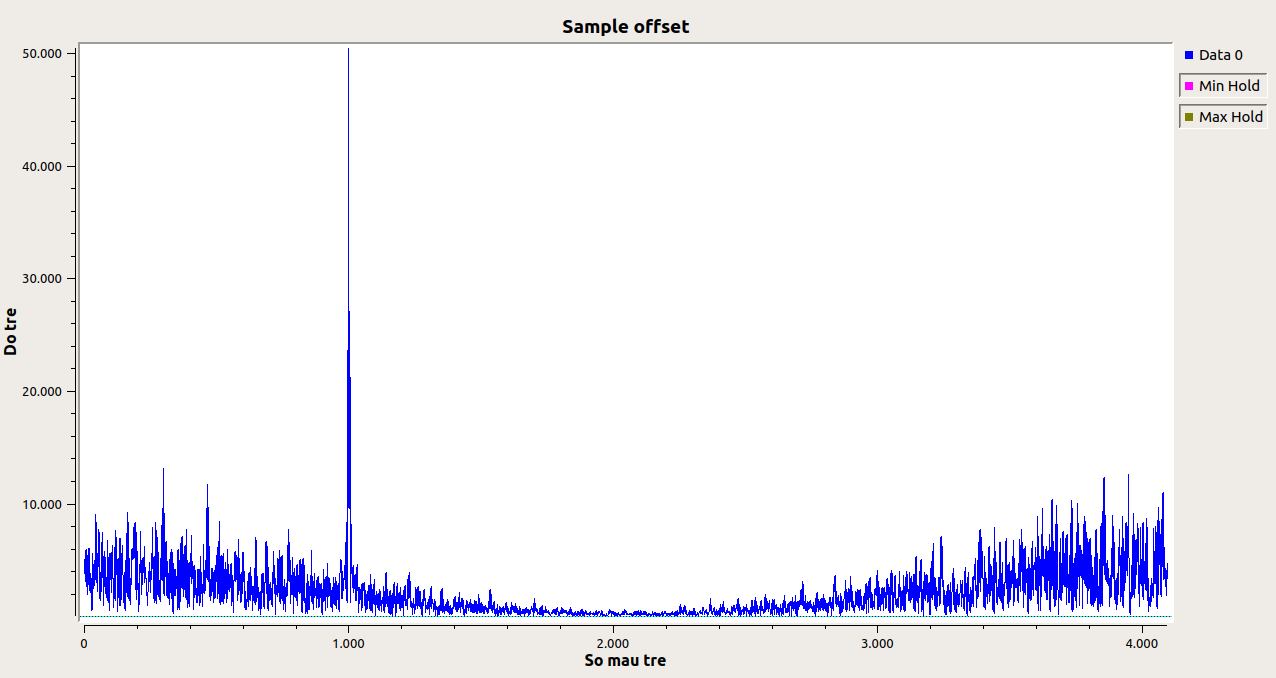
\includegraphics[width=1\linewidth]{figures/dvb-t2.png}\label{fig:dvb-t2}}
\hfill
\caption{Xác định độ trễ mẫu trên GNU Radio}
\end{figure}

Sau khi đã xác định được số mẫu trễ, sử dụng khối Delay, trễ mẫu của khối nguồn đang chạy nhanh đi một lượng $\mathrm{argmax[\mathbf{x_1 \star x_2}(f)]}$.  Flow-graph \ref{fig:fft} được viết gọn vào một khối duy nhất Sample Offset như hình \ref{fig:sample_offset} để tiện cho việc xử lý, $\textrm{sample}_\textrm{offset}$ được lưu vào một biến và phản hồi lại về đầu vào để  căn chỉnh dữ liệu khớp với nhau về mặt thời gian sẵn sàng cho các  khối xử lý tiếp theo trong GNU Radio.

\begin{figure}[!h]
%\hfill
\subfigure[Ước lượng $\textrm{sample}_\textrm{offset}$ ]{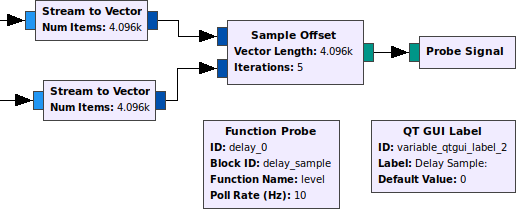
\includegraphics[width=0.6\linewidth]{figures/sample_offset.png}}
\hfill
\subfigure[Phản hồi  $\textrm{sample}_\textrm{offset}$]{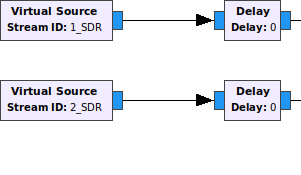
\includegraphics[width=0.35\linewidth]{figures/sample_offset_fb.png}}
\hfill
\caption{Ước lượng và phản hồi hiệu chỉnh $\textrm{sample}_\textrm{offset}$}
\label{fig:sample_offset}
\end{figure}

Nhược điểm của phương pháp này: nếu tín hiệu đầu vào có tính tương quan cao, kết quả đầu ra sẽ không chính xác tùy thuộc vào sự tương quan đó, mô phỏng cùng với kết quả mô phỏng của vấn đề này được trình bày trong mục 3.1.2 tại bảng 3.1 và 3.2; nếu độ trễ mẫu quá lớn, thông thường lớn hơn 1/2 số mẫu đầu vào khối FFT thì không thể tìm được độ trễ của các nguồn. Vì vậy, số lượng phần tử được đưa vào FFT có thể nâng lên đến hàng trăm nghìn phần tử để chắc chắn rằng thu được độ trễ khớp, nhưng để giảm thiểu tính toán, chỉ cần thực hiện hiệu chỉnh $\textrm{sample}_\textrm{offset}$ ngay khi hệ thống khởi động và lưu giá trị trễ cố định cho toàn bộ thời gian chương trình chạy. Do một khi luồng dữ liệu từ SDR đã vào được GNU Radio, lượng trễ này sẽ giữ ở mức ổn định.

\begin{itemize}
	\item[$\ast$] \textbf{$\textbf{Hiệu chỉnh } \textbf{phase}_\textbf{offset}$}
\end{itemize} 

Tiếp đến là căn chỉnh lại pha giữa các SDR, sao cho tất cả pha từ dữ liệu là thẳng hàng trước khi ước lượng DOA, điều này là bắt buộc ngay cả khi cố định xung lấy mẫu qua chân J71-4, do việc hiệu chỉnh $\textrm{sample}_\textrm{offset}$ chỉ có độ phân giải nhỏ nhất một mẫu, và sự sai khác nhỏ hơn một mẫu chính là sai khác pha ban đầu. 

Sử dụng một tín hiệu tham chiếu bên ngoài đặt ở góc 90$^{\circ}$ để căn chỉnh pha, do được truyền qua kênh truyền với nhiễu, đa đường, suy giảm,... nếu ước lượng sai khác pha trực tiếp: $\Delta \phi = \phi_1 - \phi_0$, sự sai khác pha tính toán ra sẽ phát sinh những sai số ngẫu nhiên khó để căn chỉnh chính xác pha về trạng thái cân bằng. Vì vậy, dưới đây là phương pháp sử dụng ngay thuật MUSIC toán ước lượng DOA để tính toán ra độ lệch pha giữa các tín hiệu.

Căn chỉnh $\textrm{phase}_\textrm{offset}$ trên GNU Radio, để đảm bảo pha ban đầu trên các SDR như nhau, sử dụng một tín hiệu bên ngoài là nguồn tham chiếu, đặt tín hiệu ở góc 90$^{\circ}$. Sau khi hiệu chỉnh được $\textrm{sample}_\textrm{offset}$ như ở  phần trước. Tín hiệu thu được sẽ tồn tại độ lệch pha ($\textrm{phase}_\textrm{offset}$), các bước chính để căn chỉnh:
\begin{itemize}
	\item Tính toán ma trận hiệp phương sai $\mathbf{R}_\mathbf{x}$ của các tín hiệu.
	\item Tìm 2 ma trận giá trị riêng ($\mathbf{\Lambda}$) và vector riêng ($\mathbf{E}$) từ ma trận hiệp phương sai.
	\item Ước lượng sự sai khác pha của SDR bằng thuật toán MUSIC \cite{Whiting2018}.
	\item Phản hồi sai khác pha về một khối Multipy Exp (hay $e^{j\Delta\phi}$).
	\item Căn chỉnh liên tục đến ngưỡng cân bằng khi phương sai giảm xuống thấp.
	\item Chuyển đổi hệ từ trạng thái đồng bộ sang ước lượng DOA.
\end{itemize}

Tất cả các bước được gộp thành 3 khối PCA Phase Diff, Hold và Multipy Exp, lưu đồ của hiệu chỉnh như hình \ref{fig:phasediff}.

\begin{figure} [!ht]
	\centering
	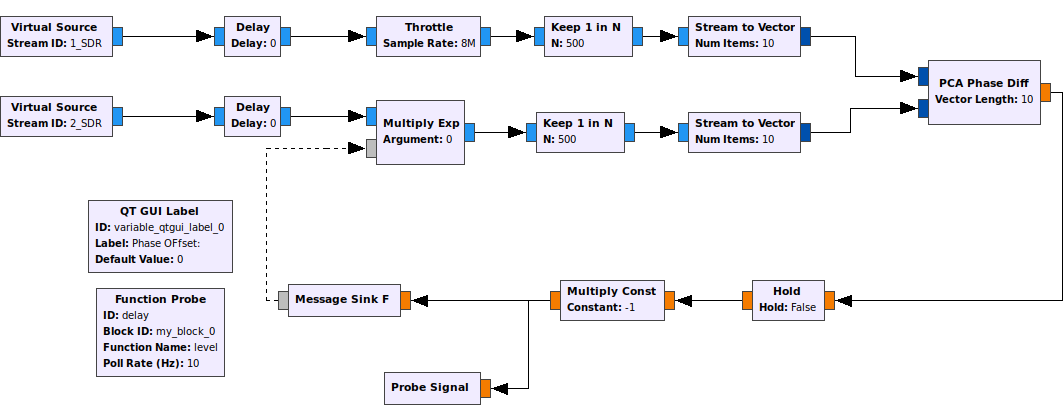
\includegraphics[width=1\linewidth]{figures/phasediff.png}
	\caption{Ước lượng và phản hồi $\textrm{phase}_\textrm{offset}$}
	\label{fig:phasediff}
\end{figure}

Kết quả thực nghiệm trên hình 2.18, khi phát NBFM ở tần số 923 MHz trên 1 BladeRF, 2 BladeRF thu, tính toán $\textrm{sample}_\textrm{offset}$ và căn chỉnh pha.
\afterpage{\clearpage}
\begin{figure}[!ht]
%\hfill
\centering
\subfigure[Tín hiệu ban đầu chưa đồng bộ]{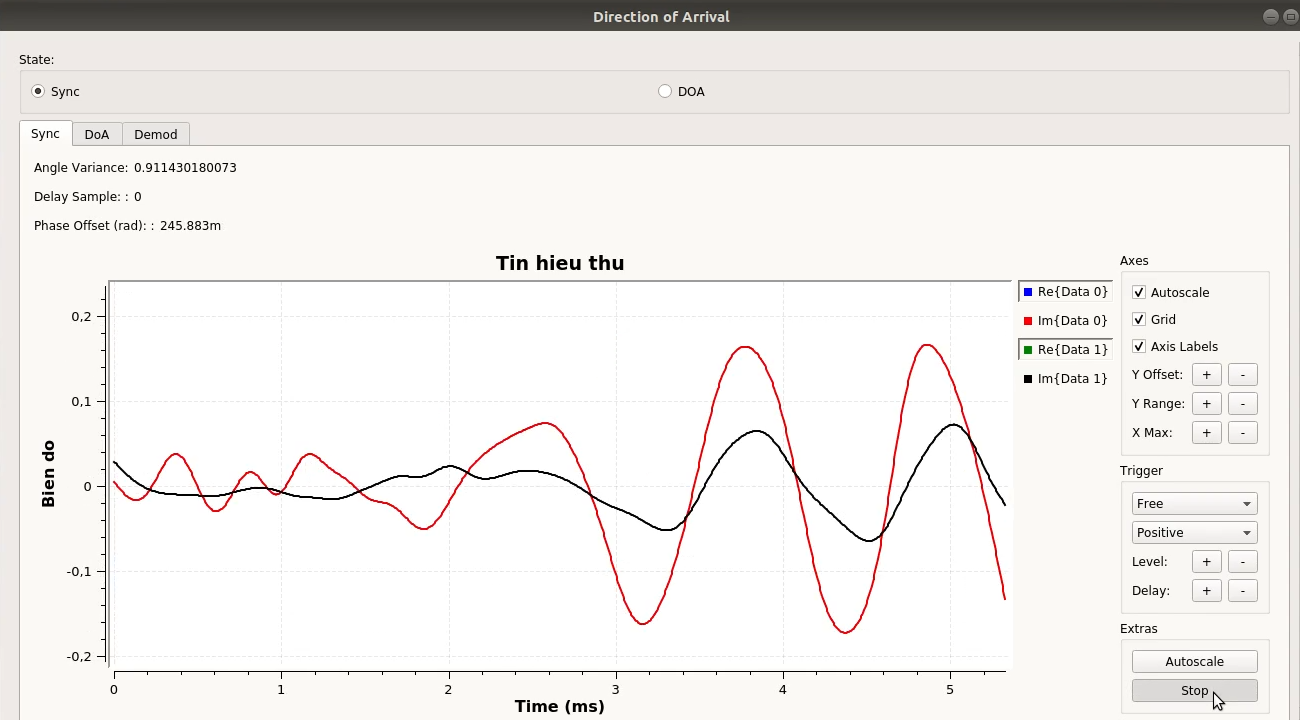
\includegraphics[width=0.8\linewidth]{figures/nonshift.png}\label{fig:nonshift}}
\hfill
\subfigure[Tín hiệu sau khi dịch mẫu và căn chỉnh pha]{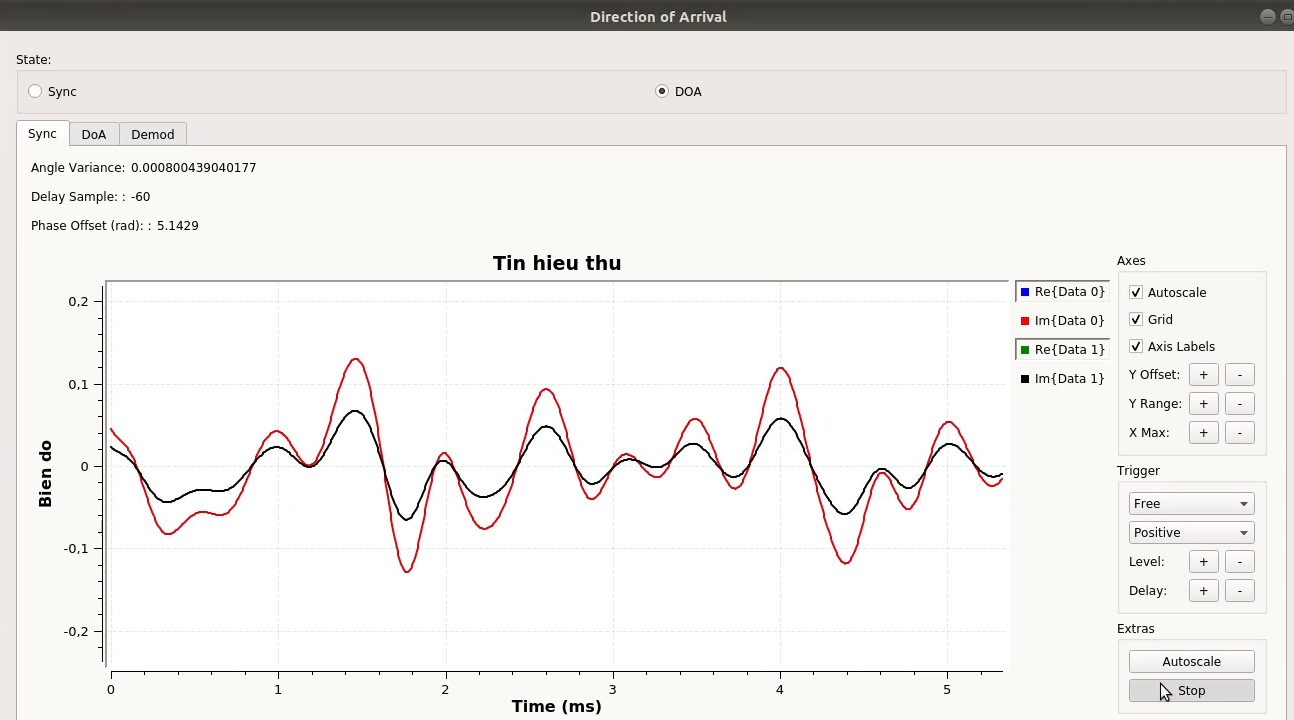
\includegraphics[width=0.8\linewidth]{figures/shifted.png}\label{fig:shifted}}
\hfill
\subfigure[Góc đầu ra ban đầu khi hệ được đồng bộ]{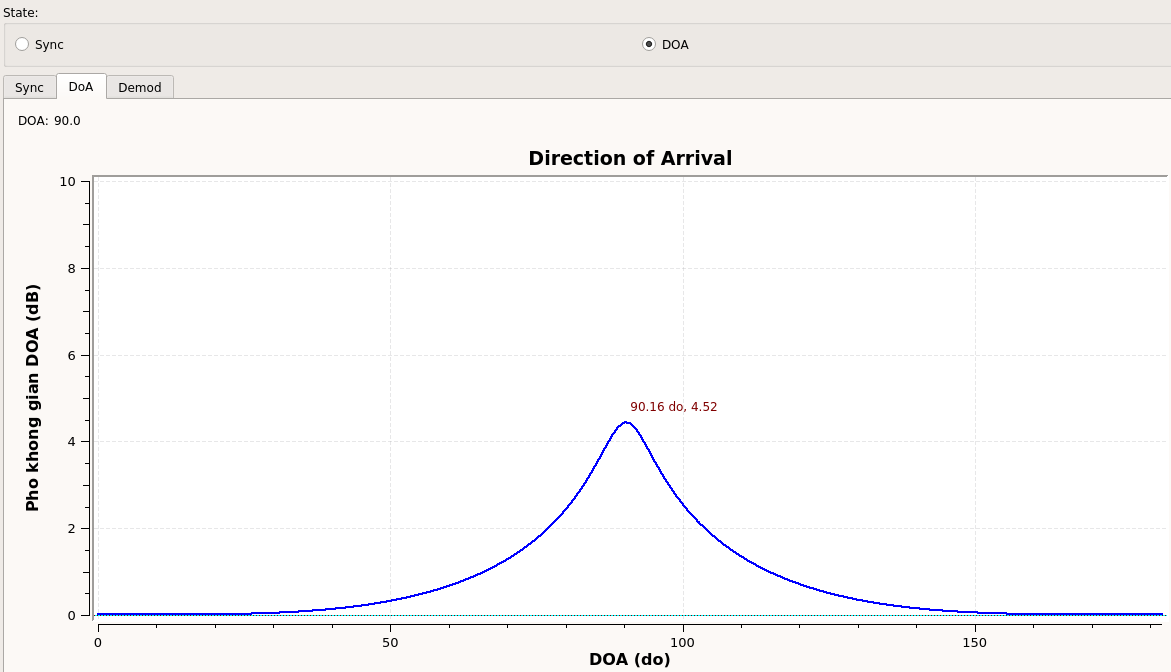
\includegraphics[width=0.8\linewidth]{figures/DOA_sync.png}
\hfill
\label{fig:DOA_sync}}
\caption{Kết quả đồng bộ hệ SDR}
\end{figure}
\newpage
\clearpage
\phantomsection

\setcounter{chapter}{2}
\chapter[{KẾT QUẢ MÔ PHỎNG, THỰC NGHIỆM HỆ THỐNG}]{Kết quả mô phỏng, thực nghiệm hệ thống}

Trong chương này, trình bày việc triển khai thuật toán MUSIC trên GNU Radio với dữ liệu: mô phỏng từ Matlab; giả lập BladeRF từ các khối trên GNU Radio; BladeRF thực. Từ đó rút ra so sánh, đánh giá kết quả thực tế so với mô phỏng.

\section{Mô phỏng hệ thống trên GNU Radio}

\subsection{Mô phỏng với dữ liệu Matlab}

Trước hết, sử dụng tín hiệu mô phỏng từ Matlab xuất ra file \textit{.mat} rồi đưa vào GNU Radio và thực hiện ước lượng hướng sóng đến từ dữ liệu, việc này đảm bảo việc lập trình khối hoạt động hiệu quả và giúp đánh giá được sai số lý tưởng của thuật toán MUSIC trước khi mô phỏng tín hiệu BladeRF. Vẫn áp dụng mô hình tín hiệu như ở mục 1.3, các thông số mô phỏng trên bảng 3.1.

\begin{table}[!h]
	\caption{Các thông số mô phỏng hệ DOA}
	\centering
	\begin{tabular}{|l|l|l|}
		\hline
		\rowcolor[HTML]{FFECEA} 
		\multicolumn{1}{|c|}{\cellcolor[HTML]{FFECEA}\textbf{Thông số}} & \multicolumn{1}{c|}{\cellcolor[HTML]{FFECEA}\textbf{Giá trị}} & \multicolumn{1}{c|}{\cellcolor[HTML]{FFECEA}\textbf{Chú thích}} \\ \hline
		$f$ & 923 Mhz & Tần số. \\ \hline
		$\lambda$ & c $\div f$ = 0,325 m & Bước sóng. \\ \hline
		M & 2 & Số phần tử anten mảng thu. \\ \hline
		d & 0,5 $\times \lambda$ & Khoảng cách giữa các phần tử anten mảng thu (ULA). \\ \hline
		D & 1 & Số phần tử nguồn. \\ \hline
		angle & 85 $\times \pi \div$ 180 & Góc tới của tín hiệu. \\ \hline
		gain & 0 & Hệ số khuếch đại. \\ \hline
		SNR & 70 dB & Tỷ lệ tín hiệu tạp âm. \\ \hline
		k & 2 $\times \pi \div \lambda$ & Hệ số sóng. \\ \hline
		K & 1024 & Số mẫu thu thập. \\ \hline
	\end{tabular}
\label{parass}
\end{table}
\begin{subequations}
\label{eq:all}
\begin{align}
\label{eq:model_a}
    \mathbf{s} &=
    \begin{bmatrix}
   	20^{\frac{SNR}{10}}\times \mathrm{randn}(1, K) + j \times \mathrm{randn}(1, K)
    \end{bmatrix}\\
\label{eq:model_b}
    \mathbf{A} &=
    \begin{bmatrix}
	10^{\frac{gain}{10}} \times \mathrm{exp}\{j \times k \times (0:M-1) \times d \times \cos(angle)\}
    \end{bmatrix}^T \\
\label{eq:model_c}
 \mathbf{n} &=
    \begin{bmatrix}
	\mathrm{randn}(M, K) + j \times \mathrm{randn}(M, K)
    \end{bmatrix} \\
\label{eq:model_d}
 \mathbf{x} &=
    \begin{bmatrix}
	\mathbf{A}\mathbf{s} + \mathbf{n}
    \end{bmatrix}
\end{align}
\end{subequations}

Sử dụng Matlab tạo mô phỏng dữ liệu đầu vào với những thông số như trên, thu được được ma trận $\mathbf{x}(t) \in \mathbb{C}^{2 \times 5000}$, lưu trữ vào file \textit{source.mat} bằng hàm có sẵn của Matlab. Việc tiếp theo là đưa dữ liệu mô phỏng vào GNU Radio thông qua việc tạo một khối nguồn cho file \textit{source.mat}. Đối với mục đích này, Synchronous Blocks được sử dụng: một khối loại bỏ đầu vào và thay thế bằng file dữ liệu mô phỏng từ Matlab tạo thành khối nguồn; một khối loại bỏ đầu ra tạo thành khối đích để tính toán và hiển thị giao diện DOA. Sử dụng Pỵthon để tiết kiệm thời gian viết khối, sơ đồ khối của việc mô phỏng thực hiện như hình \ref{fig:simulation}.
\begin{figure} [h]
	\centering
	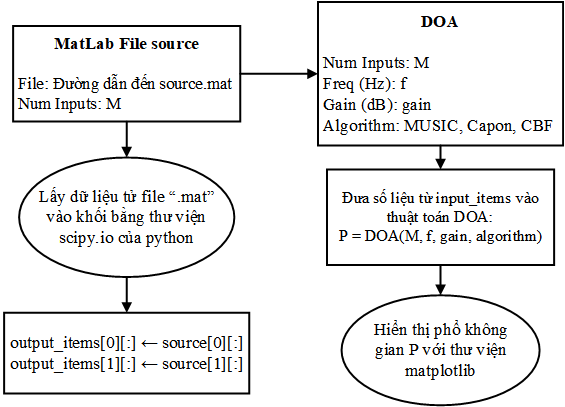
\includegraphics[width=0.8\linewidth]{figures/simulation.png}
	\caption{Sơ đồ làm việc DOA với dữ liệu mô phỏng Matlab}
	\label{fig:simulation}
\end{figure}

Liên kết hai khối với nhau và nhập các thông số đầu vào của hệ và chạy hệ thống. Kết quả trên GNU Radio Companion thu được như phụ lục hình \ref{fig:simulation1}. Tiến hành thay đổi góc đầu vào từ file dữ liệu Matlab và chạy hệ thống nhiều lần, mỗi lần sẽ thu được kết quả như hình \ref{fig:simulation2}.
\begin{figure}[!h]
%\hfill
\subfigure[Kết quả của GNU Radio]{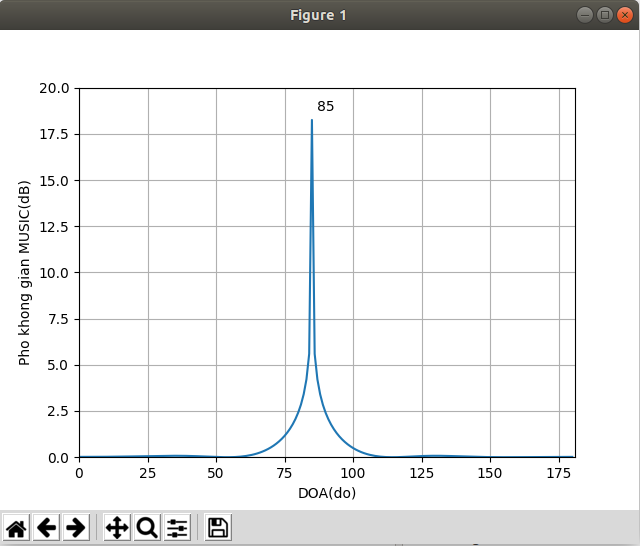
\includegraphics[width=0.49\linewidth]{figures/simulation3.png}}
\hfill
\subfigure[Kết quả của Matlab]{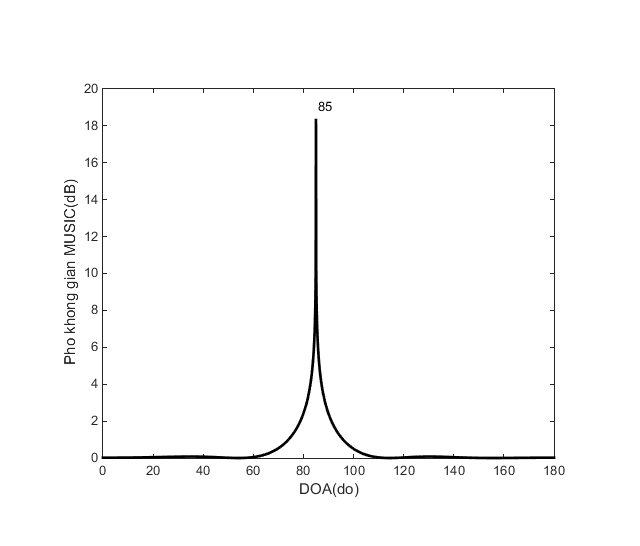
\includegraphics[width=0.49\linewidth]{figures/simulation4.png}}
\hfill
\caption{Kết quả ước lượng DOA với dữ liệu mô phỏng Matlab}
\label{fig:simulation2}
\end{figure}

Do dữ liệu mô phỏng là hoàn toàn khớp với các điều kiện lý tưởng, sai số của thuật toán MUSIC trên GNU Radio giống như trên lý thuyết \cite{Transactions1989, Quynh2015}, sử dụng thông số CRB (Cramér–Rao bound) cho một nguồn để đánh giá sai số ước lượng:
\begin{equation}
	\mathrm{CRB}(\phi) = \mathbf{J}^{-1} 
\end{equation}
với $\mathbf{J}^{-1}$ là ma trận Fisher, được biểu diễn ở phương trình (3.2):
\begin{equation}
\begin{split}
\mathbf{J} &= K \cdot \mathrm{trace} \left \{ \mathbf{R}_\mathbf{x}^{-1} \frac{\partial \mathbf{R}_\mathbf{x}}{\partial \phi} \mathbf{R}_\mathbf{x}^{-1} \frac{\partial \mathbf{R}_\mathbf{x}}{\partial \phi} \right \} \\
&= \frac{2 \mathrm{SNR}^2}{(1 + \mathrm{SNR} |\mathbf{a}|^2)^2} [2(\Re  (\mathbf{a}^{H} \dot{\mathbf{a}}))^2 + (1 + \mathrm{SNR} |\mathbf{a}|^2)(|\mathbf{a}|^2 |\dot{\mathbf{a}}|^2 - |\mathbf{a}^H \dot{\mathbf{a}}|^2)]
\end{split} 
\end{equation}
với $\dot{\mathbf{a}}_\phi = \partial\mathbf{a}/\partial\phi$. Hình \ref{fig:RMSE} biểu diễn CRB của mảng ULA với các tham số: $M$ = 2, SNR = 70 dB, số mẫu $K$ = 1024. Như vậy, thấy rằng mảng ULA có lỗi ước lượng nhỏ với các góc ở trục vuông và sai số lớn với các góc ở trục dọc so với mảng anten thu.
\begin{figure} [!h]
	\centering
	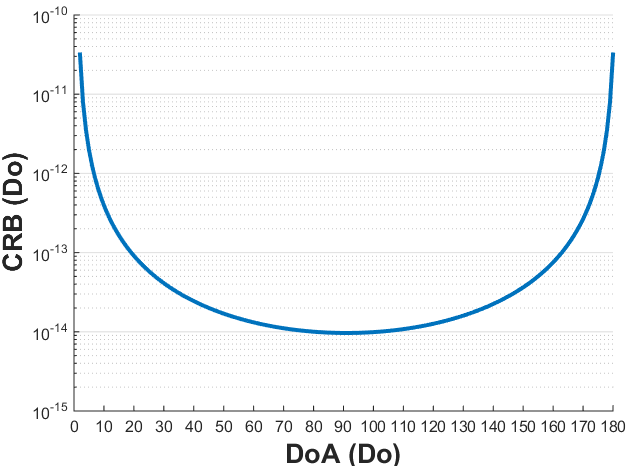
\includegraphics[width=0.64\linewidth]{figures/CRB.png}
	\caption{CRB của mảng anten ULA}
	\label{fig:RMSE}
\end{figure}

\subsection{Mô phỏng với dữ liệu giả lập BladeRF}

Sau khi đã mô phỏng thành công với dữ liệu từ Matlab, tiếp tục mô phỏng dữ liệu BladeRF thực với tín hiệu đầu vào là âm thanh được điều chế NBFM (chi tiết tham số điều chế, phổ, SNR được trình bày ở mục 3.2.1). Vẫn sử dụng thông số mô phỏng như bảng 3.1, sau khi được mã hóa, chia tín hiệu thành 2 luồng đi qua kênh truyền với các thông số như bảng \ref{tab:simu}, các khối mô phỏng tương ứng trên GNU Radio được biểu diễn ở phụ lục hình \ref{fig:bladesimu}.
\begin{table}[!h]
\centering
\caption{Các thông số mô phỏng tín hiệu BladeRF qua kênh truyền}
\arrayrulecolor{black}
\begin{tabular}{|l|l|l|} 
	\hline
	\rowcolor[rgb]{1,0.91,0.906} \multicolumn{1}{|c|}{ \textbf{Mô phỏng} } & \multicolumn{1}{c|}{\textbf{Thông số mô phỏng} } & \multicolumn{1}{c|}{\textbf{Giá trị} }  \\ 
	\hline
	{\cellcolor[rgb]{0.937,0.937,0.937}}                                   & Giá trị tạp âm                                   & 0,01 (1\% biên độ tối đa của tín hiệu)  \\ 
	\hhline{|>{\arrayrulecolor[rgb]{0.937,0.937,0.937}}->{\arrayrulecolor{black}}--|}
	{\cellcolor[rgb]{0.937,0.937,0.937}}                                   & Gieo hạt của tạm âm                              & 1000                                    \\ 
	\hhline{|>{\arrayrulecolor[rgb]{0.937,0.937,0.937}}->{\arrayrulecolor{black}}--|}
	{\cellcolor[rgb]{0.937,0.937,0.937}}                                   & Số tín hiệu đa đường                             & 8                                       \\ 
	\hhline{|>{\arrayrulecolor[rgb]{0.937,0.937,0.937}}->{\arrayrulecolor{black}}--|}
	{\cellcolor[rgb]{0.937,0.937,0.937}}                                   & Phân bố nhiễu đa đường                           & Rayleigh                                \\ 
	\hhline{|>{\arrayrulecolor[rgb]{0.937,0.937,0.937}}->{\arrayrulecolor{black}}--|}
	\multirow{-5}{*}{{\cellcolor[rgb]{0.937,0.937,0.937}}Kênh truyền}      & Gieo hạt nhiễu đa đường                          & 1000                                    \\ 
	\hline
	{\cellcolor[rgb]{1,0.988,0.62}}                                        & Trễ mẫu                                          & 1000 (mẫu)                              \\ 
	\hhline{|>{\arrayrulecolor[rgb]{1,0.988,0.62}}->{\arrayrulecolor{black}}--|}
	\multirow{-2}{*}{{\cellcolor[rgb]{1,0.988,0.62}}Phần cứng BladeRF}     & Độ lệch pha ban đầu                              & 45$^{\circ}$ = 0,78539 (rad)            \\
	\hline
\end{tabular}
\label{tab:simu}
\end{table}

Chạy mô phỏng với các tệp âm thanh khác nhau, mỗi tệp chạy 5 lần và ghi lại kết quả thông số đồng bộ và vector giá trị riêng từ hệ DOA, sau đó tính trung bình và đưa vào bảng \ref{tab:kqsync}.

\begin{table}[!h]
\centering
\caption{Kết quả mô phỏng đồng bộ}
\begin{tabular}{|l|c|c|cc|} 
	\hline
	\rowcolor[rgb]{1,0.91,0.906} \multicolumn{1}{|c|}{ \textbf{Nguồn tín hiệu} }                   & \textbf{Độ trễ (mẫu)}  & \textbf{Độ lệch pha (rad)}  & \multicolumn{2}{c|}{\textbf{Vector giá trị riêng} }  \\ 
	\hline
	\multirow{2}{*}{Tệp âm thanh 1}                                                                & \multirow{2}{*}{994,6}   & \multirow{2}{*}{0,72986}    & 0,00048259 & 0                                       \\
	&                        &                             & 0          & 0,04719653                              \\ 
	\hline
	\multirow{2}{*}{Tệp âm thanh 2 }                                                               & \multirow{2}{*}{991,25}  & \multirow{2}{*}{0,72999}    & 2,03512e-5 & 0                                       \\
	&                        &                             & 0          & 0,0863451                               \\ 
	\hline
	\multirow{2}{*}{\begin{tabular}[c]{@{}l@{}}Tệp âm thanh 1 bỏ\\qua trễ phần cứng \end{tabular}} & \multirow{2}{*}{}      & \multirow{2}{*}{}           & 1,241364-5 & 0                                       \\
	&                        &                             & 0          & 0,0034562                               \\
	\hline
\end{tabular}
\label{tab:kqsync}
\end{table}

Từ bảng \ref{tab:kqsync}, nhận thấy việc ước lượng độ trễ bằng tương quan chéo của tín hiệu NBFM cho kết quả chưa hoàn toàn chính xác (< 10 mẫu), kéo theo đó sẽ là sai số khi ước lượng độ lệch pha ở mức 0,056 (rad). Thông số đánh giá còn lại là ma trận vector giá trị riêng, biểu hiện sự phân biệt giữa tín hiệu và tạp âm, với tỷ lệ trung bình $10^2$ đến $10^3$, tín hiệu NBFM đủ để xuất hiện đỉnh phổ trên phổ không gian MUSIC.

Từ kết quả mô phỏng đồng bộ chưa hoàn toàn chính xác khi sử dụng NBFM, cần phải mô phỏng ước lượng hướng sóng đến dựa trên những kết quả đồng bộ phía trên để có đánh giá chính xác nhất. Kết quả sẽ được tính lỗi căn trung bình bình phương RMSE của góc thu được ($\phi$) so với góc mô phỏng ($\bar{\phi}$) như trên công thức (3.3) với D là số lần thu thập kết quả, sai số được biểu diễn trên hình \ref{fig:kqnbfm}.
\begin{equation}
	\mathrm{RMSE} = \sqrt{\frac{1}{D}\sum_{i=1}^{D}(\phi_i - \bar{\phi}_i)} 
\end{equation}

\begin{figure} [!ht]
	\centering
	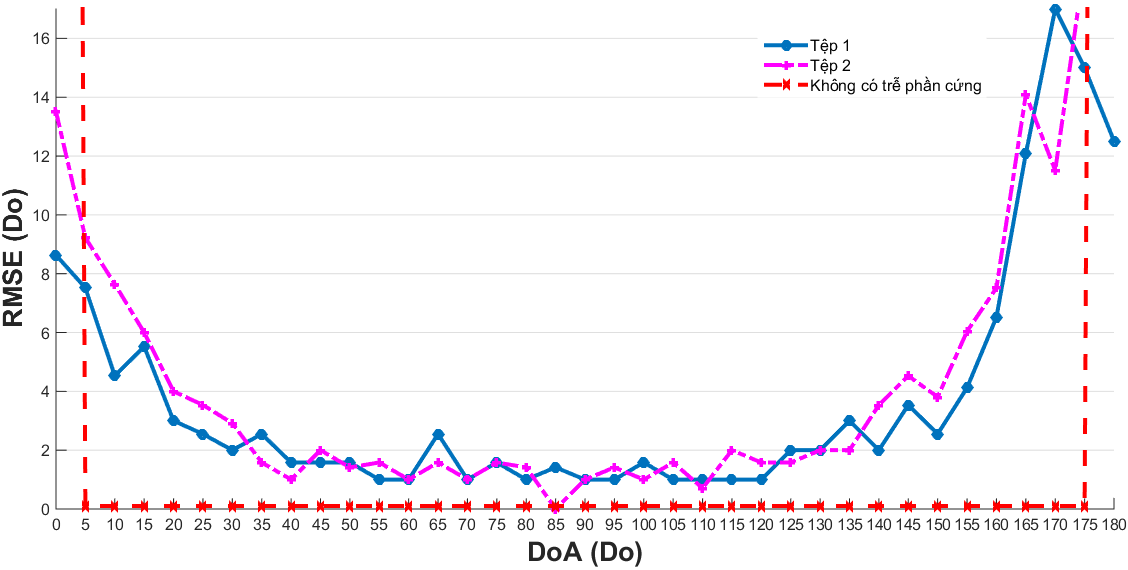
\includegraphics[width=1\linewidth]{figures/kqnbfm.png}
	\caption{RMSE: Mô phỏng dữ liệu BladeRF qua kênh truyền}
	\label{fig:kqnbfm}
\end{figure}

Như vậy so với CRB hay mô phỏng hệ thống không chịu ảnh hưởng bởi trễ phần cứng gây ra bởi BladeRF thì dạng đồ thị của RMSE khi sử dụng NBFM làm tín hiệu nguồn phát vẫn giữ được đúng hình dạng là sai số nhỏ ở những góc gần 90$^{\circ}$ và tăng dần ở hai biên phổ không gian. Tuy nhiên với các tệp âm thanh nguồn khác nhau, việc đồng bộ hệ BladeRF sẽ cho kết quả khác nhau và dẫn đến sai số góc ước lượng cũng là khác nhau nhưng không quá nhiều.

Kết luận lại, dù vẫn còn sai số trong việc đồng bộ hệ BladeRF tuy nhiên sai số vẫn đủ nhỏ để tiếp tục sử dụng tín hiệu NBFM thực hiện hệ DOA trên hệ thống BladeRF thực.

\section{Thực nghiệm hệ thống}

Với tiền đề là việc mô phỏng thành công  được dữ liệu BladeRF trên GNU Radio, tiếp theo là thực nghiệm hệ thống DOA trên hệ BladeRF thực, trong phần này sẽ trình bày điều kiện và kết quả thực nghiệm, cuối cùng đưa ra nhận xét từ kết quả thu được.

\subsection{Tín hiệu nguồn phát và thiết lập hệ thu}

Dữ liệu thực tế được dùng cho hệ tìm hướng sóng đến rất da dạng như: tín hiệu FM của các đài phát thanh, tín hiệu chuẩn DVB-T của đài truyền hình, GSM hay WiFi,... Trong khóa luận này, tín hiệu NBFM được lựa chọn để làm tín hiệu nguồn phát, vừa để đồng bộ hệ SDR thu, vừa để làm tín hiệu nguồn cho việc xác định hướng sóng đến. Lý do lựa chọn NBFM, vì đây là điều chế tín hiệu băng hẹp phù hợp với mô hình tín hiệu ban đầu của thuật toán.

NBFM: Điều chế NBFM trên GNU Radio với file nguồn là file âm thanh nén ở chuẩn WAV (Waveform Audio File Format). Flow-graph phụ lục hình \ref{fig:NBFM} là sơ đồ điều chế tiêu chuẩn NBFM cho tệp âm thanh WAV, với tín hiệu đầu ra băng hẹp 5,3 kHz (có phổ như hình \ref{fig:nbfmspectrum}, SNR trên 70 dB) và chỉ cần một bộ lọc thông thấp 5 kHz và khối giải điều chế NBFM tiêu chuẩn là đủ để giải điều chế.
\begin{figure} [!h]
	\centering
	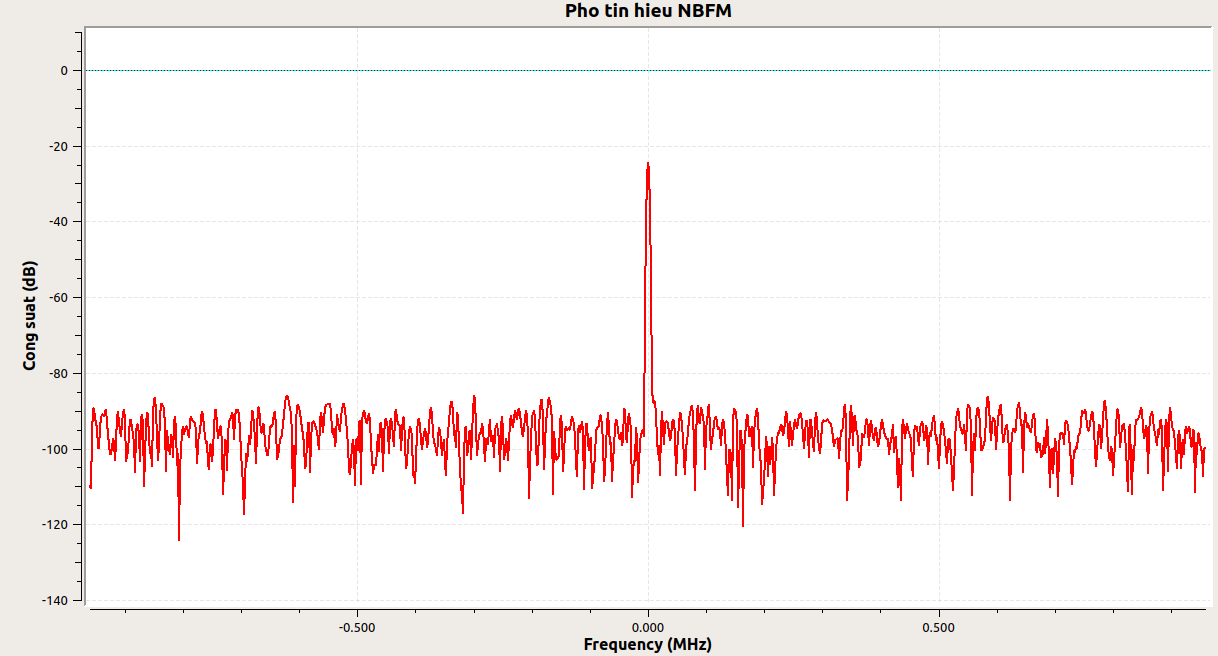
\includegraphics[width=1\linewidth]{figures/nbfmspectrum.png}
	\caption{Phổ của tín hiệu tín hiệu NBFM}
	\label{fig:nbfmspectrum}
\end{figure}

Đối với hệ thu, các bước đồng bộ và ước lượng DOA trình bày ở Chương 2 được kết hợp với nhau trên GNU Radio. Trước hết thực hiện các thiết lập trên \textit{bladeRF-cli} như chia sẻ xung đồng hồ qua cổng SMB, hiệu chỉnh CFO của BladeRF. Sau đó sử dụng flow-graph trên phụ lục hình \ref{fig:DoA_FM} phía dưới để đồng bộ và ước lượng DOA. 
%\newpage

\subsection{Tình huống thực nghiệm}

Bố trí hệ thu phát sử dụng BladeRF để triển khai việc ước lượng hướng sóng đến, trên hình \ref{fig:realsys} là hệ thống được cài đặt hoàn chỉnh, gồm 1 BladeRF phát và 2 BladeRF thu, cả 3 anten được sử dụng đều là anten không định hướng VERT2450. Cấu hình phần cứng và phần mềm của 2 máy tính thực hiện việc phát và thu trong khóa luận được nêu ra trong bảng \ref{table:hw}. Tần số được chọn là 923 MHz, là tần số nằm trong khoảng giữa của đường lên và xuống trong GSM900.
\begin{figure} [!h]
	\centering
	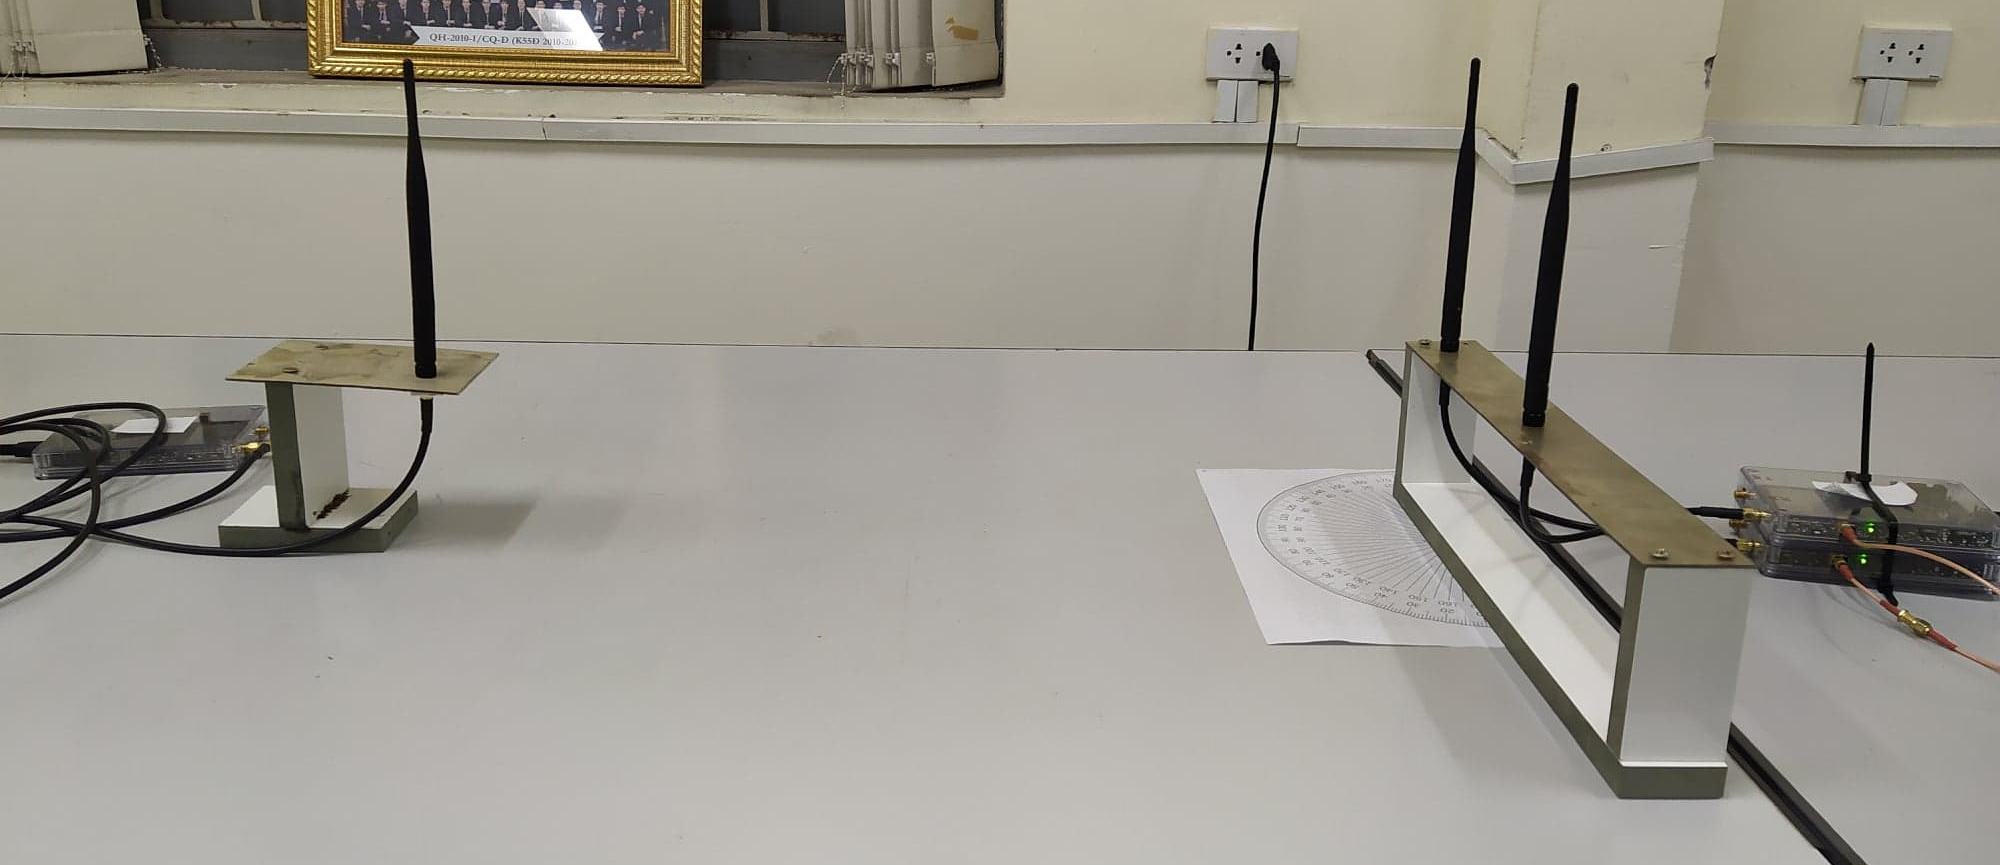
\includegraphics[width=1\linewidth]{figures/realsys.jpg}
	\caption{Sơ đồ bố trí hệ DOA thực}
	\label{fig:realsys}
\end{figure}
\begin{table}[!h]
\centering
\caption{Thông số máy tính}
\begin{tabular}{|l|c|c|} 
	\hline
	\rowcolor[rgb]{1,0.91,0.906} \multicolumn{1}{|c|}{ \textbf{Thông số} } & \textbf{Bên phát}    & \textbf{Bên thu}     \\ 
	\hline
	CPU                                                                    & Intel Core I5-4800MQ & Intel Core I5-4210M  \\ 
	\hline
	RAM                                                                    & 8 GB                 & 8 GB                 \\ 
	\hline
	Hệ điều hành                                                           & Ubuntu 16.04 LTS     & Ubuntu 18.04 LTS     \\ 
	\hline
	Phiên bản GNU Radio                                                    & 3.7.11               & 3.7.11               \\
	\hline
\end{tabular}
\label{table:hw}
\end{table}

Điều kiện thực nghiệm là phòng 204, nhà G2, Đại học Công Nghệ - Đại học Quốc Gia Hà Nội, tiến hành thực nghiệm 350 lần, xác định hướng sóng đến từ các góc khác nhau, để giảm thiểu sai số chủ quan độ phân giải khi thực nghiệm ở mức 5$^{\circ}$, bố trí hệ thống ở 3 vị trí khác nhau để đưa ra ảnh hưởng của môi trường đến độ chính xác của hệ DOA.
\newpage
\subsection{Kết quả thực nghiệm}

\begin{itemize}
	\item[$\ast$] \textbf{Phổ không gian}
\end{itemize} 

Hình \ref{fig:kqsync} biểu diễn kết phổ không gian của thuật toán MUSIC trên GNU Radio trong trường hợp: có tín hiệu đến ở góc 90$^{\circ}$, không có tín hiệu nào đến và tín hiệu mô phỏng từ Matlab.

\begin{figure} [!h]
	\centering
	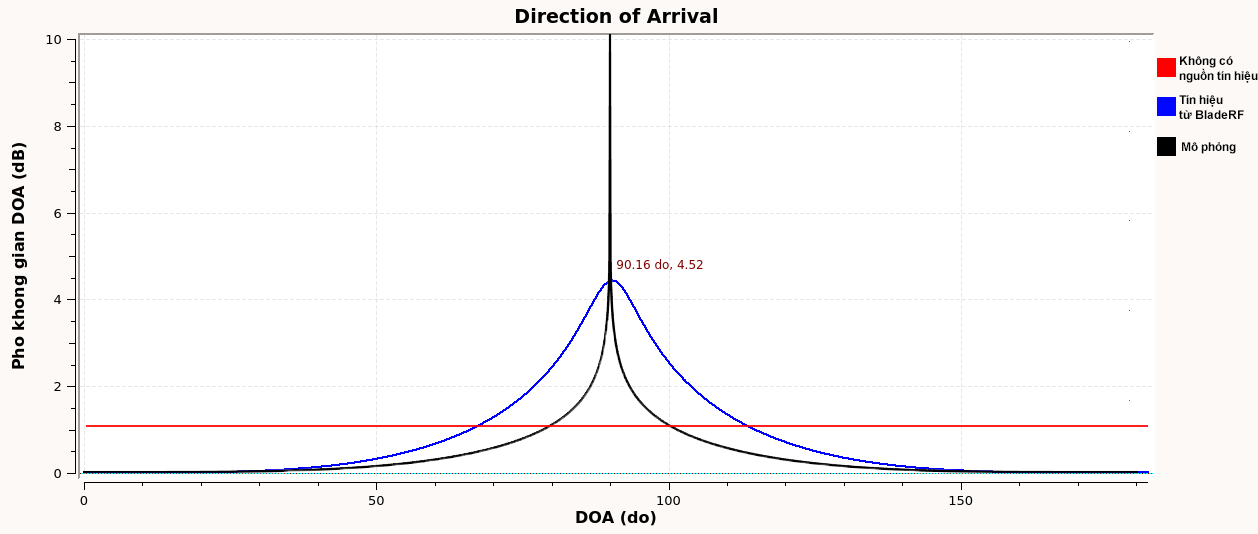
\includegraphics[width=1\linewidth]{figures/kqsync.png}
	\caption{So sánh phổ không gian trên thực tế và mô phỏng}
	\label{fig:kqsync}
\end{figure}

Hình dạng phổ không gian khi thực nghiệm là giống với kết quả khi mô phỏng, tuy nhiên về đỉnh phổ thì lại thấp hơn so với mô phỏng và độ rộng của đỉnh phổ cũng lớn hơn mô phỏng, điều này xảy ra do tín hiệu thực có biên độ chênh lệch với nhau lớn, đây là vấn đề do phần cứng, hệ số khuếch đại, việc khắc phục sẽ được thực hiện trong tương lai. Còn khi không có tín hiệu đến, phổ DOA đã cho kết quả đúng khi không xuất hiện đỉnh phổ nào.

\begin{itemize}
	\item[$\ast$] \textbf{Kết quả đồng bộ}
\end{itemize} 

Kết quả mô phỏng khi hệ thống DOA đồng bộ và không đồng bộ như hình \ref{fig:simukq}, kết cho cho thấy sau khi được đồng bộ về lượng mẫu trễ và pha sai lệch giữa các tín hiệu từ BladeRF, kết quả phổ DOA thu được sẽ giữ ở một đỉnh phổ ổn định và chính xác, còn khi hệ BladeRF chưa đồng bộ đỉnh phổ liên tục nhảy giữa các vị trí khác nhau, không thể xác định hướng sóng đến.

\begin{figure} [!h]
	\centering
	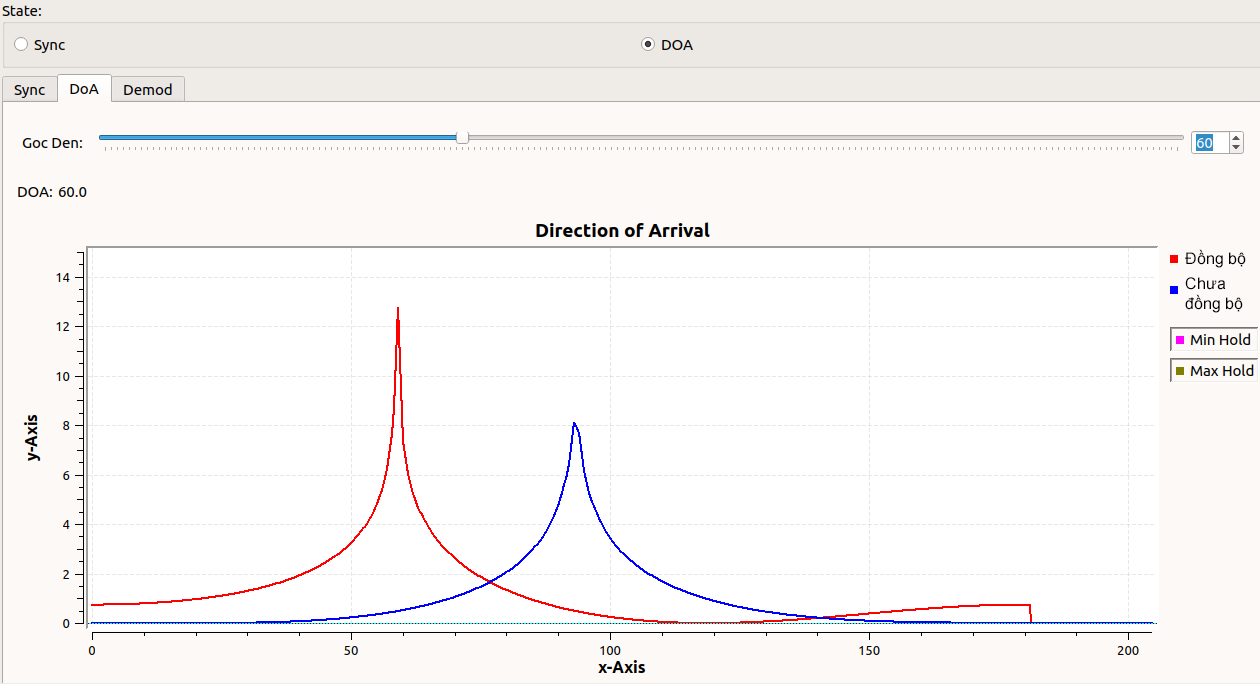
\includegraphics[width=1\linewidth]{figures/simukq.png}
	\caption{Kết quả DOA mô phỏng khi hệ SDR đồng bộ}
	\label{fig:simukq}
\end{figure}
\newpage
Qua kiểm nghiệm thực tế, kết quả cũng thu được như trên mô phỏng tuy nhiên độ rộng của đỉnh phổ thì lớn hơn mô phỏng nhưng kết quả ước lượng vẫn chính xác khi hệ BladeRF được đồng bộ. Đối với hệ BladeRF chưa được đồng bộ, góc ước lượng được luôn thay đổi và không thể xác định hướng sóng đến.

\begin{figure} [!h]
	\centering
	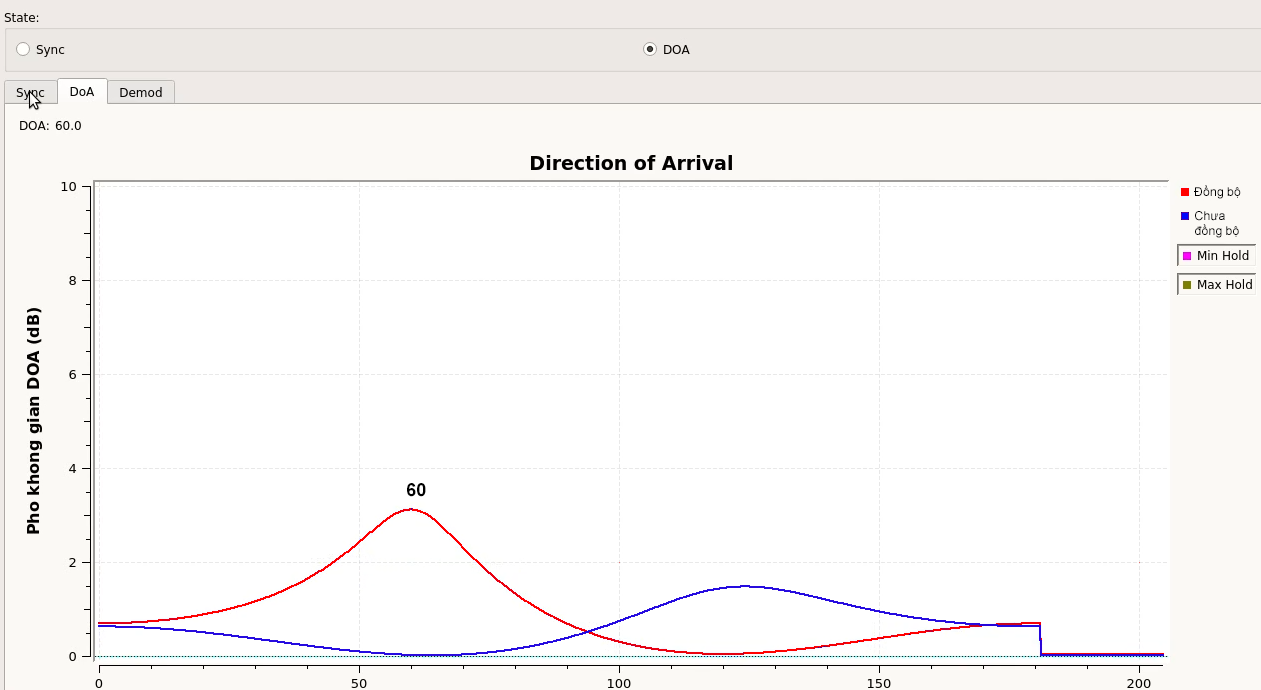
\includegraphics[width=1\linewidth]{figures/kqreal.png}
	\caption{Kết quả DOA thực nghiệm khi hệ SDR đồng bộ}
	\label{fig:kqreal}
\end{figure}
\newpage
\begin{itemize}
	\item[$\ast$] \textbf{Khảo sát lỗi ước lượng của hệ thống}
\end{itemize} 

\textbf{- Kết quả ước lượng theo độ $\phi = 0 \rightarrow 180$}

Hình \ref{fig:kq1} là RMSE của quá trình thực nghiệm ước lượng DOA trên BladeRF thực so với kết quả mô phỏng dữ liệu BladeRF. Nhận thấy, dạng biểu đồ RMSE thu được từ thực nghiệm là tương đồng với mô phỏng và CRB được ước lượng ở hình \ref{fig:RMSE}, sai số ở các góc gần 90$^{\circ}$ nhỏ, và tăng dần ở các góc ở hai biên của phổ không gian.

Ở khoảng góc từ 60$^{\circ}$ đến 135$^{\circ}$, sai số dưới 6$^{\circ}$, và do chỉ sử dụng 2 phần tử anten mảng thu nên mức sai số này là chấp nhận được.
\begin{figure} [!h]
	\centering
	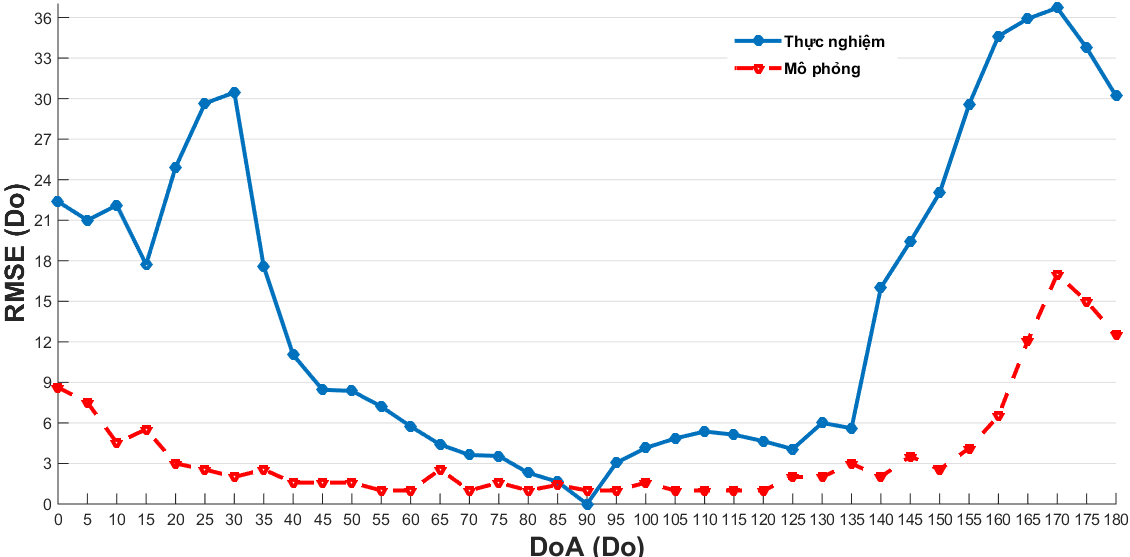
\includegraphics[width=1\linewidth]{figures/kq1.png}
	\caption{RMSE: DOA thực nghiệm và mô phỏng}
	\label{fig:kq1}
\end{figure}

\textbf{- Kết quả ước lượng theo vị trí}

Thực nghiệm thêm để xem xét vị trí đặt hệ DOA hay kênh truyền có ảnh hưởng đến kết quả ước lượng hướng sóng đến hay không, đặt hệ ở 3 vị trí khác nhau, kết quả RMSE thu được như hình \ref{fig:dvbt_1}.
\begin{figure} [!h]
	\centering
	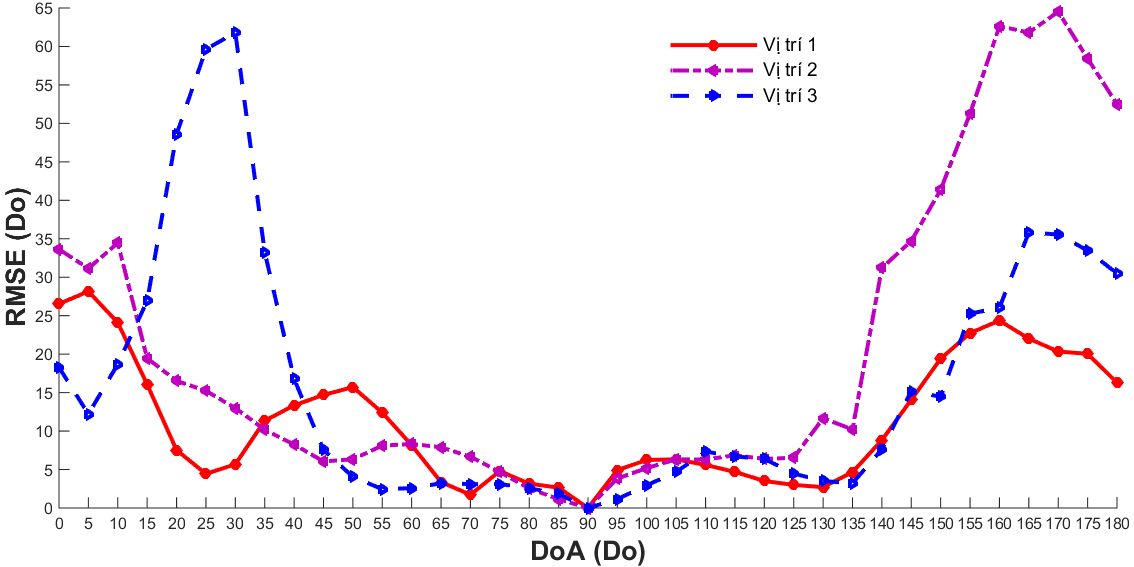
\includegraphics[width=1\linewidth]{figures/dvbt_1.png}
	\caption{RMSE: DOA ở từng vị trí thực nghiệm}
	\label{fig:dvbt_1}
\end{figure}

Từ kết quả RMSE thu được, có thể nhận thấy khoảng góc từ 60$^{\circ}$ đến 135$^{\circ}$ vẫn cho sai số thấp tương đương nhau ở cả 3 vị trí. Ở các góc ngoài khoảng trên, kết quả rất dễ bị ảnh hưởng bởi nhiễu đa đường, gây ra sai số nhảy vọt ở một số khoảng góc có nhiều vật cản.

Kết luận hệ ước lượng hướng sóng đến, vẫn hoạt động ở các điều kiện kênh truyền khác nhau.

\textbf{- Kết quả ước lượng với dữ liệu khác nhau}

Tuy theo lý thuyết, thuật toán MUSIC áp dụng cho mô hình tín hiệu băng hẹp, nhưng trong khóa luận này, sẽ mở rộng thêm và sử dụng tín hiệu băng rộng cho hệ DOA sử dụng thuật toán MUSIC.

Tín hiệu băng rộng được sử dụng là DVB-T, tín hiệu chuẩn thu truyền hình số mặt đất tiêu chuẩn ở Việt Nam. Việc điều chế, thông số, phổ DVB-T trên GNU Radio như sau: 

DVB-T: Điều chế chuẩn DVB-T trên GNU Radio với file nguồn là file video nén ở chuẩn TS (Transport Stream). Flow-graph ở phụ lục hình \ref{fig:dvbt} truyền video ở băng thông 8 MHz, chòm sao QPSK, tốc độ mã 7/8, khoảng bảo vệ 1/32, tốc độ lấy mẫu 10 MHz, tần số 923 MHz. Chi tiết hơn về việc sử dụng BladeRF truyền nhận DVB-T có tại \cite{BogdanDIA2015}.

Phổ tín hiệu DVB-T được truyền, và thu lại như hình \ref{fig:spectrum}, nhận thấy do sử dụng OFDM nên phổ của DVB-T bị trải đều trên dải tần số, dẫn đến SNR ở mức 37,5 dB so với trên 70 dB của NBFM.

\begin{figure} [!h]
	\centering
	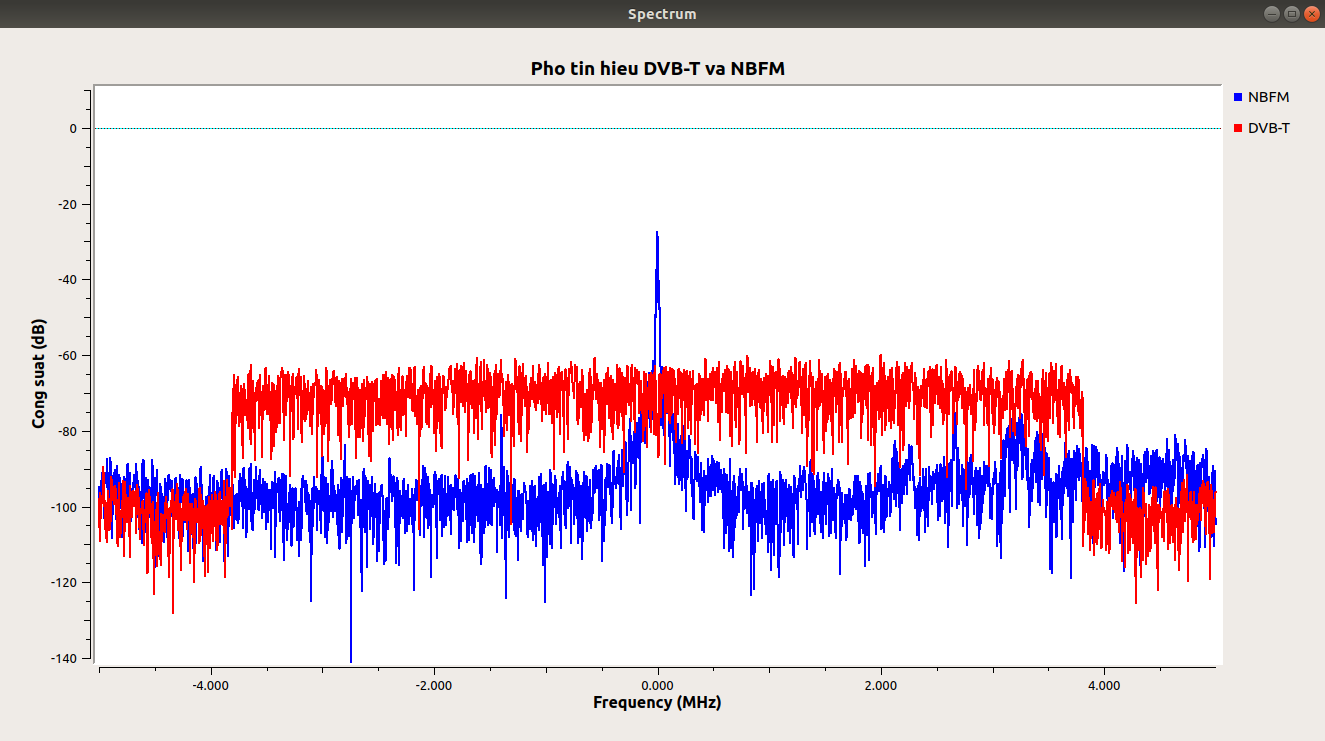
\includegraphics[width=1\linewidth]{figures/spectrum2.png}
	\caption{Phổ tín hiệu DVB-T và NBFM thu được}
	\label{fig:spectrum}
\end{figure}

Qua mô phỏng BladeRF trên GNU Radio, kết quả đồng bộ từ tín hiệu DVB-T thu được như bảng \ref{tab:kqdvbt}. Với tính tương quan thấp hơn của NBFM, kết quả ước lượng sai số phần cứng BladeRF từ tín hiệu DVB-T là hoàn toàn khớp với các thông số mô phỏng.
\begin{table}[!h]
	\caption{Kết quả mô phỏng đồng bộ bằng tín hiệu DVB-T}
	\centering
	\begin{tabular}{|l|l|l|cc|} 
		\hline
		\rowcolor[rgb]{1,0.91,0.906} \multicolumn{1}{|c|}{ \textbf{Loại tín hiệu} } & \multicolumn{1}{c|}{\textbf{Độ trễ (mẫu)} } & \multicolumn{1}{c|}{\textbf{Độ lệch pha (rad)} } & \multicolumn{2}{c|}{\textbf{Vector giá trị riêng} }  \\ 
		\hline
		\multirow{2}{*}{DVB-T}                                                      & \multirow{2}{*}{1000}                       & \multirow{2}{*}{0,78539}                         & 1,4544877e-11 & 0                                    \\
		&                                             &                                                  & 0             & 9,0942479e-04                        \\
		\hline
	\end{tabular}
\label{tab:kqdvbt}
\end{table}

Tuy nhiên qua thực nghiệm sử dụng tín hiệu băng rộng DVB-T cho đồng bộ và xác định hướng sóng đến, nhận thấy nếu thu toàn bộ 8 MHz băng thông của DVB-T sử dụng cho đồng bộ hệ BladeRF thì không thể thu được kết quả như mô phỏng. Vì vậy thay vì sử dụng toàn bộ dải băng rộng của tín hiệu DVB-T, tác giả khóa luận chỉ thu một phần của phổ DVB-T là 2 MHz, sau đó sử dụng thêm bộ lọc thông thấp 5 kHz như NBFM để lấy một phần nhỏ của tín hiệu DVB-T ban đầu, điều này khiến việc giải điều chế tín hiệu đồng thời như NBFM là không thể, tuy nhiên lại cho kết quả tốt khi xác định hướng sóng đến.

%Quay ngược lại mô phỏng việc sử dụng băng thông bộ thu chỉ 2 MHz và bộ lọc 5 kHz cho tín hiệu DVB-T, kết quả đồng bộ vẫn khớp với các thông số ban đầu đưa vào.
\newpage
Kết quả thực nghiệm trên hình \ref{fig:dvbt_3} khi thực nghiệm DOA tại một vị trí chỉ thay đổi tín hiệu bên phát, cho thấy dù ở khoảng 135$^{\circ}$ đến 180$^{\circ}$ sai số của DVB-T là nhỏ hơn NBFM nhưng nhìn chung thì trong khoảng góc quan trọng nhất là xung quanh 90$^{\circ}$ và hình dạng của đồ thị sai số của hai loại tín hiệu này vẫn là giống nhau và giữ được hình dạng như CRB.
\begin{figure} [!h]
	\centering
	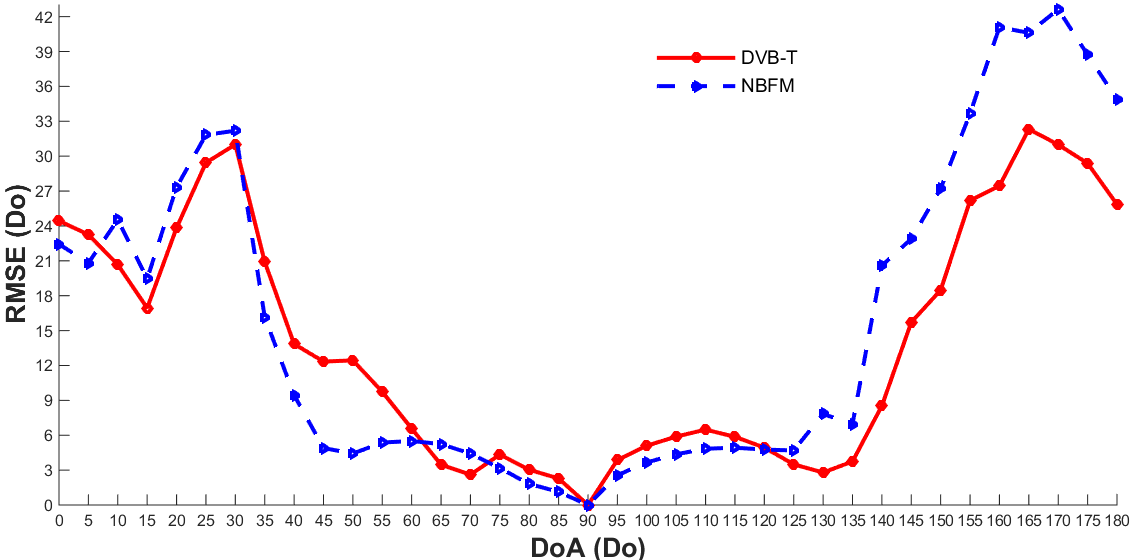
\includegraphics[width=1\linewidth]{figures/dvbt_3.png}
	\caption{RMSE: DOA với tín hiệu NBFM và DVB-T}
	\label{fig:dvbt_3}
\end{figure}

Kết luận lại, sử dụng tín hiệu băng rộng cho hệ DOA sử dụng thuật toán MUSIC hoàn toàn khả thi, kết quả thu được vẫn tốt giống như tín hiệu băng hẹp NBFM, tuy nhiên để tối ưu hơn hệ thống và tận dụng hết ưu thế của điều chế OFDM trong tín hiệu DVB-T thì tác giả cần phải tiếp tục nghiên cứu và phát triển thêm.
\newpage
\clearpage
\phantomsection

\addcontentsline{toc}{chapter}{{KẾT LUẬN VÀ HƯỚNG NGHIÊN CỨU TIẾP THEO}}

\chapter*{Kết luận và hướng nghiên cứu tiếp theo}
\section*{1. Kết luận của khóa luận tốt nghiệp}
Dựa trên các phân tích, mô phỏng, thực thi thuật toán đã triển khai ở các phần trên, chúng tôi có một số kết luận sau:

- Nếu chỉ sử dụng 2 BladeRF như trong khóa luận, việc ước lượng góc vẫn là khả thi khi ở trong khoảng từ 60$^{\circ}$ đến 135$^{\circ}$ với sai số dưới 6$^{\circ}$. Tuy nhiên để tăng độ chính xác của thuật toán, việc tăng thêm số phần tử trong mảng thu là điều bắt buộc.

- Hệ thống có thể hoạt động ở các điều kiện kênh truyền khác nhau.

- Hệ thống vẫn hoạt động chính xác với tín hiệu băng rộng và cho ra kết quả tương đồng với tín hiệu băng hẹp.

Kết quả của hệ thống vẫn còn phụ thuộc vào loại nguồn tín hiệu dùng để đồng bộ, và điều kiện kênh truyền đặc biệt là nhiễu đa đường. Đây cũng chính là hạn chế của thuật toán MUSIC, việc chỉ dựa trên sự khác biệt về pha của các tín hiệu đến giúp hệ thống hoạt động linh hoạt với các loại điều chế, chuẩn tín hiệu khác nhau, tuy nhiên lại giảm đi sự chính xác khi tín hiệu có sự tương quan lớn gây ra bởi nhiễu đa đường khi đặt hệ thống trong không gian hẹp.

\section*{2. Hướng nghiên cứu tiếp theo}
Trong khóa luận, các quá trình thực nghiệm diễn ra trong thời gian chưa đủ dài để nhiệt độ làm ảnh hưởng đến hệ BladeRF thu, vì vậy cần tiếp tục nghiên cứu thêm về thời gian hoạt động trước khi cần đồng bộ lại hệ thống.

Việc chuyển đổi giữa trạng thái đồng bộ và ước lượng hướng sóng đến trong khóa luận còn thủ công, có thể thêm điều kiện để hệ thống tự động chuyển sang trạng thái DOA.

Do điều kiện phần cứng hiện tại hệ thu chỉ gồm 2 thiết bị BladeRF, tuy nhiên việc tăng thêm số phần tửng mảng thu là cần thiết để tăng độ phân giải của hệ thống. Kéo theo đó là tăng được thêm số lượng nguồn sóng đến để phân tích việc có nhiều tín hiệu đến ảnh hưởng đến sự chính xác và ổn định của hệ thống.

Đồng bộ biên độ giữa tất cả các phần tử mảng thu giúp đẩy đỉnh phổ không gian hội tụ tại một đỉnh cao nhất qua việc thay đổi hệ sống khuếch đại, xử lý tín hiệu bằng phần mềm,...

Cuối cùng do BladeRF hỗ trợ khả năng lập trình lại FPGA và có sẵn SPI Flash trong phần cứng, có thể nghiên cứu đưa toàn bộ hệ thống vào phần cứng thay vì sử dụng thêm máy tính để xử lý bên ngoài.

Tất cả khóa luận được cập nhật lên github dưới dạng mã nguồn mở: \\
\url{https://github.com/DoHaiSon/gr-DoA_BladeRF}
\newpage

\appendix
\clearpage
\phantomsection

\addcontentsline{toc}{chapter}{{PHỤ LỤC}}
\chapter*{Phụ lục}
\renewcommand{\thefigure}{A.\arabic{figure}} 
\setcounter{figure}{0}
\begin{enumerate}[A$).$]
	\item {Flow-graph mô phỏng DOA với dữ liệu Matlab trên GNU Radio.
			\par
			\begin{figure} [!h]
			\centering
			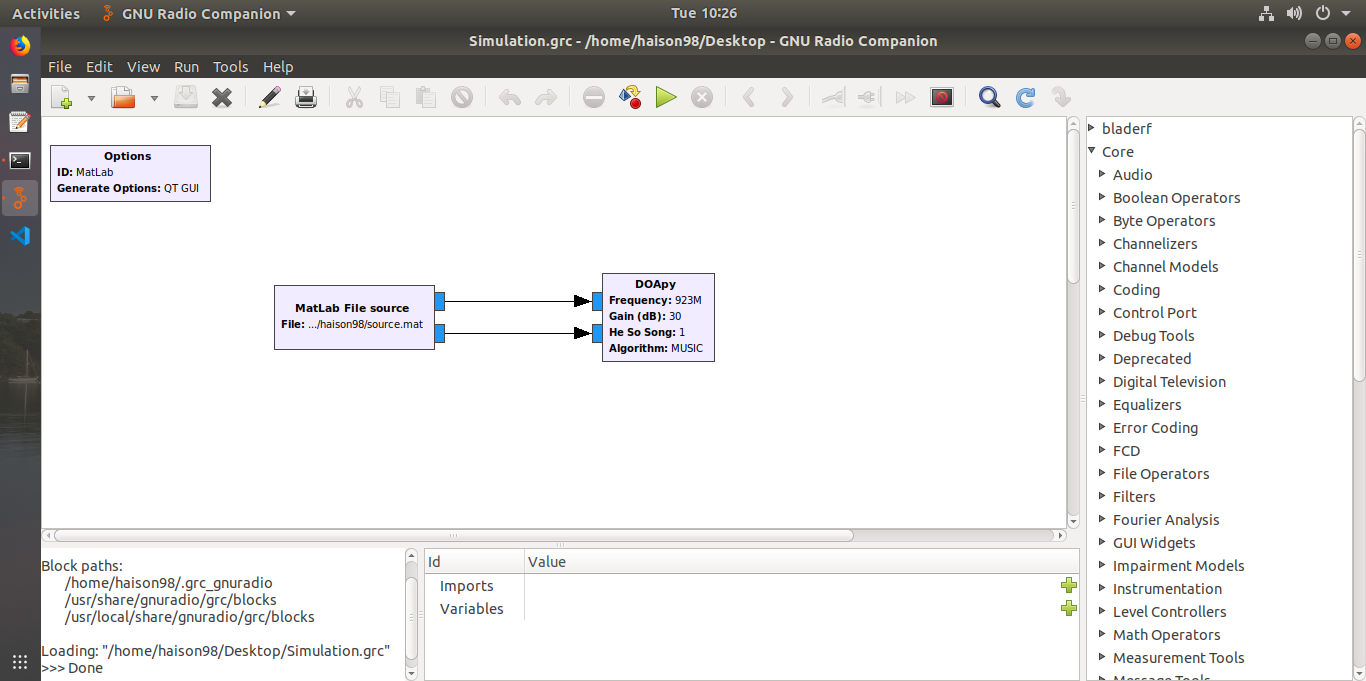
\includegraphics[width=1\linewidth]{figures/simulation1.png}
			\caption{Flow-graph ước lượng DOA với dữ liệu mô phỏng Matlab trên GNU Radio}
			\label{fig:simulation1}
			\end{figure} 
			\newpage}
	\item {
		Mô phỏng dữ liệu thu từ BladeRF, vừa chịu ảnh hưởng từ kênh truyền, vừa chịu ảnh hưởng do sai số phần cứng BladeRF gây ra.
		\renewcommand{\thefigure}{B.\arabic{figure}} 
		\setcounter{figure}{0}
		 \begin{figure}[!ht]
			%\hfill
			\centering
			\subfigure[Mô phỏng tạp âm và nhiễu đa đường]{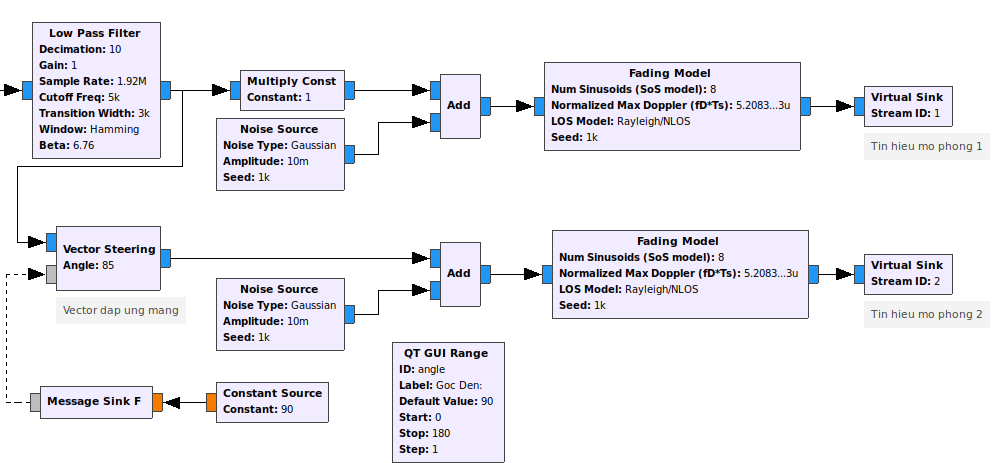
\includegraphics[width=1\linewidth]{figures/channel.png}
				\label{fig:channel}}
			\hfill
			\subfigure[Mô phỏng $\textrm{sample}_\textrm{offset}$ và $\textrm{phase}_\textrm{offset}$]{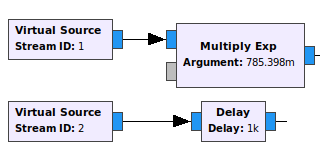
\includegraphics[width=0.5\linewidth]{figures/sampleandphase.png}\label{fig:sampleandphase}}
			\hfill
			\caption{Mô phỏng dữ liệu BladeRF qua kênh truyền}
			\label{fig:bladesimu}
		\end{figure}
	\newpage
	}

	\item {
		Flow-graph điều chế tín hiệu NBFM:
		\renewcommand{\thefigure}{C.\arabic{figure}} 
		\setcounter{figure}{0}
\begin{figure} [!h]
	\centering
	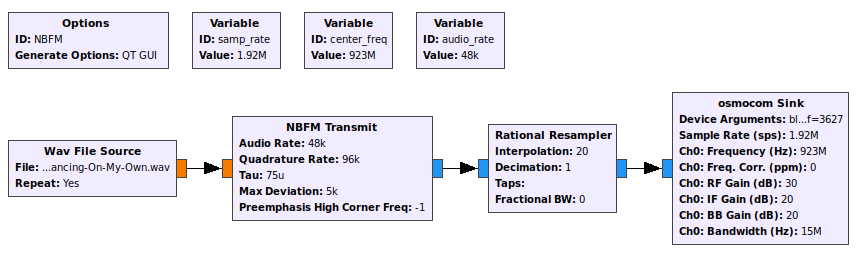
\includegraphics[width=1\linewidth]{figures/NBFM.png}
	\caption{Flow-graph truyền tín hiệu NBFM}
	\label{fig:NBFM}
\end{figure}
	\newpage	
}
	
	\item {
		Flow-graph của hệ DOA trên BladeRF, các khối tương ứng với chức năng chính:
		%\renewcommand{\labelitemi}{$-$}
		\begin{itemize}
			\item Osmosdr Source: khối nguồn lấy dữ liệu trực tiếp từ các SDR, được phát triển dưới dạng mã nguồn mở,  hỗ trợ rất nhiều loại SDR: RTL-SDR, USRP, BladeRF, HackRF, LimeSDR, ... Có sẵn hầu hết các thông số đầu vào như tần số thu, tốc độ lấy mẫu, băng thông, khuếch đại,... tất cả đều trực quan và dễ dàng chỉnh sửa. %APIs
			\item DC Blocker: loại bỏ thành phần một chiều trong tín hiệu.
			\item Low Pass Filter: bộ lọc thông thấp, dễ dàng chuyển đổi $f_\textrm{cut}$ tương ứng với trạng thái đồng bộ hoặc ước lượng DOA của hệ thống.
			\item Virtual Sink/Source: các khối chuyển tiếp dữ liệu, giúp thu gọn và chia luồng dữ liệu để tiện xử lý.
			\item $\textrm{Sample}_\textrm{offset}$: ước lượng mẫu offset do trễ đầu vào.
			\item PCA Phase Diff: tính toán độ lệch pha giữa 2 tín hiệu cho bước đồng bộ SDR.
			\item Probe Signal/Funcion Probe: lưu giá trị đầu vào dưới dạng biến làm thông số cho các khối khác.
			\item DOA/DOA Python: khối ước lượng DOA được viết trên ngôn ngữ tương ứng C++/Python.
			\item QT GUI: các khối hiển thị giao diện người dùng.
		\end{itemize}
		
		
		\renewcommand{\thefigure}{D.\arabic{figure}} 
		\setcounter{figure}{0}
		\afterpage{\clearpage}
		\begin{figure} [!ht]
			\centering
			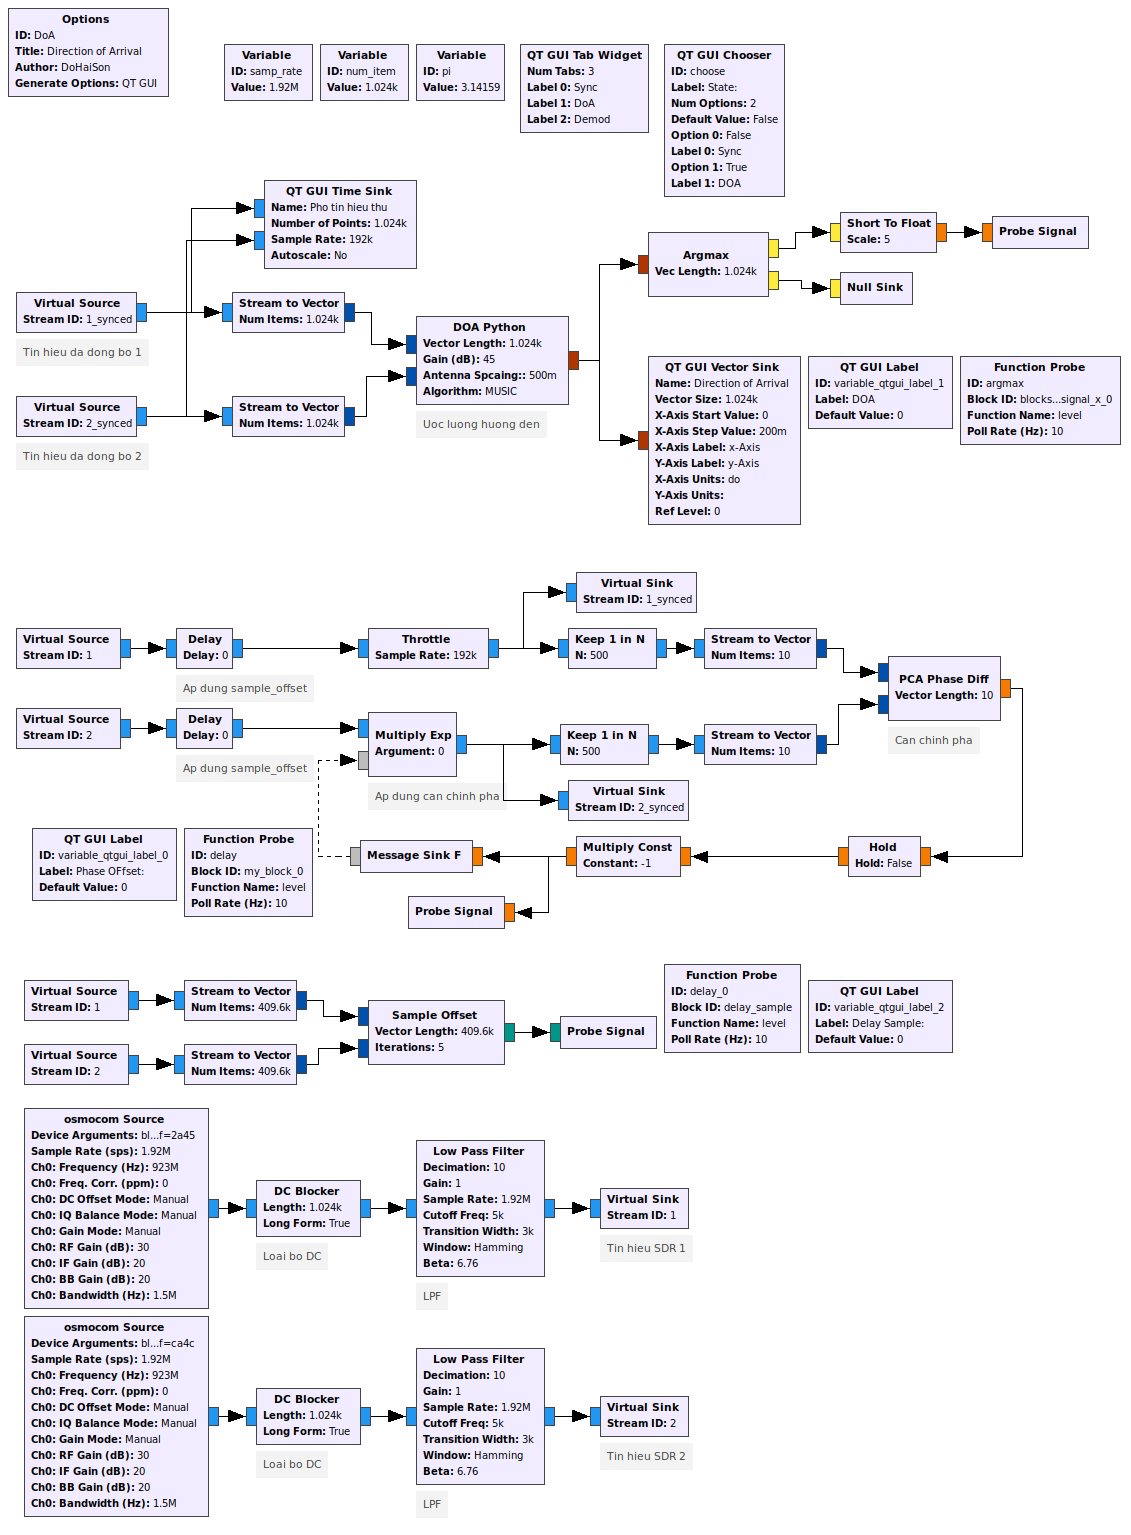
\includegraphics[width=\textwidth,height=\textheight,keepaspectratio]{figures/DoA_FM_grc.png}
			\caption{Flow-graph ước lượng DOA}
			\label{fig:DoA_FM}
		\end{figure}
	\newpage
	}
	
	\item {
		Flow-graph điều chế tín hiệu truyền hình chuẩn DVB-T trên GNU Radio.
	\renewcommand{\thefigure}{E.\arabic{figure}} 
	\setcounter{figure}{0}
	\begin{figure} [!h]
		\centering
		\includegraphics[width=0.95\linewidth]{figures/dvbt.png}
		\caption{Flow-graph truyền tín hiệu DVB-T}
		\label{fig:dvbt}
	\end{figure}	
}
\end{enumerate}
\def\baselinestretch{1}
\vspace{-2cm}
\renewcommand{\bibname}{Tài liệu tham khảo}
\clearpage
\phantomsection
\addcontentsline{toc}{chapter}{{TÀI LIỆU THAM KHẢO}}
\renewcommand{\refname}{Literary works}
\begin{thebibliography}{xx}
	\section*{Tiếng Việt}
	\vspace{0.3cm}
	\harvarditem{Quỳnh}{2015}{Quynh2015}
	Trần Thị Thúy Quỳnh , {\em {Nghi{\^{e}}n cứu
			n{\^{a}}ng cao hiệu năng của hệ t{\`{i}}m phương sử dụng anten
			kh{\^{o}}ng tầm pha trong m{\^{o}}i trường c{\'{a}}c nguồn t{\'{i}}n
			hiệu tương quan}}, Luận án tiến sĩ, 2015, tr.~19--23.
	\vspace{0.5cm}	
	\section*{Tiếng Anh}	
	
	\harvarditem{Feickert}{2005}{Feickert2005}
	Andrew Feickert, ``{The Joint Tactical
		Radio System (JTRS) and the Army{\'{s}} Future Combat System (FCS): Issues
		for Congress}'', {\em Congressional Research Service: Report}, 2005, pp.~1.
	
	\harvarditem[Bloessl et~al.]{Bloessl, Segata, Sommer \harvardand\
		Dressler}{2013}{Bloessl2013}
	B. Bloessl, M. Segata, C. Sommer \harvardand\ F. Dressler, ``An IEEE802.11a/g/p OFDM receiver for GNU radio'',
	{\em SRIF 2013 - Proceedings of the 2nd, 2013 ACM SIGCOMM Workshop on
	Software Radio Implementation Forum}, 2013, pp.~9--15.

	\harvarditem{BogdanDIA}{2015}{BogdanDIA2015}
	BogdanDIA  , ``{DVB-T implementation in gnuradio}'', 2015.
	\newline{[Online]. Available: $https://github.com/BogdanDIA/gr-dvbt$}

	\harvarditem[Bergstrom et~al.]{Bergstrom, Chuprun, Gifford \harvardand\
	Maalouli}{2002}{Bergstrom2002}
	C. Bergstrom, S. Chuprun, S. Gifford, \harvardand\ G. Maalouli
	, ``{Software defined radio (SDR)
	special military applications}'', {\em MILCOM 2002. Proceedings},
	{vol.~1}, 2002, pp.~383--388.
	
	\harvarditem{Bellini \harvardand\ Tosi}{1907}{Bellini1907}
	E. Bellini \harvardand\ A. Tosi,
	``{A directive system of wireless telegraphy}'', {\em Proceedings of the
		Physical Society of London}, vol.~21, no.~1, 1907, pp.~305--328.
	
	\harvarditem[Gomez-Miguelez et~al.]{Gomez-Miguelez, Garcia-Saavedra, Sutton,
		Serrano, Cano \harvardand\ Leith}{2016}{Gomez-Miguelez2016}
	I. Gomez-Miguelez, A. Garcia-Saavedra, Paul D. Sutton, P. Serrano, C. Cano
	\harvardand\ Douglas J. Leith,
	``{srsLTE: An open-source platform for LTE evolution and experimentation}'',
	{\em Proceedings of the Annual International Conference on Mobile Computing
		and Networking, MOBICOM}, 2016, pp.~25--32.
	
	\harvarditem{Ziskind \harvardand\ Wax}{1988}{Ziskind1988}
	I. Ziskind \harvardand\ M. Wax,
	``{Maximum Likelihood Localization of Multiple Sources by Alternating
		Projection}'', {\em IEEE Transactions on Acoustics, Speech, and Signal
		Processing}, {vol.~36}, no.~10, 1988, pp.~1553--1560.
	
	\harvarditem{Capon}{1969}{Capon2009}
	J. Capon, ``{High-resolution frequency-wavenumber spectrum analysis}'', 
	{\em Proceedings of the IEEE}, {vol.~57}, no.~8, 1969, pp.~1408--1418.
	
	\harvarditem{Liberti \harvardand\ Rappaport}{1999}{Liberti1999}
	Joseph C. Liberti \harvardand\ Theodore S. Rappaport, {\em Smart antennas for wireless communications: IS-95 and third generation CDMA applications}, 
	{Prentice Hall PTR}, 1999, pp.~134--134.
	
	\harvarditem{{Van Rijsbergen}}{n.d.}{VanRijsbergen}
	Kenneth van Rijsbergen, ``{The
		effectiveness of a homemade IMSI catcher build with YateBTS and a BladeRF}'', {\em Semanticscholar}, 2016.
	
	\harvarditem{{\em {KerberosSDR Demo software for direction finding and passive
				radar}}}{2019}{kerberos}
	{KerberosSDR: ``Demo software for direction finding and passive radar''}, 2019.
	\newline{[Online]. Available: $https://github.com/rtlsdrblog/kerberossdr$}
	
	\harvarditem{Nentwig}{2016}{Nentwig2016}
	M. Nentwig, ``{Delay estimation by FFT}'', {\em DSPRelated}, 2016.
	
	\harvarditem{{\em {DC offset and IQ Imbalance Correction {\textperiodcentered}
				Nuand/bladeRF Wiki}}}{n.d.}{Dccali}
	{ {Nuand/bladeRF, ``DC offset and IQ Imbalance Correction''.}} 
	\newline{[Online]. Available: $https://github.com/Nuand/bladeRF/wiki/DC-offset-and-IQ-Imbalance-Correction$}
	
	\harvarditem{{\em {Nuand: kalibrate-bladeRF}}}{2010}{kali}
	{Nuand/bladeRF: ``kalibrate-bladeRF''}, 2010.
	\newline{[Online]. Available: $https://github.com/Nuand/kalibrate-bladeRF$}
	
	\harvarditem[Kavitha et~al.]{Kavitha, {Meera Mohan}, Surya, Gandhiraj
		\harvardand\ Soman}{2015}{Kavitha2015}
	P. Kavitha, K. Meera Mohan, R. Surya, R. Gandhiraj \harvardand\ K.P. Soman, {``Implementation of CDMA in GNU radio''}, {\em Procedia Computer Science}, vol.~46, 2015, pp.~981--988.
	
	\harvarditem{Krysik}{2016}{multi-rtl}
	P. Krysik, ``{Multi-channel receiver with use of RTL-SDR dongles}'', 2016.
	\newline{[Online]. Available: $https://github.com/ptrkrysik/multi-rtl$}
	
	\harvarditem{Nehorai \harvardand\ A.}{1989}{Transactions1989}
	P. Stoica \harvardand\ A. Nehorai,
	``{MUSIC, Maximum Likelihood, and Cramer-Rao Bound}'', {\em IEEE Transactions
		on Acoustics, Speech, and Signal Processing}, {vol.~37}, no.~5, 1989.
	
	\harvarditem{{\em {PyBOMBS (Python Build Overlay Managed Bundle
				System)}}}{n.d.}{PyBombs}
	PyBOMBS: ``Python Build Overlay Managed Bundle System''.
	\newline{[Online]. Available: $https://github.com/gnuradio/pybombs$}
	
	\harvarditem{Bracewell}{1978}{Bracewell1978}
	Ronald N. Bracewell, {\em {The Fourier Transform and Its Applications}}, McGraw-Hill, 1978, pp.~46 and 243.
	
	\harvarditem{{R. I. Lackey and D. W. Upmal}}{1995}{Fakhrian2012}
	{R. I. Lackey and D. W. Upmal},
	``{Speakeasy: The Military Software Radio}'', {\em IEEE Communications
		Magazine}, {vol.~33}, no.~5, 1995, pp.~56--61.
	
	\harvarditem{Keen}{1922}{Darwin1895}
	R. Keen, {\em {Direction and Position Finding by Wireless}}, 1922.
	
	\harvarditem{Schmidt}{1986}{Schmidt2009a}
	R. Schmidt, ``{Multiple emitter
		location and signal parameter estimation}'', {\em IEEE Transactions on Antennas and Propagation}, vol.~34, no.~3, 1986, pp~276--280.
	
	\harvarditem[Whiting et~al.]{Whiting, Sorensen, Moon \harvardand\
		Gunther}{2018}{Whiting2018}
	S. Whiting, D. Sorensen, T. K. Moon \harvardand\ J. H. Gunther,
	 ``{Time and frequency corrections in
		a distributed radio network}'', {\em 2017 51st Asilomar Conference on Signals, Systems, and Computers}, 2017, pp.~1123--1126.
	
	\harvarditem{{Travis F Collins}}{n.d.}{TravisFCollins}
	 Srikanth Pagadarai, Travis Collins and Alexander M. Wyglinski, ``{Phase
		Synchronization Capability of TwinRX Daughterboards and DoA Estimation}'', {\em Ettus Research}, 2016, pp.~1--12.
	
\end{thebibliography}

\end{document}
